% Ερευνητική πρόταση διδακτορικής διατριβής, v8.78 (από v8.75) — σύντομη αυτοτελής πρόταση, συγχρονισμένη με την εκτενή v8.71g.
% Εκτενής πρόταση: v8.71g. Αναλυτικό τεχνικό πρωτόκολλο: v8.71g. Συνοδευτικά: Μουσικολογικό παράρτημα και επεκτάσεις.
% Μεταγλώττιση: XeLaTeX, δύο περάσματα.
\documentclass[11pt,a4paper]{article}
\usepackage[a4paper,left=1.65cm,right=1.65cm,top=1.44cm,bottom=1.45cm,headheight=14pt,headsep=6.5mm]{geometry}
\usepackage{fontspec,polyglossia}
\setdefaultlanguage{greek}
\setotherlanguage{english}
\setmainfont{FreeSerif}[Ligatures=TeX]
\newfontfamily\greekfont{FreeSerif}[Ligatures=TeX]
\newfontfamily\englishfont{FreeSerif}[Ligatures=TeX]
\setsansfont{FreeSans}[Scale=MatchLowercase]
\newfontfamily\greekfontsf{FreeSans}[Scale=MatchLowercase]
\setmonofont{DejaVu Sans Mono}[Scale=MatchLowercase]
\newfontfamily\greekfonttt{DejaVu Sans Mono}[Scale=MatchLowercase]
\usepackage{microtype,amsmath,amssymb,graphicx,tabularx,booktabs,array,ragged2e,longtable,calc}
\usepackage{xcolor,hyperref,fancyhdr,titlesec,enumitem,needspace}
\usepackage{tikz}
\usepackage{float}
\usetikzlibrary{positioning,arrows.meta,shapes.geometric,calc,fit}
\usepackage{indentfirst}
\definecolor{acc}{HTML}{7A2E2E}
\definecolor{soft}{HTML}{F7F1F1}
\definecolor{edge}{HTML}{8A8A8A}
\hypersetup{colorlinks=true,linkcolor=acc,citecolor=acc,urlcolor=acc,
 pdftitle={Ερευνητική πρόταση: Η μουσική θέση ως υπολογιστική μονάδα της βυζαντινής μουσικής},
 pdfauthor={Γεώργιος Σπυριδάκης},pdfsubject={Συμβολική αναπαράσταση, ιστορική μετάδοση και γνωσιακή λειτουργία}}
\newcolumntype{Y}{>{\raggedright\arraybackslash}X}
\newcolumntype{L}[1]{>{\raggedright\arraybackslash}p{#1}}
\setlength{\parindent}{1em}
\setlength{\parskip}{1.75pt}
\setlength{\tabcolsep}{3.5pt}
\renewcommand{\arraystretch}{1.09}
\emergencystretch=2em
\raggedbottom
\widowpenalty=10000
\clubpenalty=10000
\titleformat{\section}{\large\bfseries\color{acc}}{\thesection.}{0.5em}{}
\titleformat{\subsection}{\normalsize\bfseries\color{acc}}{\thesubsection}{0.5em}{}
\titlespacing*{\section}{0pt}{8pt}{4pt}
\titlespacing*{\subsection}{0pt}{5.5pt}{3pt}
\pagestyle{fancy}
\fancyhf{}
\lhead{\footnotesize Γ. Σπυριδάκης / Ερευνητική πρόταση}
\rhead{\footnotesize\thepage}
\renewcommand{\headrulewidth}{0.3pt}
\newcommand{\keybox}[1]{\par\smallskip\noindent\fcolorbox{acc}{soft}{\parbox{\dimexpr\linewidth-2\fboxsep-2\fboxrule\relax}{\setlength{\parindent}{0pt}#1}}\par\smallskip}
\newcommand{\fullspec}[1]{\par\noindent{\footnotesize\color{black!65} Αναλυτική προδιαγραφή στην εκτενή πρόταση v8.71g: #1.}\par}
\newcommand{\figcap}[2]{\par\vspace{3pt}\begin{minipage}{0.95\linewidth}\footnotesize\textbf{#1} #2\end{minipage}\par}
\newcommand{\dhist}{\Delta_{\mathrm{hist}}}
\newcommand{\Mth}{M\textsubscript{θέσις}}
\newenvironment{reflist}{\begin{list}{}{\leftmargin=1.4em\itemindent=-1.4em\itemsep=0.8pt\parsep=0pt}\small}{\end{list}}
\setlist[itemize]{leftmargin=1.4em,itemsep=1pt,topsep=2pt}
\setlist[enumerate]{leftmargin=1.6em,itemsep=1pt,topsep=2pt}
\graphicspath{{assets/}}
\tikzset{
 box/.style={draw=edge,rounded corners=3pt,line width=0.6pt,align=center,font=\footnotesize,inner sep=3pt},
 mainbox/.style={box,draw=acc,line width=1.1pt,fill=soft},
 gatebox/.style={box,dashed},
 arr/.style={-{Stealth[length=2.2mm]},draw=edge,line width=0.6pt},
 lane/.style={font=\footnotesize\itshape,text=black!60,anchor=west}
}
\begin{document}
\fontsize{10.32}{11.91}\selectfont
\raggedright
\setlength{\parindent}{1em}

% ------------------------------------------------------------------
\begin{titlepage}
\centering
\vspace*{0.7cm}
{\sffamily\large ΕΛΛΗΝΙΚΟ ΜΕΣΟΓΕΙΑΚΟ ΠΑΝΕΠΙΣΤΗΜΙΟ\par}
{\sffamily Τμήμα Μουσικής Τεχνολογίας και Ακουστικής\par}
\vspace{1.6cm}
{\Large\bfseries\color{acc} ΕΡΕΥΝΗΤΙΚΗ ΠΡΟΤΑΣΗ\par}
\vspace{1.2cm}
{\fontsize{22}{27}\selectfont\bfseries Η μουσική θέση ως υπολογιστική μονάδα της βυζαντινής μουσικής\par}
\vspace{0.6cm}
{\Large Συμβολική αναπαράσταση, ιστορική μετάδοση και γνωσιακή λειτουργία\par}
\vspace{0.5cm}
{\large\itshape The Byzantine melodic formula as a computational unit in New Method chant\par}
\vspace{1.1cm}

\vfill
\begin{tabularx}{0.94\linewidth}{@{}>{\bfseries}L{3.9cm}Y@{}}
Υποψήφιος & Γεώργιος Σπυριδάκης\\[8pt]
Γνωστικό πεδίο & Συμβολική Ανάκτηση Μουσικής Πληροφορίας, μηχανική μάθηση αναπαραστάσεων, υπολογιστική μουσικολογία και μουσική γνωσιακή επιστήμη\\[8pt]
Μουσικό πεδίο & Μουσικές θέσεις σε Χερουβικά και Κοινωνικά της Νέας Μεθόδου\\[8pt]
Χρονικός ορίζοντας & 48 μήνες\\[8pt]
Συνοδευτικά κείμενα & Εκτενής τεχνική πρόταση και μουσικολογικό παράρτημα (διαθέσιμα κατόπιν αιτήματος)\\[8pt]
Ημερομηνία & Οκτώβριος 2026
\end{tabularx}
\vspace{0.3cm}
\end{titlepage}
\setcounter{page}{1}

% ------------------------------------------------------------------
\section*{Περίληψη}
Στη βυζαντινή ψαλτική της Νέας Μεθόδου, η μουσική θέση αποτελεί ιστορικά αναγνωρίσιμο μελικό σχηματισμό μεταβλητής έκτασης. Η ίδια θέση μπορεί να εμφανίζεται με αισθητά διαφορετική μελωδική ανάπτυξη, ενώ επιφανειακά συγγενή χωρία μπορούν να ανήκουν σε διαφορετικές θέσεις. Η παράδοση διασώζει επίσης ένα ιδιαίτερα σημαντικό ιστορικό τεκμήριο: τις εξηγήσεις, με τις οποίες παλαιότερα μέλη αποδόθηκαν στην αναλυτική γραφή της Νέας Μεθόδου. Σε ορισμένες περιπτώσεις διατίθενται παράλληλες εξηγήσεις του ίδιου χωρίου, ιδίως από τον Γρηγόριο Πρωτοψάλτη και τον Χουρμούζιο Χαρτοφύλακα.

Η έρευνα οργανώνεται σε δύο συνδεδεμένες υπολογιστικές διαδρομές. Η πρώτη εξετάζει τη μουσική θέση ως μονάδα συμβολικού Music Information Retrieval: αναπτύσσει μεθόδους κοινής οριοθέτησης και αναγνώρισης οικογενειών μέσα στη συνεχή ροή, με αμφίσημα όρια και δυνατότητα αιτιολογημένης αποχής. Ελέγχει επίσης αν οι ιστορικά τεκμηριωμένες εξηγητικές σχέσεις παρέχουν πρόσθετη πληροφορία για τη μάθηση μουσικών αναπαραστάσεων σε σύγκριση με ζεύγη κοινής οικογένειας. Η κύρια αντίθεση αξιολογείται μέσω ανεξάρτητων εκτελεστικών μετρήσεων, με κοινό μοντέλο και αντιστοιχισμένες συνθήκες εκπαίδευσης.

Η δεύτερη διαδρομή εξετάζει πόση πληροφορία της παλαιότερης σημειογραφίας παραμένει ανακτήσιμη από την εξήγηση. Διαφορετικά ιστορικά σημάδια μπορούν να έχουν κοινή μετροφωνική ανάγνωση, αφήνοντας ανοιχτό το ερώτημα αν η αναλυτική απόδοση περιέχει στοιχεία που διακρίνουν τη συγκεκριμένη γραφική επιλογή. Ένα πιθανοτικό μοντέλο μετρά τη βελτίωση της ανάκτησης όταν προστίθεται μία εξήγηση και, όπου σώζεται, μία δεύτερη· η ιστορική ανάγνωση του μάρτυρα παρέχει το ανεξάρτητο κριτήριο. Σε επόμενο στάδιο εξετάζεται αν οι αναπαραστάσεις που μαθαίνουν οικογενειακή ταυτότητα διατηρούν προσβάσιμες αυτές τις ιστορικές διακρίσεις.

Τα αποτελέσματα εξετάζονται με τυφλές κρίσεις ειδικών, δοκιμασίες μουσικής προσδοκίας και αντιληπτικής οργάνωσης κατά οικογένεια, μετρήσεις σύγχρονης εκτέλεσης και εφαρμογή σε πλήρη έργα του Νικολάου Πρωτοψάλτη Σμύρνης. Το ερευνητικό πρόγραμμα προβλέπει επίσης στοχευμένες πιλοτικές μελέτες μουσικολογικής διαγνωστικότητας και πιθανοτικής πραγμάτωσης, ανάλογα με την επάρκεια των δεδομένων. Κύρια παραδοτέα είναι ένα τεκμηριωμένο σώμα αξιολόγησης σε επίπεδο θέσης, μια ελεγχόμενη εκτίμηση της αξίας της ιστορικής εποπτείας, ένας εμπειρικός χάρτης ανακτησιμότητας της παλαιότερης γραφής και ένα ερμηνεύσιμο πλαίσιο μουσικολογικής ανάλυσης.

\noindent\textbf{Λέξεις-κλειδιά:} βυζαντινή ψαλτική, Νέα Μέθοδος, μουσική θέση, εξήγηση, συμβολικό MIR, μάθηση αναπαραστάσεων, αντίστροφη ανάκτηση, μουσικολογικά ενημερωμένη μηχανική μάθηση.

\begin{otherlanguage}{english}
\section*{Abstract}
In New Method Byzantine chant, the melodic formula (\textgreek{θέση}) is a historically recognised unit of variable length. A formula may recur with substantially different melodic realisations, whereas superficially similar passages can belong to different formulae. The tradition also preserves a distinctive historical record: the exegeses through which older repertory was rendered in the analytical New Method notation. Some passages survive in parallel exegeses, including those attributed to Gregorios the Protopsaltes and Chourmouzios the Chartophylax.

This doctoral project follows two connected computational routes. The first develops symbolic music information retrieval methods for joint segmentation and family recognition in continuous chant, accommodating uncertain boundaries and principled abstention. It tests whether historically documented same-passage exegesis relations contribute additional information to representation learning beyond shared-family supervision. The main comparison uses matched training conditions and an independent criterion derived from present-day performance variation.

The second route investigates which distinctions in older written notation remain recoverable from analytical exegeses. Different historical signs can share the same metrophonic reading; probabilistic inverse modelling therefore tests whether a first exegesis, and where available a second exegesis, improves prediction of the sign recorded by an independently examined historical witness. A subsequent evaluation asks whether family-oriented neural representations retain access to these distinctions.

Independent expert judgements, behavioural listening experiments on melodic expectation and categorisation, acoustic performance measurements, and comparative analyses of complete works by Nikolaos Protopsaltes of Smyrna provide complementary validation. Additional pilots study the role of diagnostic musicological knowledge and the predictability of melodic realisation, subject to independently established data-sufficiency criteria. The anticipated contributions include a provenance-auditable formula-level benchmark, a controlled assessment of historically informed supervision, an empirical map of older-notation recoverability, and an interpretable framework for Byzantine musical analysis.

\noindent\textbf{Keywords:} Byzantine chant, New Method notation, melodic formula, exegesis, symbolic MIR, representation learning, inverse recovery, musicology-informed machine learning.
\end{otherlanguage}

% ------------------------------------------------------------------
\section{Εισαγωγή: πρόβλημα και κίνητρο}

\subsection{Το πρόβλημα MIR και η μουσική θέση}
Η υπολογιστική μελέτη ενός μουσικού έργου αρχίζει με μια επιλογή που καθορίζει ολόκληρη την ανάλυση: σε ποιες μονάδες θα αναπαρασταθεί η μουσική; Μια ακολουθία από μεμονωμένα σημειογραφικά ή μελωδικά γεγονότα επιτρέπει την περιγραφή τοπικών κινήσεων. Η αναγνώριση όμως επαναλαμβανόμενων μελικών σχηματισμών, οι οποίοι ενδέχεται να αλλάζουν σε έκταση και εσωτερική ανάπτυξη, προϋποθέτει τη μελέτη μεγαλύτερων μονάδων και των σχέσεων μεταξύ τους. Στο συμβολικό Music Information Retrieval (MIR, ανάκτηση μουσικής πληροφορίας από ψηφιακά κωδικοποιημένη μουσική γραφή), η επιλογή της μονάδας επηρεάζει επομένως τόσο την τμηματοποίηση όσο και τη μάθηση μουσικής ταυτότητας.

Η στατιστικά κατάλληλη τμηματοποίηση ενδέχεται να διαφοροποιείται από τη μονάδα που αναγνωρίζει μια συγκεκριμένη μουσική παράδοση (V.~Lanz και J.~Hajič~Jr., 2025). Έτσι προκύπτει ένα πρώτο ερώτημα: με ποια αναπαράσταση εντοπίζονται μουσικά σημαντικά τμήματα μεταβλητού μήκους; Ακολουθεί ένα δεύτερο: ποια τεκμήρια επιτρέπουν στο μοντέλο να αναγνωρίσει ότι δύο διαφορετικές πραγματώσεις μοιράζονται μια κοινή ταυτότητα; Στη σύγχρονη μάθηση αναπαραστάσεων τα θετικά ζεύγη προέρχονται συχνά από τεχνητούς μετασχηματισμούς ή από κοινές ετικέτες. Η βυζαντινή ψαλτική προσφέρει τη δυνατότητα να ελεγχθούν και τα δύο ερωτήματα μέσα σε παράδοση με ιστορικά αναγνωρίσιμες μελικές μονάδες και σωζόμενες σχέσεις μεταξύ διαφορετικών αποδόσεών τους.

Για να κατανοηθεί γιατί η ψαλτική αποτελεί κατάλληλο πεδίο ελέγχου, χρειάζεται να διακριθεί η μουσική γραφή από τη μουσική οργάνωση που περιγράφει. Η \textbf{Νέα Μέθοδος}, που καθιερώθηκε το 1814 με τη συμβολή του Χρυσάνθου εκ Μαδύτων, του Γρηγορίου Πρωτοψάλτη και του Χουρμουζίου Χαρτοφύλακα, χρησιμοποιεί \emph{νεύματα}: σημάδια που δηλώνουν σχετικές μελωδικές κινήσεις και συνδυάζονται με χρονικές και ποιοτικές ενδείξεις. Η σημασία τους εξαρτάται επίσης από τον \emph{ήχο}, δηλαδή την τροπική οργάνωση μέσα στο σύστημα της οκταηχίας. Μέσα από τις σχέσεις αυτών των σημαδιών περιγράφονται ατομικά μελωδικά γεγονότα και συγκροτούνται μεγαλύτεροι μελικοί σχηματισμοί.

Σε αυτό το επίπεδο οργάνωσης εντάσσεται η \textbf{μουσική θέση}: μελικός σχηματισμός μεταβλητής έκτασης, ο οποίος μπορεί να αναγνωρίζεται σε διαφορετικά έργα και πηγές μέσα από κοινές δομικές μουσικές σχέσεις. Η συγκεκριμένη μορφή του επηρεάζεται από τη βαθμίδα, τον ήχο, τη συλλαβική κατανομή του κειμένου και την αναλυτικότητα της γραφής. Η \emph{πραγμάτωση} δηλώνει αυτή τη συγκεκριμένη μορφή, ενώ η \emph{οικογενειακή ταυτότητα} θα προσδιοριστεί με μουσικολογικά τεκμηριωμένα διαγνωστικά κριτήρια. Η διάκριση ανάμεσα στα δύο επιτρέπει να εξεταστεί μετρήσιμα η ταυτότητα μέσα στη μεταβολή.

Η ανάγκη αυτής της διάκρισης φαίνεται στις ιστορικές συγκρίσεις. Η \emph{μετροφωνία} περιγράφει την ανάγνωση των σημειογραφικών ποσοτικών κινήσεων και διακρίνεται αναλυτικά από την πληρέστερη μελική πραγμάτωση. Το υπολογιστικό πρόβλημα έχει δύο όψεις, που τεκμηριώνονται στη διατριβή του Κ.~Χ.~Καραγκούνη (2003) για το μέλος των Χερουβικών. Συγγενής μετροφωνική επιφάνεια μπορεί να αντιστοιχεί σε διαφορετικές ιστορικές θέσεις (σ.~788). Αντίστροφα, θέσεις με ιδιαίτερα τροπικά συμφραζόμενα πραγματώνονται αισθητά διαφορετικά (σσ.~810--812). Ο Ι.~Αρβανίτης (2010, τ.~Α΄, §5.2, σσ.~136--142) δείχνει επίσης ότι μια θέση παραμένει αναγνωρίσιμη παρά τις διαφορές συλλαβικής κατανομής και τονισμού.

Από αυτές τις περιπτώσεις προκύπτουν δύο διαφορετικές υπολογιστικές δυσκολίες: συγγενείς επιφανειακές ακολουθίες μπορεί να οδηγήσουν σε εσφαλμένη ταύτιση, ενώ εκτεταμένες παραλλαγές μπορεί να αποκρύψουν κοινή μουσική ταυτότητα. Η έρευνα εξετάζει έτσι την από κοινού εκτίμηση ορίων και οικογενειακής ένταξης σε μονάδες μεταβλητού μήκους, διατηρώντας τις τεκμηριωμένες εναλλακτικές αναλύσεις όπου απαιτείται.

Η διάκριση ανάμεσα στα επίπεδα γίνεται σαφέστερη όταν ακολουθήσουμε τη μουσική οργάνωση από τα νεύματα έως το πλήρες έργο. Η θέση αποτελεί τον ενδιάμεσο μορφολογικό βαθμό που συνδέει την τοπική μουσική πληροφορία με την οργάνωση φράσεων και ευρύτερων μελών. Στο Σχήμα~1 η οικογένεια εμφανίζεται ως σχέση ταυτότητας μεταξύ πραγματώσεων, καθώς η οικογενειακή ταξινόμηση αφορά τη σύγκριση εμφανίσεων και όχι ένα επιπλέον στάδιο χρονικής σύνθεσης.

\begin{center}
\begin{tikzpicture}[
    font=\footnotesize,
    lev/.style={draw=black!42,rounded corners=3pt,fill=black!3,align=center,
       text width=2.65cm,minimum height=1.65cm,inner sep=3.5pt},
    central/.style={lev,draw=acc,line width=1.25pt,fill=soft,
       text width=2.70cm},
    link/.style={-{Stealth[length=2mm]},draw=black!55,line width=0.7pt},
    relation/.style={-{Stealth[length=2mm]},draw=acc,dashed,line width=0.7pt}
]
\node[lev] (neume) {\textbf{Νεύματα}\\\scriptsize Σημειογραφικές ενδείξεις};
\node[lev,right=0.48cm of neume] (event) {\textbf{Μουσικά γεγονότα}\\\scriptsize και μονάδες εισόδου};
\node[central,right=0.48cm of event] (pos) {\textbf{Μουσική θέση}\\\scriptsize Ταυτότητα και μεταβλητή πραγμάτωση};
\node[lev,right=0.48cm of pos] (sequence) {\textbf{Ακολουθίες θέσεων}\\\scriptsize Φράσεις και ενότητες};
\node[lev,right=0.48cm of sequence] (work) {\textbf{Πλήρες μέλος}\\\scriptsize Συνολική μελοποιητική οργάνωση};
\draw[link] (neume.east)--(event.west);
\draw[link] (event.east)--(pos.west);
\draw[link] (pos.east)--(sequence.west);
\draw[link] (sequence.east)--(work.west);
\node[draw=acc!75,rounded corners=2pt,fill=soft,align=center,
    text width=3.5cm,inner sep=3pt,below=0.65cm of pos] (fam)
    {\textbf{Οικογένεια θέσεων}\\\scriptsize Κατηγορική σχέση μεταξύ εμφανίσεων};
\draw[relation] (pos.south)--(fam.north);
\end{tikzpicture}
\par\vspace{3pt}
\begin{minipage}{0.98\linewidth}\footnotesize
\textbf{Σχήμα 1.} Από τη νευματική σημειογραφία στη δομή του πλήρους μέλους:
η μουσική θέση ως ενδιάμεση μορφολογική και υπολογιστική μονάδα.
Η οικογένεια θέσεων περιγράφει σχέσεις ταυτότητας μεταξύ εμφανίσεων
και πραγματώσεων. Τα βέλη δηλώνουν επίπεδα οργάνωσης· η ακριβής
τμηματοποίηση και οικογενειακή ένταξη αξιολογούνται στις M1–M3.
\end{minipage}
\end{center}

\noindent\textbf{Γιατί η θέση και γιατί οικογένειες.} Η θέση επιλέγεται ως μονάδα για δύο λόγους. Μουσικολογικά, είναι η μονάδα με την οποία οι ιστορικές πηγές και η νεότερη μορφολογική έρευνα περιγράφουν και συγκρίνουν το μέλος (§2.1). Υπολογιστικά, είναι το επίπεδο στο οποίο μπορεί να εφαρμοστεί σε όλο το σώμα η σύγκριση που η υπάρχουσα έρευνα κάνει χειροκίνητα σε επιλεγμένα χωρία. Ένα μεμονωμένο σημάδι είναι υποπροσδιορισμένο, επειδή η ενέργειά του μεταβάλλεται ανάλογα με το περιβάλλον (Χρύσανθος, 1832, §408)· ένα πλήρες μέλος επαναλαμβάνεται πολύ σπάνια για να μαθευτεί από παραδείγματα. Η θέση επανέρχεται από έργο σε έργο, αλλά όχι ως η ίδια ακολουθία φθόγγων, και γι' αυτό η αναγνώρισή της δεν ανάγεται σε ταίριασμα προτύπου. Η έρευνα εργάζεται επομένως με \textbf{οικογένειες θέσεων}: σύνολα εμφανίσεων που ικανοποιούν τις ίδιες ρητές διαγνωστικές σχέσεις, ενώ διαφέρουν σε έκταση και μελισματική ανάπτυξη. Η έννοια συγγενεύει με τις οικογένειες μελωδιών της προφορικής παράδοσης (A.~Volk και P.~van~Kranenburg, 2012) και με τη διάκριση πυρηνικών φθόγγων και επιφανειακών φορμουλών στα σχήματα του γαλάντ ύφους (G.~Rabinovitch και A.~Carter-Enyi, 2024). Είναι αναλυτική και τυπολογική κατηγορία, όχι γενεαλογική· αν λειτουργεί και ως κατηγορία της ακρόασης εξετάζεται εμπειρικά στη Μ3.


Η ιεραρχία εξηγεί τη διαδρομή των ερευνητικών μελετών: η M1 εξετάζει ποια κωδικοποίηση επιτρέπει την αναγνώριση των θέσεων, η M2 διερευνά τη διατήρηση της ταυτότητάς τους μέσα στην ιστορική παραλλαγή και η M5 αξιοποιεί τις ακολουθίες τους για την περιγραφή πλήρων έργων. Ένα συγκεκριμένο καταλογικό παράδειγμα δείχνει αμέσως πώς η ίδια υποψήφια μουσική δομή μπορεί να εμφανίζεται με περισσότερες μελωδικές μορφές.

\begin{center}
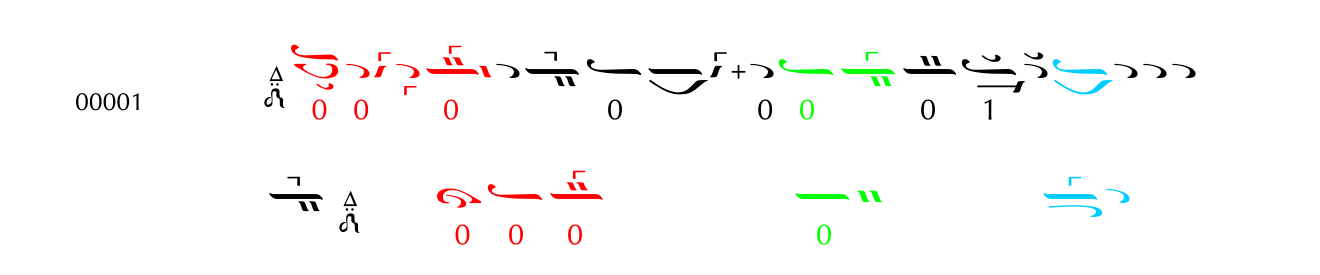
\includegraphics[width=0.88\linewidth]{formula_position_example.png}
\figcap{Σχήμα 2.}{Μελωδικός τύπος και καταγεγραμμένες παραλλαγές του σε κοινό προσωδιακό πρότυπο, από τη συλλογή \emph{Papadic Formulae} της Ιεράς Μονής Αγίου Αντωνίου. Η ακολουθία 00001 κωδικοποιεί πρότυπο πέντε συλλαβών (0: άτονη, 1: τονισμένη συλλαβή)· δεν είναι αναγνωριστικό θέσης. Οι έγχρωμες γραφές δηλώνουν παραλλαγές του ίδιου τύπου. Η τελική οικογενειακή απόδοση παραμένει αντικείμενο ανεξάρτητου ελέγχου.}
\end{center}

\subsection{Η εξήγηση ως ιστορικό τεκμήριο σχέσης}
Η μουσική θέση έχει ήδη παρουσιαστεί ως μονάδα που μπορεί να διατηρεί την ταυτότητά της μέσα σε διαφορετικές μορφές. Για να μάθει ένα υπολογιστικό σύστημα αυτή τη σχέση χρειάζεται παραδείγματα ταυτότητας και μεταβολής, των οποίων η προέλευση είναι γνωστή. Εδώ αποκτά ιδιαίτερη σημασία η ιστορία της ψαλτικής σημειογραφίας. Η παλαιότερη γραφή και η προφορική διδασκαλία μετέδιδαν μουσική γνώση με διαφορετικό βαθμό αναλυτικής καταγραφής. Η Νέα Μέθοδος επέτρεψε αναλυτικότερες σημειογραφικές αποδόσεις παλαιότερων μελών, διαδικασία που ονομάζεται \textbf{εξήγηση}.

Για αυτό το πρόβλημα η Νέα Μέθοδος διαθέτει ένα τεκμήριο ιδιαίτερης ερευνητικής αξίας: την ιστορικά επαληθεύσιμη σχέση ανάμεσα σε παράλληλες εξηγήσεις. Ο Γρηγόριος και ο Χουρμούζιος απέδωσαν σε αναλυτική γραφή πολλά από τα ίδια παλαιότερα μέλη. Οι παράλληλες εξηγήσεις του ίδιου χωρίου είναι ιστορικά τεκμηριωμένες πραγματώσεις του ίδιου μουσικού αντικειμένου. Η σχέση τους δεν προκύπτει από μελωδική ομοιότητα ούτε από την ταξινόμηση του ερευνητή· προκύπτει από τις πηγές.

Η τεκμηρίωση ότι δύο αναλυτικές αποδόσεις αντιστοιχούν στο ίδιο ιστορικό χωρίο προσφέρει μια σχέση μεταξύ συγκεκριμένων μουσικών πραγματώσεων. Η σχέση αυτή μπορεί να εισαχθεί στη μάθηση ως \emph{σχεσιακή εποπτεία}: το μοντέλο διδάσκεται ποιες εμφανίσεις σχετίζονται από τις πηγές και ελέγχεται αν αυτή η πληροφορία βελτιώνει την αναπαράσταση της ταυτότητας. Η ανεξάρτητη κρίση κοινής οικογένειας παραμένει πρόσθετη προϋπόθεση επιλογής των ζευγών. Η ερμηνεία αφορά τις σωζόμενες ιστορικές αποδόσεις· η ανακατασκευή της παλαιότερης εκτέλεσης εξετάζεται χωριστά στην ιστοριογραφία της εξήγησης (Γ.~Θ.~Στάθης, 1978· A.~Lingas, 2003· Αρβανίτης, 2022).

Η εξήγηση θέτει και ένα δεύτερο ερώτημα, αντίστροφο από εκείνο της αναγνώρισης της θέσης: πόση από τη γραπτή μορφή ενός παλαιότερου μουσικού χωρίου παραμένει αναγνωρίσιμη στην αναλυτική απόδοσή του; Στη νευματική γραφή διαφορετικά σημάδια μπορούν, υπό συγκεκριμένες συνθήκες, να έχουν την ίδια μετροφωνική ανάγνωση. Για παράδειγμα, το ολίγον και η πεταστή μπορούν να δηλώνουν την ίδια διαστηματική άνοδο, ενώ διαφοροποιούνται στη σημειογραφική και ποιοτική λειτουργία τους. Η περίπτωση χρησιμοποιείται εδώ ως θεωρητικό παράδειγμα· η ιστορική της αξιολόγηση θα στηριχθεί σε αυτοψία συγκεκριμένων μαρτύρων. Η ανάκτηση εξετάζει αν η εξήγηση επιτρέπει τη διάκριση τέτοιων παλαιότερων επιλογών, πέρα από τη μετροφωνία και το διαθέσιμο μουσικό περιβάλλον. Έτσι, η πρώτη διαδρομή μελετά την ταυτότητα της θέσης μέσα στη μεταβολή, ενώ η δεύτερη μετρά την ανακτησιμότητα μιας παλαιότερης σημειογραφικής διάκρισης από την ίδια μεταβολή. Οι δύο εργασίες συνδέονται μέσω των κοινών ιστορικών πηγών και συναντώνται στον μεταγενέστερο έλεγχο των μαθημένων αναπαραστάσεων. Συνδέονται και τεχνικά: ένα μοντέλο που περιγράφει πώς πραγματώνεται μια θέση στην αναλυτική γραφή μπορεί, αντεστραμμένο, να εκτιμήσει ποιες παλαιές γραφές είναι συμβατές με μια δεδομένη εξήγηση (§4.8).

\subsection{Βασικοί όροι}
Από τη θεωρητική θέση έως το ζεύγος εκπαίδευσης μεσολαβούν διαφορετικές έννοιες. Η \emph{οικογένεια} είναι κατηγορία κοινής διαγνωστικής μουσικής οργάνωσης· η \emph{πραγμάτωση} είναι μια συγκεκριμένη μουσική μορφή· η \emph{εμφάνιση} είναι ο εντοπισμός της σε ορισμένη πηγή. Η \emph{υπογραφή τύπου} δηλώνει τους κανόνες με τους οποίους κρίνεται η ένταξη. Ο πίνακας συνοψίζει τους ορισμούς που θα χρησιμοποιούνται σε όλη την έρευνα.

\begin{center}\small
\begin{tabularx}{\linewidth}{@{}>{\bfseries}L{3.1cm}Y@{}}
\toprule
Όρος & Ορισμός στην παρούσα έρευνα\\\midrule
Ιστορική θέση & Ο όρος ή η ονομασία ενός μελικού σχηματισμού στις πηγές. Είναι τεκμήριο, όχι έτοιμη ετικέτα κατηγορίας.\\
Οικογένεια θέσεων & Σύγχρονη αναλυτική και τυπολογική κατηγορία εμφανίσεων που ικανοποιούν τις ίδιες διαγνωστικές μουσικές σχέσεις σε δηλωμένη αναλυτική κλίμακα, παρά τις διαφορές έκτασης και επιφάνειας. Δεν είναι γενεαλογική κατηγορία· η γνωσιακή της υπόσταση ελέγχεται στη Μ3.\\
Υπογραφή τύπου & Ο ρητός κανόνας ένταξης μιας οικογένειας: διαγνωστικές σχέσεις, κανόνες περιβάλλοντος, κριτήρια αποκλεισμού. Επιτρέπει περισσότερες από μία επαρκείς διαμορφώσεις και οριστικοποιείται σε αριθμημένες εκδόσεις.\\
Πραγμάτωση & Η συγκεκριμένη μελωδική, χρονική, τροπική και σημειογραφική μορφή μιας θέσης σε έργο και πηγή.\\
Εμφάνιση & Εντοπισμένη παρουσία μιας πραγμάτωσης σε συγκεκριμένο χωρίο, με ένα ή περισσότερα αποδεκτά ζεύγη ορίων.\\
Εξηγητική σχέση & Τεκμηριωμένη σύνδεση μιας αναλυτικής απόδοσης με συγκεκριμένο παλαιότερο χωρίο. Δεν δημιουργεί από μόνη της οικογενειακή ένταξη.\\
Εκτέλεση & Η φωνητική και χρονική εκφορά μιας γραπτής πραγμάτωσης από ψάλτη. Διακρίνεται από τη σημειογραφική χρονική αξία.\\\bottomrule
\end{tabularx}
\end{center}

Οι διακρίσεις αυτές προστατεύουν την ερμηνεία της μηχανικής μάθησης: η υπολογιστική ομοιότητα, η οικογενειακή ένταξη και η ιστορικά τεκμηριωμένη εξήγηση παραμένουν χωριστά είδη σχέσεων.

\subsection{Η συνεισφορά της έρευνας}
Η κύρια συνεισφορά δεν είναι μια νέα αρχιτεκτονική. Βρίσκεται στη διατύπωση της υπολογιστικής εργασίας, στην πηγή της εποπτείας και στον τρόπο ελέγχου:
\keybox{\textbf{C1 — Νέα εργασία και σώμα αξιολόγησης.} Ταυτόχρονη οριοθέτηση και αναγνώριση θέσεων στη συνεχή ροή του μέλους, με εναλλακτικά όρια, ανοικτό σύνολο οικογενειών και αποχή· ανοικτό σώμα αξιολόγησης σε επίπεδο θέσης για τη Νέα Μέθοδο, το οποίο σήμερα δεν υπάρχει.\par\vspace{3pt}
\textbf{C2α — Ιστορική εποπτεία.} Ελεγχόμενη μέτρηση του τι προσθέτει η σχέση «ίδιο ιστορικό χωρίο» πέρα από τη σχέση «ίδια οικογένεια», με ανεξάρτητο κριτήριο από τη σύγχρονη εκτέλεση.\par\vspace{3pt}
\textbf{C2β — Η εξήγηση ως δρόμος προς την παλαιά γραφή.} Μέτρηση της πληροφορίας που διασώζει η εξήγηση για την παλαιά γραφή, πέρα από τη μετροφωνία και πέρα από τους γνωστούς κανόνες εξήγησης· εμπειρικός χάρτης ανακτησιμότητας.\par\vspace{3pt}
\textbf{C3 — Μουσικολογικά και γνωσιακά προϊόντα.} Ελέγξιμο λεξικό οικογενειών θέσεων, ποσοτική μορφολογία της εξήγησης, έλεγχος των θέσεων στην ακρόαση και την εκτέλεση, χαρακτηρισμός πλήρων έργων του Νικολάου Σμύρνης.}
Οι συνεισφορές, τα όριά τους και η αξία κάθε πιθανής έκβασης αναλύονται στην §8. Με αυτή τη βάση μπορούμε να εξετάσουμε τι γνωρίζει ήδη η μουσικολογία για τη θέση και ποιες συναφείς υπολογιστικές μέθοδοι έχουν αναπτυχθεί.

% ------------------------------------------------------------------
\section{Θεωρητικό πλαίσιο και βιβλιογραφική επισκόπηση}

\subsection{Η μουσικολογική γνώση για τη θέση και την εξήγηση}
Οι προηγούμενοι ορισμοί είναι λειτουργικοί για την παρούσα έρευνα και χρειάζονται ιστορική και βιβλιογραφική τεκμηρίωση. Η θέση έχει στέρεη ιστορική και μορφολογική θεμελίωση. Ο Μανουήλ Χρυσάφης, λαμπαδάριος και θεωρητικός του 15ου αιώνα, τη συνδέει με τη συνένωση σημείων που συγκροτεί μέλος (έκδ. D.~E.~Conomos, 1985b, σσ.~40--41). Ο Γαβριήλ ιερομόναχος χρησιμοποιεί τη γραμματική αναλογία της λέξης (έκδ. C.~Hannick και G.~Wolfram, 1985, σ.~72). Ο Χρύσανθος ο εκ Μαδύτων (1832, §§400, 408) περιγράφει τη μετάδοση και τις διαφορετικές ενέργειες των σημείων ανάλογα με το περιβάλλον τους.

Η ιστορική αυτή αναγνώριση μεγαλύτερων μουσικών σχηματισμών συνδέεται με τις νεότερες μελέτες της μορφολογίας τους. Από τη σύγχρονη έρευνα, ο Α.~Ε.~Αλυγιζάκης (1985, σσ.~81--82) περιγράφει τις θέσεις ως επαναχρησιμοποιούμενα μελικά πρότυπα που συγκροτούν φράσεις και ολοκληρωμένα μέλη. Ο Αρβανίτης (2010, §5.2) εξετάζει τη θέση ως αρχή μελικής ομοιότητας παρά τις διαφορές γραφής, τονισμού και συλλαβικής κατανομής. Ο C.~Troelsgård (2011), καθώς και η Μ.~Αλεξάνδρου με τον Troelsgård (2020, σσ.~175--180), εξηγούν τη σημειογραφική και τροπική λειτουργία αυτών των σχηματισμών.

Το ειδικό ρεπερτόριο της προτεινόμενης έρευνας είναι τα αργά μελισματικά Χερουβικά και Κοινωνικά, όπου μία συλλαβή μπορεί να αναπτύσσεται σε εκτενή μελωδική ακολουθία. Η έκταση αυτή προσφέρει πλούσιο υλικό για τη μελέτη της εσωτερικής δομής των θέσεων και επιτρέπει συγκρίσεις έργων με κοινό λειτουργικό κείμενο. Για το παπαδικό ρεπερτόριο, η μορφολογική και παλαιογραφική έρευνα έχει καταγράψει ονομασμένες θέσεις, επανεμφανίσεις, αλυσίδες θέσεων και τις εξηγήσεις τους (Στάθης, 1978, 1987· Καραγκούνης, 2003, 2005· N.~Gheorghiță, 2010· Δ.~Π.~Σπανουδάκης, 2017). Ο Gheorghiță (2010), αναλύοντας σαράντα δύο Κυριακάτικα Κοινωνικά του 18ου αιώνα, διακρίνει τη βαθμίδα, το γένος και το μελοποιητικό ιδίωμα ως παράγοντες της πραγμάτωσης. Συγκρίνει επίσης αναδρομικά παλαιότερες και αναλυτικότερες γραφές. Η σύγκριση εξηγήσεων είναι επομένως καθιερωμένη μουσικολογική μέθοδος. Ο ίδιος ο Καραγκούνης (2003, σ.~722) οριοθετεί τη λεπτομερή διεξαγωγή τέτοιων συγκρίσεων ως αντικείμενο αυτοτελούς μορφολογικής έρευνας.

Η Μαρία Αλεξάνδρου, στη μελέτη για τις μεγάλες υποστάσεις της μεσοβυζαντινής σημειογραφίας (2012), συσχετίζει τα μεγάλα σημάδια με την αναγνώριση θέσεων, τη μνημονική γνώση, τη χειρονομία και τους συμφραστικούς τρόπους μελικής πραγματώσεως. Η μετροφωνική ανάγνωση, η ιστορική ονομασία ενός σημείου, η πλήρης εξηγητική απόδοση και η οικογενειακή ταυτότητα εξετάζονται σε διακριτά επίπεδα. Οι προγενέστερες θεωρητικές μαρτυρίες του Αποστόλου Κώνστα (Θ.~Κ.~Αποστολόπουλος, 2002) και η ιστορικοπαλαιογραφική συμβολή του Κωνσταντίνου Ψάχου συνεξετάζονται με την έρευνα του Στάθη, του Αρβανίτη και της Αλεξάνδρου. Η ιστορική εμβέλεια κάθε ερμηνείας ελέγχεται με βάση την πηγή, το σημειογραφικό περιβάλλον και τη συγκεκριμένη εξήγηση. Ενδεικτική δοκιμασία αποτελεί η ονομασμένη θέση του \emph{ἐπεγέρματος}, της οποίας η ιστορική γραφή και η δημοσιευμένη εξήγηση συνδέονται σε τεκμηριωμένη περίπτωση χωρίς να μετατρέπονται αυτόματα σε ετικέτα οικογένειας.


Η μετάβαση από παλαιότερες νευματικές γραφές στις αναλυτικότερες εξηγήσεις συνιστά ταυτόχρονα πρόβλημα κριτικής των πηγών και υπολογιστικής κωδικοποίησης. Οι E. De Luca, M. Alexandru και I. Fujinaga (2023) τονίζουν, στην έρευνα για τη μηχαναναγνώσιμη απόδοση της μεσοβυζαντινής σημειογραφίας, ότι η ανάγνωση ενός σημείου εξαρτάται από τις γειτονικές γραφικές σχέσεις, το μέλος, τον ήχο και το συμφραζόμενο. Αυτή η εξάρτηση εξηγεί γιατί η ιστορική ανάκτηση της παρούσας πρότασης θα περιορίζεται σε κλάσεις υποψηφίων των οποίων η ανάγνωση και η αντιστοίχιση είναι ανεξάρτητα τεκμηριωμένες.

\subsection{Συμβολικό MIR: μονάδες, συγγένεια, μετάδοση}
Η ιστορική βιβλιογραφία προσδιορίζει τι οφείλουμε να αναγνωρίσουμε. Η βιβλιογραφία του MIR δείχνει με ποιες μεθόδους μπορούν να εντοπιστούν, να συγκριθούν και να αναπαρασταθούν τέτοιες μουσικές μονάδες. Το κρίσιμο σημείο της σύγκρισης είναι η σχέση μεταξύ στατιστικά επαγόμενων τμημάτων και μουσικολογικά ερμηνεύσιμων θέσεων.

Το συμβολικό MIR (ανάκτηση μουσικής πληροφορίας από κωδικοποιημένη σημειογραφία) διαθέτει ώριμες μεθόδους για την οριοθέτηση μελωδιών και την ανακάλυψη επαναλαμβανόμενων προτύπων (E.~Cambouropoulos, 2006· D.~Conklin και C.~Anagnostopoulou, 2006). Στο έργο του E.~Cambouropoulos (2001a, 2001b, 2009) η ανίχνευση τοπικών ορίων, η αφαίρεση διαγνωστικών μελωδικών γνωρισμάτων και η συγκειμενική ομοιότητα αναπτύσσονται ως συγγενή αλλά διακριτά προβλήματα. Η παρούσα μελέτη μεταφέρει αυτή τη διάκριση στη μαθημένη οικογενειακή ταυτότητα των θέσεων, με ρητή μουσικολογική υπογραφή ανά οικογένεια. Στο λατινικό λειτουργικό μέλος έχει εξεταστεί ποιες μονάδες τμηματοποίησης υποστηρίζουν την τροπική ταξινόμηση (B.~Cornelissen κ.ά., 2020a, 2020b). Οι Lanz και Hajič (2025) έδειξαν ότι η στατιστικά βέλτιστη κατάτμηση γρηγοριανών μελωδιών δεν ταυτίζεται με τη μουσικολογική έννοια της κεντωνοποίησης. Το εύρημα έχει άμεση σημασία εδώ: η μονάδα που προκύπτει από τα δεδομένα και η μονάδα που αναγνωρίζει η παράδοση δεν συμπίπτουν αυτομάτως, και η σχέση τους χρειάζεται συστηματική εξέταση.

Μόλις εντοπιστεί ένα υποψήφιο τμήμα, ακολουθεί ένα διαφορετικό πρόβλημα: με ποια κριτήρια το αναγνωρίζουμε ως μέλος μιας οικογένειας; Η έρευνα στις οικογένειες μελωδιών έδειξε ότι η συγγένεια μπορεί να επισημειωθεί βάσει συγκεκριμένων κριτηρίων. Δεν υπάρχει όμως ένα γνώρισμα κοινό σε όλες τις οικογένειες: η διαγνωστική ισχύς των γνωρισμάτων αλλάζει από οικογένεια σε οικογένεια (Volk και van~Kranenburg, 2012). Ανάλογη διαβάθμιση περιγράφουν οι Rabinovitch και Carter-Enyi (2024) για τα σχήματα του γαλάντ ύφους. Διακρίνουν πυρηνικούς φθόγγους, περιγράμματα προς μελωδική ανάπτυξη (\emph{outlines for diminution}) και επιφανειακές φόρμουλες, και δείχνουν ότι ορισμένα σχήματα είναι ιδιαίτερα ευέλικτα ενώ άλλα σχεδόν φορμουλαϊκά· το πρώτο τους μουσικό παράδειγμα είναι μια μελωδική οικογένεια της ελληνικής ψαλτικής σε πρώτο ήχο. Για τη θέση αυτό σημαίνει ότι η υπογραφή τύπου πρέπει να δηλώνει ανά οικογένεια πού βρίσκεται η ταυτότητα: στον σκελετό ή, σε ορισμένες οικογένειες, στο ίδιο το επιφανειακό σχήμα. Έχουν αναπτυχθεί μέθοδοι εντοπισμού γνωστών μελωδικών τμημάτων (B.~Janssen κ.ά., 2017) και μάθησης μετρικών συγγένειας για την ανάκτηση μελωδιών (F.~Karsdorp κ.ά., 2019). Η διδακτορική του A.~Holzapfel (2010) δείχνει σε παραδοσιακά ρεπερτόρια ότι η τοπική ομοιότητα ενός υποτμήματος και η κοινή ταυτότητα της μεγαλύτερης μονάδας είναι δύο χωριστές κρίσεις. Η ιστορική μετάδοση έχει μελετηθεί με στοίχιση μελωδιών, που αποκαλύπτει συστηματικές κανονικότητες στη μεταβολή (P.~E.~Savage κ.ά., 2022), και με φυλογενετικές μεθόδους στο γρηγοριανό μέλος (Hajič κ.ά., 2023). Οι μέθοδοι αυτές συγκρίνουν όμως ήδη οριοθετημένες μελωδίες ή γνωστά τμήματα, ή περιγράφουν τη μετάδοση χωρίς να τη χρησιμοποιούν ως εποπτεία για τη μάθηση μονάδων.

Τα παραπάνω προηγούμενα αφορούν διαφορετικά ρεπερτόρια και επίπεδα περιγραφής. Για να αποτιμηθεί ακριβέστερα η ειδική συνεισφορά, πρέπει να ληφθεί υπόψη η υπάρχουσα υπολογιστική εργασία στη βυζαντινή μουσική. Στη βυζαντινή μουσική, ο P.~Mavromatis (2005a, 2005b) θεμελίωσε την πιθανοτική μοντελοποίηση της μελωδικής παραγωγής στη σύγχρονη ψαλτική και συνέδεσε τις φόρμουλες με τη γραπτή και την προφορική μετάδοση. Ο Π.~Γ.~Πολυκαρπίδης (2023· βλ. και P.~Polykarpidis κ.ά., 2022) ανέπτυξε ιεραρχική ψηφιακή αναπαράσταση της μεσοβυζαντινής γραφής και συγκριτική ανάλυση ειρμολογικών σωμάτων. Οι M.~Panteli και H.~Purwins (2013) συνέκριναν ποσοτικά τη χρυσάνθεια θεωρία με την εκτελεστική πράξη. Καμία από αυτές τις εργασίες δεν εξετάζει τη θέση της Νέας Μεθόδου ως μαθημένη μονάδα μεταβλητής έκτασης ούτε χρησιμοποιεί την εξήγηση ως πηγή εποπτείας.

\subsection{Μηχανική μάθηση: από πού προέρχονται τα θετικά ζεύγη}
Η τμηματοποίηση και η ανάκτηση μουσικών σχημάτων ορίζουν την εργασία. Η εκμάθηση της ταυτότητας προϋποθέτει επιπλέον μια απόφαση για την εποπτεία: ποια παραδείγματα θα αντιμετωπίσει το μοντέλο ως συγγενείς πραγματώσεις; Η πηγή των θετικών ζευγών αποτελεί επομένως αυτοτελή πειραματική μεταβλητή.

Στη μάθηση αναπαραστάσεων με αντιπαράθεση, η αναπαράσταση διαμορφώνεται από τα ζεύγη που το μοντέλο μαθαίνει να θεωρεί ισοδύναμα. Τα ζεύγη αυτά προκύπτουν κατά κανόνα με δύο τρόπους: ως τεχνητές παραλλαγές του ίδιου παραδείγματος, μέσω επαυξήσεων που επιλέγει ο ερευνητής (T.~Chen κ.ά., 2020), ή ως παραδείγματα που μοιράζονται την ίδια ετικέτα κατηγορίας (P.~Khosla κ.ά., 2020). Στη μουσική, η μάθηση μετρικής για την ανάκτηση μελωδιών έχει χρησιμοποιήσει την κοινή οικογένεια ως πηγή θετικών ζευγών (Karsdorp κ.ά., 2019). Ακόμη και όταν οι μετασχηματισμοί μαθαίνονται από τα δεδομένα, επιλέγονται μέσα σε προκαθορισμένες παραμετρικές οικογένειες, όπως οι γεωμετρικοί μετασχηματισμοί της εικόνας (G.~Benton κ.ά., 2020).

Η κοινή κατηγορία παρέχει χρήσιμη εποπτεία, αλλά περιλαμβάνει πολλά ζεύγη με διαφορετικές ιστορίες και διαφορετική εσωτερική μορφή. Η τεκμηριωμένη σχέση του ίδιου χωρίου μπορεί να επιλέξει ειδικότερα ζεύγη μέσα στο κοινό οικογενειακό πεδίο. Δύο γραμμές έρευνας πλησιάζουν περισσότερο το ερώτημα της πρότασης. Η πρώτη σχηματίζει θετικά ζεύγη από το ίδιο υποκείμενο αντικείμενο και όχι απλώς από την ίδια κατηγορία, και δείχνει ότι αυτό βελτιώνει τη γενίκευση σε νέα περιβάλλοντα (D.~Mahajan κ.ά., 2021). Η δεύτερη μεταφέρει τους τρόπους με τους οποίους μεταβάλλονται τα μέλη μιας κατηγορίας σε νέες κατηγορίες με λίγα παραδείγματα (B.~Hariharan και R.~Girshick, 2017). Και στις δύο, η σχέση «ίδιο αντικείμενο» είτε δίνεται από τον τρόπο συλλογής των δεδομένων είτε συνάγεται από το ίδιο το μοντέλο. Δεν προέρχεται από ανεξάρτητο ιστορικό τεκμήριο.

Η σχεσιακή εποπτεία απαντά στο ερώτημα της ταυτότητας· η αναγνώριση των ορίων απαιτεί ένα δεύτερο σύνολο μεθόδων, ικανό να βαθμολογεί ολόκληρα μουσικά τμήματα. Στη δομημένη πρόβλεψη, η τμηματοποίηση αντιμετωπίζεται με ημι-μαρκοβιανά μοντέλα (S.~Sarawagi και W.~W.~Cohen, 2004). Η μάθηση από μερικές ή ατελείς επισημειώσεις γίνεται με CRF υπό περιορισμούς (Y.~Tsuboi κ.ά., 2008· S.~Papay κ.ά., 2022). Για τη μελωδική μεταβολή, το βασικό πλαίσιο είναι η μουσική απόσταση επεξεργασίας (M.~Mongeau και D.~Sankoff, 1990) και η εκτίμηση του κόστους της από παραδείγματα (E.~S.~Ristad και P.~N.~Yianilos, 1998).

Το δεύτερο ιστορικό ερώτημα απαιτεί επίσης να εξετάσουμε την εξήγηση ως κατευθυνόμενο πιθανοτικό κανάλι μεταξύ σημειογραφικών μαρτυριών. Άμεσα μεθοδολογικά προηγούμενα υπάρχουν στα μοντέλα θορυβώδους καναλιού για αντίστροφη μεταγραφή (K.~Knight και J.~Graehl, 1998), στα μοντέλα στατιστικής αποκρυπτογράφησης (B.~Snyder, R.~Barzilay και Knight, 2010) και στην ιστορική γλωσσική ανακατασκευή (A.~Bouchard-Côté κ.ά., 2013). Για τη μέτρηση της πληροφορίας που παραμένει προσβάσιμη σε μια νευρωνική αναπαράσταση χρησιμοποιούνται διαγνωστικοί ταξινομητές (probes) ελεγχόμενης πολυπλοκότητας (J.~Hewitt και P.~Liang, 2019· E.~Voita και I.~Titov, 2020· T.~Pimentel κ.ά., 2020). Η πρόταση συνδυάζει τις παραπάνω μεθόδους με ανεξάρτητη ιστορική ανάγνωση και ρητά ορισμένες μετροφωνικές κλάσεις.

\subsection{Πληροφορημένη μηχανική μάθηση και έλεγχος της αξιολόγησης}
Η μουσικολογική θεωρία παρέχει περισσότερα από ετικέτες: προσδιορίζει τις μονάδες, τις πιθανές μουσικές σχέσεις και τα τεκμήρια με τα οποία μπορούν να εξεταστούν. Η ενσωμάτωση αυτής της γνώσης στη μάθηση εντάσσεται στην ευρύτερη περιοχή της πληροφορημένης μηχανικής μάθησης.

Η πληροφορημένη μηχανική μάθηση (informed machine learning) ταξινομεί από πού προέρχεται η προγενέστερη γνώση, από φυσικούς νόμους έως τη διαίσθηση των ειδικών, πώς αναπαρίσταται και σε ποιο σημείο ενσωματώνεται στη μάθηση (L.~von~Rueden κ.ά., 2023). Στις φυσικές επιστήμες, η ενσωμάτωση γνωστών νόμων στη δομή, στην απώλεια ή στα δεδομένα εκπαίδευσης έχει διαμορφώσει αυτοτελές πεδίο (G.~E.~Karniadakis κ.ά., 2021). Στο MIR, η αντίστοιχη μοντελοποιητική μάθηση αξιοποιεί μουσική και ακουστική γνώση για ερμηνευσιμότητα, ελεγξιμότητα και αποδοτικότητα (G.~Richard κ.ά., 2024).

Η προτεινόμενη \emph{μουσικολογικά ενημερωμένη μηχανική μάθηση} (Musicology-Informed Machine Learning) εξειδικεύει αυτή τη λογική σε μουσικές κατηγορίες και ιστορικές σχέσεις. Η ιστορικά τεκμηριωμένη γνώση μπορεί να εισέρχεται στην αναπαράσταση, στους δομικούς περιορισμούς, στη σχεσιακή εποπτεία και στην ανεξάρτητη αξιολόγηση. Οι οικογενειακές κατηγορίες παραμένουν αναθεωρήσιμες μουσικολογικές υποθέσεις, των οποίων η εγκυρότητα εξετάζεται με νέο υλικό (§4.1). Η βιβλιογραφία για τη διαρροή δείχνει πόσο εύκολα αλλοιώνεται η αξιολόγηση όταν αποφάσεις μοντελοποίησης λαμβάνονται με δεδομένα που αργότερα χρησιμοποιούνται για έλεγχο (S.~Kapoor και A.~Narayanan, 2023). Στο MIR, ο B.~L.~Sturm (2014) έδειξε ότι υψηλή επίδοση μπορεί να στηρίζεται σε γνωρίσματα άσχετα με τη μουσική έννοια που υποτίθεται ότι μετριέται.

\subsection{Ακρόαση, κατηγορική οργάνωση και μουσική προσδοκία}
Η υπολογιστική αναγνώριση μιας οικογένειας αποκτά επιπλέον σημασία όταν μπορεί να συγκριθεί με τον τρόπο που οι άνθρωποι ακούν και προβλέπουν τη μουσική συνέχεια. Εδώ μεταφερόμαστε από τη συμβολική ανάλυση στην ανεξάρτητη γνωσιακή αξιολόγηση, με διαφορετικά ερωτήματα και μετρικές.

Η ανθρώπινη μελέτη της πρότασης στηρίζεται σε δύο γραμμές. Η πρώτη αφορά την οργάνωση μελωδικών οικογενειών στην ακρόαση (Volk και van~Kranenburg, 2012) και τη μελωδική ταυτότητα υπό μεταβολές της επιφάνειας (A.~Schindler κ.ά., 2013). Η δεύτερη συνδέει την πιθανοτική μουσική προσδοκία με τη στατιστική μάθηση του ύφους (M.~T.~Pearce, 2018), την αντίληψη ορίων (Pearce κ.ά., 2010· N.~C.~Hansen κ.ά., 2021) και τον εκφραστικό χρονισμό (B.~Gingras κ.ά., 2016). Η ιεραρχική επεξεργασία της μουσικής σύνταξης έχει τεκμηριωθεί σε συμπεριφορικό και νευρικό επίπεδο (S.~Koelsch κ.ά., 2013· G.~M.~Di~Liberto κ.ά., 2020· S.~A.~Herff κ.ά., 2021· P.~Kern κ.ά., 2022).

Ο Mavromatis (2005b) έθεσε ήδη το γνωσιακό ερώτημα στην ψαλτική: αν οι φόρμουλες λειτουργούν ως μονάδες της μουσικής γνώσης του ψάλτη. Η προτεινόμενη έρευνα το μετατρέπει σε δύο ελέγξιμες υποθέσεις για την ακρόαση (§3.3).

\subsection{Γιατί το ερώτημα είναι επίκαιρο}
Η βιβλιογραφία προσδιορίζει πλέον δύο συμπληρωματικές ανάγκες: ερμηνεύσιμη μάθηση δομικών μονάδων και αξιόπιστη χρήση εξειδικευμένης ιστορικής γνώσης ως εποπτείας. Η ανάγκη γίνεται πιο εμφανής σε μουσικές παραδόσεις με περιορισμένα ψηφιακά σώματα και πλούσιες ιστορικές πηγές.

Το MIR στρέφεται πλέον συστηματικά σε παραδόσεις εκτός του δυτικού κανόνα. Οι αξιολογήσεις μοντέλων θεμελίωσης σε σώματα διαφορετικών παραδόσεων δείχνουν ότι αναπαραστάσεις που μαθαίνονται κυρίως από δυτική μουσική μεταφέρονται άνισα (C.~Papaioannou κ.ά., 2025). Στο λατινικό μέλος, ενιαία σώματα και εργαλεία έκαναν δυνατή την επαναλήψιμη υπολογιστική έρευνα (A.~Dvořáková κ.ά., 2026). Η ψαλτική της Νέας Μεθόδου απουσιάζει από αυτές τις αξιολογήσεις και δεν διαθέτει σώμα αξιολόγησης σε επίπεδο θέσης.

Ταυτόχρονα, όσο τα μοντέλα μεγαλώνουν, γίνεται πιεστικότερο το αντίστροφο ερώτημα: πόσο αξίζει μια μικρή ποσότητα καλά τεκμηριωμένης εποπτείας. Οι ιστορικές παραδόσεις με λίγα δεδομένα αλλά με πλούσια κριτική των πηγών είναι το φυσικό πεδίο για να απαντηθεί.

% ------------------------------------------------------------------

\section{Ερευνητικό κενό, σκοπός, στόχοι, ερωτήματα και υποθέσεις}\label{ux3b5ux3c1ux3b5ux3c5ux3bdux3b7ux3c4ux3b9ux3baux3cc-ux3baux3b5ux3bdux3cc-ux3c3ux3baux3bfux3c0ux3ccux3c2-ux3c3ux3c4ux3ccux3c7ux3bfux3b9-ux3b5ux3c1ux3c9ux3c4ux3aeux3bcux3b1ux3c4ux3b1-ux3baux3b1ux3b9-ux3c5ux3c0ux3bfux3b8ux3adux3c3ux3b5ux3b9ux3c2}

Η θεωρητική και υπολογιστική ανασκόπηση της προηγούμενης ενότητας αναδεικνύει ένα ενιαίο ερευνητικό πρόβλημα. Από τη μία πλευρά, η ιστορική βυζαντινή μουσικολογία έχει περιγράψει αναλυτικά τις θέσεις και τους μηχανισμούς της μορφολογικής και εξηγητικής τους μεταβολής· από την άλλη πλευρά, η υπολογιστική βιβλιογραφία διαθέτει ώριμες μεθόδους τμηματοποίησης ακολουθιών, μάθησης μετρικής ομοιότητας και ιστορικής σύγκρισης. Η προτεινόμενη έρευνα εξετάζει πώς αυτές οι δύο περιοχές γνώσης μπορούν να συντεθούν σε ένα αυστηρά ελεγχόμενο ερευνητικό πρόγραμμα αναπαράστασης, μάθησης και ανεξάρτητης εξωτερικής αξιολόγησης.

\subsection{Το ερευνητικό κενό}\label{ux3c4ux3bf-ux3b5ux3c1ux3b5ux3c5ux3bdux3b7ux3c4ux3b9ux3baux3cc-ux3baux3b5ux3bdux3cc}

Το ερευνητικό κενό που καλείται να καλύψει η προτεινόμενη έρευνα αφορά τη συστηματική αξιοποίηση ιστορικά τεκμηριωμένων μουσικών σχέσεων για τη μάθηση δομικά ερμηνεύσιμων μονάδων μεταβλητού μήκους. Το κενό αυτό αρθρώνεται σε τέσσερις αλληλένδετες διαστάσεις: την αναπαραγώγιμη μουσικολογική οντολογία, την από κοινού τμηματοποίηση και αναγνώριση στο συμβολικό MIR, τον πειραματικό έλεγχο της πρόσθετης αξίας της ιστορικής εποπτείας στη μηχανική μάθηση και την ανακτησιμότητα της παλαιάς γραφής από τις εξηγήσεις.

\begin{itemize}
\item
  \textbf{Μουσικολογική διάσταση.} Η υπάρχουσα γνώση για τη μουσική θέση στηρίζεται κατά κύριο λόγο σε ποιοτικές μελέτες περιπτώσεων και σε χειροκίνητες συγκρίσεις έργο προς έργο. Απουσιάζει ένα επαναλήψιμο αναλυτικό πλαίσιο ικανό να εξετάζει την ταυτότητα και την εσωτερική παραλλαγή των θέσεων σε κλίμακα ρεπερτορίου. Για να είναι επιστημονικά έγκυρο, το πλαίσιο αυτό οφείλει να διακρίνει τις διαφορετικές πηγές της παραλλαγής: τον υποκείμενο τύπο της θέσης, το τροπικό και κειμενικό περιβάλλον, το συγκεκριμένο ιστορικό χωρίο, τον εξηγητή και τη σύγχρονη φωνητική εκτέλεση. Χωρίς αυτή τη συστηματική διάκριση, δεν μπορεί να απαντηθεί μετρήσιμα ένα θεμελιώδες ερώτημα που διατρέχει ολόκληρη την έρευνα της εξήγησης (πρβλ. Γ. Θ. Στάθης, 1978· A. Lingas, 2003· Δ. Π. Σπανουδάκης, 2017): τι ακριβώς διατηρεί η αναλυτική γραφή της Νέας Μεθόδου από την ταυτότητα της θέσης και τι οφείλεται στην αναλυτική πρωτοβουλία του εξηγητή.
\item
  \textbf{Διάσταση συμβολικού MIR.} Οι υφιστάμενες υπολογιστικές μέθοδοι είτε ανακαλύπτουν στατιστικές επαναλήψεις της επιφάνειας ---οι οποίες, όπως έδειξαν οι Lanz και Hajič (2025), δεν συμπίπτουν αναγκαστικά με τις μονάδες που αναγνωρίζει η παράδοση--- είτε συγκρίνουν τμήματα και μελωδίες των οποίων τα όρια θεωρούνται εκ των προτέρων γνωστά. Για τη βυζαντινή ψαλτική δεν έχει διατυπωθεί μέχρι σήμερα η υπολογιστική εργασία που επιβάλλει η φύση της θέσης: να οριοθετούνται και να αναγνωρίζονται ταυτόχρονα, μέσα στη συνεχή ροή του μέλους, μουσικολογικά ορισμένες μονάδες μεταβλητής έκτασης, ενσωματώνοντας αποδεκτά εναλλακτικά όρια (όπου η ιστορική ανάλυση τεκμηριώνει περισσότερες αναγνώσεις), ανοικτό σύνολο οικογενειών (για τύπους εκτός του γνωστού λεξιλογίου) και ρητή δυνατότητα αποχής (abstention) όταν τα σημειογραφικά τεκμήρια δεν επαρκούν για ασφαλή απόφαση. Αντίστοιχα, απουσιάζει πλήρως το ανοικτό σώμα αξιολόγησης (benchmark) πάνω στο οποίο θα μπορούσε να μετρηθεί μια τέτοια εργασία.
\item
  \textbf{Διάσταση μηχανικής μάθησης.} Εξ όσων γνωρίζουμε από τη διεθνή βιβλιογραφία της μάθησης αναπαραστάσεων, δεν έχει μετρηθεί σε αυστηρά ελεγχόμενο πείραμα τι προσθέτει μια ιστορικά τεκμηριωμένη σχέση «ίδιου υποκείμενου αντικειμένου» (όπως οι παράλληλες εξηγήσεις του ίδιου χωρίου) πέρα από τη σχέση «κοινής κατηγορίας» (όπως τα ζεύγη της ίδιας οικογένειας από διαφορετικά χωρία), όταν όλοι οι υπόλοιποι παράγοντες διατηρούνται αμετάβλητοι: η νευρωνική αρχιτεκτονική, οι οικογενειακές ετικέτες, η έκθεση του μοντέλου στα δεδομένα, η επιφανειακή δυσκολία των ζευγών και ο υπολογιστικός προϋπολογισμός. Επιπλέον, δεν έχει ελεγχθεί αν οι κανονικότητες των μεταβολών που μαθαίνονται από τέτοια παράλληλα ιστορικά ζεύγη μπορούν να μεταφερθούν προβλεπτικά σε κατηγορίες για τις οποίες δεν σώζεται δεύτερη εξήγηση. Τέλος, όταν η εξειδικευμένη γνώση των ειδικών ορίζει τις ετικέτες εκπαίδευσης και ταυτόχρονα αποτελεί η ίδια αντικείμενο ελέγχου μέσα στην έρευνα, η αξιολόγηση απαιτεί τυπική λογιστική καταγραφή του ρόλου κάθε τεκμηρίου ώστε να αποκλείεται η γνωσιακή διαρροή.
\item
  \textbf{Διάσταση αντίστροφης ιστορικής ανάκτησης.} Η συγκριτική εξέταση παλαιών γραφών και εξηγήσεων έχει αναπτύξει πλούσια μουσικολογική τεκμηρίωση, ενώ η υπολογιστική βιβλιογραφία προσφέρει μοντέλα αντιστροφής ιστορικών μετασχηματισμών. Η παρούσα έρευνα εξετάζει ένα ακριβές ερώτημα: ποια παλαιότερη σημειογραφική επιλογή μπορεί να ανακτηθεί από μία ή δύο αναλυτικές εξηγήσεις ανάμεσα σε υποψηφίους με κοινή μετροφωνία και πόσο αξιόπιστη είναι αυτή η ανάκτηση σε αποκρυμμένα έργα; Ελέγχεται επίσης η προσβασιμότητα της ιστορικής πληροφορίας στις αναπαραστάσεις της οικογενειακής ταυτότητας.
\end{itemize}

\subsection{Σκοπός και επιμέρους στόχοι}\label{ux3c3ux3baux3bfux3c0ux3ccux3c2-ux3baux3b1ux3b9-ux3b5ux3c0ux3b9ux3bcux3adux3c1ux3bfux3c5ux3c2-ux3c3ux3c4ux3ccux3c7ux3bfux3b9}

Οι τέσσερις παραπάνω διαστάσεις του ερευνητικού κενού καθορίζουν άμεσα τη δομή και τους στόχους του ερευνητικού σχεδίου: πρώτα απαιτείται η συγκρότηση ενός ελέγξιμου, πηγολογικά τεκμηριωμένου σώματος εμφανίσεων και οικογενειών· κατόπιν η εμπειρική επιλογή της βέλτιστης συμβολικής αναπαράστασης· και τέλος η μέτρηση της συνεισφοράς της ιστορικής σχέσης και η ανεξάρτητη αξιολόγηση των αποτελεσμάτων μέσω κρίσεων ειδικών, δοκιμασιών ακρόασης, εκτελεστικών μετρήσεων και ανάλυσης πλήρων έργων.

Κεντρικός \textbf{σκοπός} της πρότασης είναι η ανάπτυξη και ανεξάρτητη αξιολόγηση υπολογιστικού πλαισίου για τη μουσική ταυτότητα των θέσεων και για την πληροφορία που διασώζουν οι ιστορικά τεκμηριωμένες εξηγήσεις. Ο σχεδιασμός συνδυάζει δομημένη αναγνώριση, ελεγχόμενη σύγκριση πηγών εποπτείας, μουσικολογικά ενημερωμένη μάθηση και πιθανοτική ιστορική ανάκτηση.

Ο σκοπός αυτός εξειδικεύεται σε έξι επιμέρους \textbf{στόχους (Σ1--Σ6)}:

\begin{itemize}
\item
  \textbf{Σ1 (Υποδομή αναφοράς και λεξικό οικογενειών):} Να συγκροτηθεί ενιαίο συμβολικό επίπεδο αναφοράς με πλήρες μητρώο προέλευσης και εκδοχικά ελεγχόμενο λεξικό οικογενειών θέσεων για τα παπαδικά Χερουβικά και Κοινωνικά της Νέας Μεθόδου (Πακέτα Εργασίας ΠΕ0--ΠΕ1).
\item
  \textbf{Σ2 (Κλίμακα αναπαράστασης και δομημένη οριοθέτηση):} Να προσδιοριστεί εμπειρικά η κωδικοποίηση εισόδου και η δομική κλίμακα αναπαράστασης που διατηρεί αποτελεσματικότερα τα όρια και τις οικογενειακές διακρίσεις των θέσεων σε νέα έργα και πηγές εκτός εκπαίδευσης (Μελέτη Μ1).
\item
  \textbf{Σ3 (Αξία της ιστορικά τεκμηριωμένης εποπτείας):} Να μετρηθεί, σε αυστηρά αντιστοιχισμένο πείραμα, η πρόσθετη αξία των θετικών ζευγών που προέρχονται από παράλληλες εξηγήσεις του ίδιου ιστορικού χωρίου έναντι των ζευγών κοινής οικογενειακής κατηγορίας (Μελέτη Μ2).
\item
  \textbf{Σ4 (Ανεξάρτητη μουσικολογική, γνωσιακή και εκτελεστική επικύρωση):} Να ελεγχθεί ανεξάρτητα αν οι αναγνωριζόμενες οικογένειες και η εσωτερική τους οργάνωση επιβεβαιώνονται από τυφλές κρίσεις ειδικών, από τη συμπεριφορική ακρόαση (προσδοκία και κατηγοριοποίηση) και από τη σύγχρονη φωνητική εκτέλεση (Μελέτες Μ3 και Μ4).
\item
  \textbf{Σ5 (Πολυδιάστατος χαρακτηρισμός πλήρους έργου):} Να χαρακτηριστεί συγκριτικά το μελοποιητικό έργο του Νικολάου Πρωτοψάλτη Σμύρνης ως προς ρητό, χρονολογικά ελεγχόμενο σώμα αναφοράς της Νέας Μεθόδου (Μελέτη Μ5).
\item
  \textbf{Σ6 (Ιστορική ανακτησιμότητα):} Να μετρηθεί πόση σημειογραφική πληροφορία παλαιότερου μάρτυρα ανακτάται από μία ή δύο εξηγήσεις ανάμεσα σε υποψηφίους κοινής μετροφωνίας και κατά πόσον οι διακρίσεις αυτές παραμένουν προσβάσιμες στις αναπαραστάσεις της Μ2, με ερευνητικό καθεστώς καθοριζόμενο από την πρώιμη απογραφή.
\end{itemize}

\subsection{Ερευνητικά ερωτήματα και επιβεβαιωτικές υποθέσεις}\label{ux3b5ux3c1ux3b5ux3c5ux3bdux3b7ux3c4ux3b9ux3baux3ac-ux3b5ux3c1ux3c9ux3c4ux3aeux3bcux3b1ux3c4ux3b1-ux3baux3b1ux3b9-ux3b5ux3c0ux3b9ux3b2ux3b5ux3b2ux3b1ux3b9ux3c9ux3c4ux3b9ux3baux3adux3c2-ux3c5ux3c0ux3bfux3b8ux3adux3c3ux3b5ux3b9ux3c2}

Οι έξι στόχοι μεταφράζονται σε συγκεκριμένα ερευνητικά ερωτήματα με προκαθορισμένα κριτήρια αξιολόγησης. Ο διαχωρισμός των επιμέρους ερωτημάτων επιτρέπει να αποδοθεί κάθε εμπειρικό αποτέλεσμα στο ακριβές μεθοδολογικό του επίπεδο: στην επιλογή της αναπαράστασης, στην προέλευση της εποπτείας, στην ανθρώπινη γνωσιακή εγκυρότητα ή στον χαρακτηρισμό πλήρους έργου.

\textbf{Κεντρικό ερευνητικό ερώτημα:} \emph{Ποια υπολογιστική αναπαράσταση της μουσικής θέσης διαχωρίζει διαφορετικές θέσεις παρά την επιφανειακή τους συγγένεια και αναγνωρίζει κοινή ταυτότητα παρά την τεκμηριωμένη μεταβολή των πραγματώσεών τους; Και τι πρόσθετη πληροφορία προσφέρουν σε αυτή την αναπαράσταση οι ιστορικά τεκμηριωμένες σχέσεις της εξήγησης;}

Το αντίστροφο σκέλος του ίδιου ερωτήματος αφορά την ανακτησιμότητα: πόση από τη γραπτή μορφή της παλαιότερης θέσης είναι προβλέψιμη από την εξήγηση πέρα από τη μετροφωνική ανάγνωση;

Το κεντρικό ερώτημα αναλύεται σε τέσσερα κύρια ερωτήματα (\textbf{ΕΕ1--ΕΕ4}) που συγκροτούν τον βασικό ερευνητικό κορμό και δύο συμπληρωματικά υπολογιστικά ερωτήματα (\textbf{ΕΕ5--ΕΕ6}) που ενεργοποιούνται με προκαθορισμένα κριτήρια επάρκειας:

\begin{itemize}
\item
  \textbf{ΕΕ1 (Κλίμακα αναπαράστασης και μονάδα --- Μελέτη Μ1):} Ποια τοπική μονάδα εισόδου (γραφικό σημείο, ατομικό μελωδικό γεγονός ή σύνθετη νευματική μονάδα) και ποιο σωρευτικό σύνολο σημειογραφικών, χρονικών, τροπικών και κειμενικών γνωρισμάτων διατηρεί καλύτερα τις κρίσιμες μουσικολογικές διακρίσεις; Προσφέρει η ρητή αναπαράσταση της θέσης δομική πληροφορία πέρα από όσα ανακτά ένας νευρωνικός Transformer σε επίπεδο μεμονωμένου γεγονότος και μια μη επιβλεπόμενη αλγοριθμική τμηματοποίηση (Pitman--Yor);
\item
  \textbf{ΕΕ2 (Προέλευση της εποπτείας --- Μελέτη Μ2):} Τι προσθέτει στη μάθηση της ενδοοικογενειακής παραλλαγής η ιστορικά τεκμηριωμένη εξηγητική σχέση του ίδιου χωρίου (συνθήκη EISE) πέρα από την κοινή οικογενειακή κατηγορία (συνθήκη B2), όταν η αρχιτεκτονική του κωδικοποιητή, οι οικογενειακές ετικέτες, η έκθεση των εμφανίσεων, η δυσκολία των ζευγών και ο υπολογιστικός προϋπολογισμός διατηρούνται απολύτως σταθερά; Συμπληρωματικά, το μεθοδολογικό ερώτημα \textbf{Α2} εξετάζει πότε η ανεξάρτητα επικυρωμένη διαγνωστική μουσικολογική γνώση βελτιώνει τη δομημένη μάθηση σε σύγκριση με την ίδια πληροφορία σε απλή μορφή (§4.4).
\item
  \textbf{ΕΕ3 (Ανεξάρτητη επικύρωση --- Μελέτες Μ3 και Μ4):} Επιβεβαιώνονται τα όρια και οι οικογένειες θέσεων από τυφλές κρίσεις ανεξάρτητων ειδικών (Μ3a), από την ανθρώπινη ακρόαση (Μ3c, Μ3b) και από την ανάλυση της σύγχρονης εκτελεστικής πρακτικής (ευρύτερη Μ4); Διευκρινίζεται ότι το ελάχιστο αναγκαίο μέρος της Μ4 επιτελεί διακριτό ρόλο: παρέχει το ανεξάρτητο εξωτερικό κριτήριο αξιολόγησης του ΕΕ2 και δεν χρησιμοποιείται για την επικύρωση των οικογενειακών ετικετών.
\item
  \textbf{ΕΕ4 (Χαρακτηρισμός πλήρους έργου --- Μελέτη Μ5):} Πώς χαρακτηρίζεται συγκριτικά ένα πλήρες παπαδικό έργο (και ειδικότερα η μελοποιία του Νικολάου Πρωτοψάλτη Σμύρνης) ως προς ένα ρητό, χρονολογικά ελεγχόμενο σώμα αναφοράς, όταν η ανάλυση διενεργείται στο επίπεδο των οικογενειών θέσεων, της διαδοχής τους, της λειτουργικής τους τοποθέτησης και της εσωτερικής τους πραγμάτωσης;
\item
  \textbf{ΕΕ5 (Εξήγηση ως ιστορικό κανάλι --- ATL και ATL-INV):} Σε ποιον βαθμό μεταφέρονται οι κανονικότητες ανάπτυξης, σύμπτυξης και τροποποίησης σε νέες οικογένειες θέσεων; Ποιες παλαιές σημειογραφικές διακρίσεις, μεταξύ υποψηφίων με κοινή μετροφωνική απόδοση, ανακτώνται από μία εξήγηση, τι προσθέτει η δεύτερη και πώς διαφοροποιείται η ανάκτησή τους μεταξύ B2 και EISE; Η ιστορική ανάκτηση ξεκινά με πραγματικά τεκμήρια στο ΠΕ0, ενώ η πλήρης προβλεπτική δοκιμή εξαρτάται από τους προκαθορισμένους ελέγχους επάρκειας.
\item
  \textbf{ΕΕ6 (Προσδιορισιμότητα και πρόβλεψη της πραγμάτωσης --- Πιλοτική μελέτη \(M_{\text{θέσις}}\), Βαθμίδα 4):} Σε ποιον βαθμό είναι προβλέψιμη η συγκεκριμένη πραγμάτωση μιας θέσης όταν είναι γνωστά η οικογένεια και το τοπικό μουσικό περιβάλλον; Πόση προβλεπτική πληροφορία προσθέτει η οικογενειακή ταυτότητα πέρα από το περιβάλλον, και ποια από τις μαθημένες αναπαραστάσεις (B1, B2 ή EISE, με απόκρυψη του στόχου πριν από την κωδικοποίηση) υποστηρίζει αποτελεσματικότερα την πρόβλεψη;
\end{itemize}

\textbf{Κύριο εκτιμώμενο μέγεθος της Μ2.} Αν \(S_m\) συμβολίζει τη συμφωνία (μέση συσχέτιση κατάταξης Spearman ανά οικογένεια) του ιστορικού προφίλ παραλλαγής που παράγει το μοντέλο \(m\) με το ανεξάρτητα μετρημένο προφίλ εκτελεστικής μεταβλητότητας των σύγχρονων ψαλτών, το κύριο συγκριτικό μέγεθος της Μ2 είναι η διαφορά:

\[\Delta_{\mathrm{hist}} = S_{\mathrm{EISE}} - S_{B2}.\]

Η κατεύθυνση (το πρόσημο) του \(\Delta_{\mathrm{hist}}\) δεν προδικάζεται θεωρητικά. Θετική τιμή δηλώνει ότι η εξηγητική εποπτεία του ίδιου χωρίου οργανώνει την εσωτερική παραλλαγή της θέσης με τρόπο που συμφωνεί ισχυρότερα με τις ζώνες εκτελεστικής ελευθερίας των σημερινών ψαλτών, ενώ αρνητική τιμή δηλώνει ότι η εποπτεία κοινής οικογένειας συμφωνεί καλύτερα με το εκτελεστικό κριτήριο· η πιθανή συμπίεση της παραλλαγής από την απαίτηση αναλλοιωτότητας εξετάζεται χωριστά, με διαγνωστικό έλεγχο. Τιμή κοντά στο μηδέν δηλώνει μικρή ή μη διακριτή διαφορά υπό το συγκεκριμένο πρωτόκολλο και την εκτιμώμενη αβεβαιότητα, και δεν ισοδυναμεί από μόνη της με απόδειξη απουσίας ιστορικής πληροφορίας. Όταν η κάλυψη ή η μετρητική αξιοπιστία των εκτελεστικών δεδομένων δεν ικανοποιεί το προκαθορισμένο κριτήριο επάρκειας του ΠΕ0, η εκτίμηση του μεγέθους χαρακτηρίζεται μη αξιόπιστη.

\textbf{Επιβεβαιωτικές υποθέσεις ανθρώπινης ακρόασης (Βαθμίδα 2).} Στη Μελέτη 3, δύο υποθέσεις ελέγχονται από κοινού ως μία επιβεβαιωτική οικογένεια με διόρθωση πολλαπλότητας Holm:

\begin{itemize}
\item
  \textbf{Υπόθεση ιεραρχικής προσδοκίας (\(H_{\mathrm{pred}}\), Μ3c):} Το πληροφοριακό περιεχόμενο (surprisal, \(I_F = -\log_2 P\)) της επόμενης οικογένειας θέσεων εξηγεί θετικά το πόσο απρόσμενη κρίνουν οι ακροατές τη μελωδική συνέχεια, πέρα από την εξηγητική ισχύ που παρέχει το πληροφοριακό περιεχόμενο των μεμονωμένων μελωδικών γεγονότων (\(I_{\mathrm{event}}\)).
\item
  \textbf{Υπόθεση κατηγορικής οργάνωσης (\(H_{\mathrm{cat}}\), Μ3b):} Στις ακουστικές δοκιμασίες τριαδικής επιλογής, οι ακροατές οργανώνουν και διακρίνουν τις διαφορετικές πραγματώσεις σύμφωνα με την οικογενειακή τους ένταξη, πέρα από την επιφανειακή μελωδική και ακουστική τους απόσταση.
\end{itemize}

Ο \textbf{Πίνακας 1} συνοψίζει τη σύνδεση των έξι ερευνητικών ερωτημάτων με τις αντίστοιχες μελέτες, τα μετρούμενα μεγέθη, τα ανεξάρτητα κριτήρια ελέγχου και το καθεστώς τους μέσα στο ερευνητικό σχέδιο.

\begin{longtable}[]{@{}
  >{\raggedright\arraybackslash}p{(\columnwidth - 8\tabcolsep) * \real{0.2000}}
  >{\raggedright\arraybackslash}p{(\columnwidth - 8\tabcolsep) * \real{0.2000}}
  >{\raggedright\arraybackslash}p{(\columnwidth - 8\tabcolsep) * \real{0.2000}}
  >{\raggedright\arraybackslash}p{(\columnwidth - 8\tabcolsep) * \real{0.2000}}
  >{\raggedright\arraybackslash}p{(\columnwidth - 8\tabcolsep) * \real{0.2000}}@{}}
\multicolumn{5}{@{}p{\linewidth}@{}}{\textbf{Πίνακας 1. Ερωτήματα, μελέτες, κριτήρια και καθεστώς στο ερευνητικό σχέδιο}}\\[3pt]
\toprule\noalign{}
\begin{minipage}[b]{\linewidth}\raggedright
Ερώτημα
\end{minipage} & \begin{minipage}[b]{\linewidth}\raggedright
Μελέτη
\end{minipage} & \begin{minipage}[b]{\linewidth}\raggedright
Τι μετριέται (Κύριο μέγεθος)
\end{minipage} & \begin{minipage}[b]{\linewidth}\raggedright
Ανεξάρτητο κριτήριο / Μοντέλα αναφοράς
\end{minipage} & \begin{minipage}[b]{\linewidth}\raggedright
Καθεστώς στο σχέδιο
\end{minipage} \\
\midrule\noalign{}
\endfirsthead
\toprule\noalign{}
\begin{minipage}[b]{\linewidth}\raggedright
Ερώτημα
\end{minipage} & \begin{minipage}[b]{\linewidth}\raggedright
Μελέτη
\end{minipage} & \begin{minipage}[b]{\linewidth}\raggedright
Τι μετριέται (Κύριο μέγεθος)
\end{minipage} & \begin{minipage}[b]{\linewidth}\raggedright
Ανεξάρτητο κριτήριο / Μοντέλα αναφοράς
\end{minipage} & \begin{minipage}[b]{\linewidth}\raggedright
Καθεστώς στο σχέδιο
\end{minipage} \\
\midrule\noalign{}
\endhead
\bottomrule\noalign{}
\endlastfoot
\textbf{ΕΕ1} & Μ1 & Οριοθέτηση και οικογενειακή αναγνώριση ανά κλίμακα (\(U\times F\))· επιλογή της \(R^\star\) & Έργα και ομάδες πηγών εκτός εκπαίδευσης· \(T_{\mathrm{evt}}\), Pitman--Yor· ιστορικά δύσκολα παραδείγματα (AUROC) & \textbf{Πυρήνας (Βαθμίδα 1)} \\
\textbf{ΕΕ2} & Μ2 και ελάχιστη Μ4 & Κύρια αντίθεση \(\Delta_{\mathrm{hist}} = S_{\mathrm{EISE}} - S_{B2}\)· χωριστά \(\Delta_{\mathrm{learn}} = S_{\mathrm{EISE}} - S_{B0}\) (έναντι συμβολικής περιγραφής χωρίς μάθηση) & Σύγχρονη εκτελεστική μεταβλητότητα χρονισμού μεταξύ ψαλτών, εκτός εκπαίδευσης & \textbf{Πυρήνας (Βαθμίδα 1)}· επιβεβαιωτικό όταν πληρούνται τα κριτήρια επάρκειας \\
\textbf{ΕΕ3α} & Μ3a & Συμφωνία ορίων, διαγνωστικών γνωρισμάτων και οικογενειακής ένταξης & Τυφλές κρίσεις ανεξάρτητων ειδικών σε νέο υλικό εκτός ανάπτυξης & \textbf{Πυρήνας (Βαθμίδα 1)} \\
\textbf{ΕΕ3β} & Μ3c, Μ3b & Υποθέσεις \(H_{\mathrm{pred}}\) (\(I_F\) έναντι \(I_{\mathrm{event}}\)) και \(H_{\mathrm{cat}}\) (τριαδική επιλογή και ενδοοικογενειακές RDM) & Ακροατές με διαφορετικό βαθμό εμπειρίας στην ψαλτική παράδοση (διόρθωση Holm) & \textbf{Βαθμίδα 2}· επιβεβαιωτικό \\
\textbf{ΕΕ4} & Μ5 & Επιλογή οικογενειών (\(D_{\mathrm{fam}}\)) και ενδοοικογενειακή πραγμάτωση (\(D_{\mathrm{within}}\))· διαδοχή (\(D_{\mathrm{seq}}\)) και λειτουργική θέση (\(D_{\mathrm{func}}\)) όπου επαρκούν τα δεδομένα & Ανεξάρτητη μουσικολογική ανάλυση· χρονολογικά ελεγχόμενο σώμα αναφοράς· δημοσιευμένη μελέτη Χ. Ιωαννίδη (2022) & \textbf{Βαθμίδα 3} (ελάχιστη εκδοχή προγραμματισμένη)· \textbf{Βαθμίδα 4} (πλήρης εκδοχή υπό προϋποθέσεις) \\
\textbf{ΕΕ5} & ATL, ATL-INV, R4 & Μεταφορά ιστορικών μετασχηματισμών· παλαιές ετικέτες από μία/δύο εξηγήσεις· προσβασιμότητα στις B2/EISE & Ανεξάρτητη παλαιογραφική ανάγνωση· σταθερά μοντέλα αναφοράς· αποκρυμμένα έργα & Πρώιμος ιστορικός άξονας· R3 μετά από έλεγχο επάρκειας· R4 μετά τη M2 \\
\textbf{ΕΕ6} & \(M_{\text{θέσις}}\) & Προβλεπτική πιθανοφάνεια της πραγμάτωσης με και χωρίς οικογένεια· σύγκριση αναπαραστάσεων B1, B2, EISE & Αποκρυμμένα έργα και ομάδες πηγών· αυστηρή απόκρυψη του στόχου πριν από την κωδικοποίηση & \textbf{Βαθμίδα 4} (πιλοτική, στάδια Π0--Π2)· νευρωνικός αποκωδικοποιητής στη \textbf{Βαθμίδα 5} (υπό προϋποθέσεις) \\
\end{longtable}

\noindent Το Α2 αξιολογείται μέσα στη Μ2 (§4.4), με σχεδιασμό $2\times2$· η κοινή εκτίμηση αβέβαιων ορίων και ιστορικών αντιστοιχίσεων (P-JOINT) είναι χωριστή τεχνική επέκταση, με δικά της δεδομένα και μοντέλα αναφοράς (§4.8).


\section{Μεθοδολογία}\label{ux3bcux3b5ux3b8ux3bfux3b4ux3bfux3bbux3bfux3b3ux3afux3b1}

Η μέθοδος συνδυάζει κοινές αποφάσεις για την εγκυρότητα των πηγών και δύο παράλληλα προγράμματα εργασίας. Η τμηματοποίηση και η οικογενειακή αναγνώριση ακολουθούν διαδοχικά την επιλογή αναπαράστασης· η ιστορική ανάκτηση αρχίζει από την απογραφή, προχωρώντας παράλληλα με τις πρώτες υπολογιστικές μελέτες.

Ο σχεδιασμός διαθέτει δύο παράλληλες διαδρομές που οργανώνονται από το κοινό ΠΕ0: \emph{Α — υπολογιστική μουσική ταυτότητα} (Μ1, Μ2, Α2, Μ3, Μ4) και \emph{Β — ιστορική εξηγητική μεταβολή και ανάκτηση} (ATL, ATL-INV/R0--R3). Η αξιολόγηση R4 ενώνει τις δύο διαδρομές όταν οι κωδικοποιητές B2 και EISE έχουν οριστικοποιηθεί. Η Μ5 αξιοποιεί το ελεγμένο λεξικό και τη συνολική μουσικολογική τεκμηρίωση για τον χαρακτηρισμό πλήρων έργων.


\begin{figure}[htbp]
\centering
\begin{tikzpicture}[x=1cm,y=1cm,>=Stealth,
 bx/.style={draw=edge,rounded corners=2pt,align=center,font=\footnotesize,inner sep=3pt},
 on/.style={bx,draw=acc,fill=soft},arr/.style={->,draw=edge,line width=.65pt}]
\node[bx,text width=10.0cm] (root) at (0,0) {Κοινή ιστορική υποδομή: παλαιοί μάρτυρες, εξηγήσεις, οικογένειες, κριτική των πηγών (ΠΕ0)};
\node[on,text width=4.7cm] (a) at (-2.65,-1.18) {Διαδρομή Α: μουσική ταυτότητα\\Μ1 $\rightarrow$ Μ2/EISE $\rightarrow$ Μ3--Μ4};
\node[on,text width=4.7cm] (b) at (2.65,-1.18) {Διαδρομή Β: ιστορική ανάκτηση\\ATL $\rightarrow$ R0--R3 (ATL-INV)};
\node[bx,text width=7.9cm] (r) at (0,-2.70) {R4: ανάκτηση ιστορικών ετικετών από οριστικοποιημένες αναπαραστάσεις B2/EISE};
\node[bx,text width=7.9cm] (m) at (0,-3.55) {Μ5: χαρακτηρισμός έργου με το ανεξάρτητα ελεγμένο λεξικό θέσεων};
\draw[arr] (root.south west) -- (a.north);\draw[arr] (root.south east) -- (b.north);
\draw[arr] (a.south) -- (r.north west);\draw[arr] (b.south) -- (r.north east);
\draw[arr,dashed] (a.south west) to[out=-125,in=180] (m.west);
\end{tikzpicture}
\figcap{Σχήμα 3.}{Δύο διαδρομές με κοινό μητρώο πηγών. Η R4 χρησιμοποιεί τις οριστικοποιημένες αναπαραστάσεις της M2· η M5 βασίζεται στο επικυρωμένο λεξικό και στις ανεξάρτητες μουσικολογικές κρίσεις.}
\end{figure}

Ο \textbf{Πίνακας 2} δείχνει τι δέχεται κάθε μελέτη, τι παράγει και πού χρησιμοποιείται το αποτέλεσμα.

\begin{center}
\begin{minipage}{\linewidth}
\textbf{Πίνακας 2. Είσοδος, έξοδος και χρήση κάθε μελέτης}\par\smallskip\footnotesize
\begin{tabularx}{\linewidth}{@{}>{\bfseries}L{1.75cm}YYY@{}}
\toprule
Μελέτη & \textbf{Είσοδος} & \textbf{Έξοδος} & \textbf{Πού χρησιμοποιείται}\\\midrule
ΠΕ0--ΠΕ1 & Πηγές της Νέας Μεθόδου, κατάλογοι θέσεων, παράλληλες εξηγήσεις, παλαιοί μάρτυρες, ηχογραφήσεις & Ενιαίο συμβολικό επίπεδο αναφοράς, μητρώο προέλευσης, οριστικοποιημένες υπογραφές, αποφάσεις επάρκειας & Δεδομένα, διαχωρισμοί και ζεύγη για όλες τις μελέτες\\
Μ1 & Δώδεκα κωδικοποιήσεις συνεχών έργων· μερικές επισημειώσεις ορίων και οικογενειών & Επιλεγμένη αναπαράσταση $R^\star$· όρια και οικογένειες με δυνατότητα αποχής & Η $R^\star$ γίνεται είσοδος της Μ2· σώμα αξιολόγησης με τα μοντέλα αναφοράς\\
Μ2 & $R^\star$· ζεύγη κοινής οικογένειας (B2) ή συν-εξήγησης (EISE) & Αναπαράσταση ταυτότητας ανά τμήμα· τοπικές καταστάσεις· ιστορικό προφίλ παραλλαγής & Σύγκριση με τη Μ4 ($\dhist$)· είσοδος για τις Μ3b, Μ5 και R4\\
Μ3 & Νέο υλικό εκτός ανάπτυξης· οριστικοποιημένες υπογραφές· ακουστικά ερεθίσματα & Κρίσεις ειδικών· αποκρίσεις προσδοκίας και κατηγοριοποίησης & Επικυρωμένο λεξικό για τη Μ5· έλεγχος $H_{\mathrm{pred}}$ και $H_{\mathrm{cat}}$\\
Μ4 & Ηχογραφήσεις ευθυγραμμισμένες με τη γραπτή πηγή & Εκτελεστικό προφίλ χρονισμού ανά περιοχή της θέσης & Ανεξάρτητο κριτήριο της Μ2\\
ATL, $M_{\text{θέσις}}$ & Ζεύγη εξηγήσεων και περιβάλλον (ATL)· οικογένεια και περιβάλλον ($M_{\text{θέσις}}$) & Πιθανότητες μετασχηματισμών· κατανομή πραγματώσεων και $\Delta_{\mathrm{family}}$ & Μεταφορά σε νέες οικογένειες· κοινή υποδομή με το εμπρόσθιο μοντέλο της ATL-INV\\
ATL-INV, R4 & Μετροφωνία, περιβάλλον, μία ή δύο εξηγήσεις· αναπαραστάσεις της Μ2 (R4) & Κατανομή των υποψήφιων παλαιών σημείων· $\Delta^{\mathrm{rule}}_{\mathrm{rec}}$, $\Delta_{\mathrm{2ex}}$ & Χάρτης ανακτησιμότητας της παλαιάς γραφής\\
Μ5 & Πλήρη έργα του Νικολάου Σμύρνης· σώμα αναφοράς· επικυρωμένο λεξικό και οριστικοποιημένα μοντέλα & Χάρτης έργου και τέσσερις διαστάσεις χαρακτηρισμού & Μελέτη περίπτωσης· έλεγχος έναντι της μελέτης του Ιωαννίδη (2022)\\\bottomrule
\end{tabularx}
\end{minipage}
\end{center}

\subsection{Μουσικολογικά πληροφορημένη μάθηση: το ενοποιητικό πλαίσιο}\label{ux3bcux3bfux3c5ux3c3ux3b9ux3baux3bfux3bbux3bfux3b3ux3b9ux3baux3ac-ux3c0ux3bbux3b7ux3c1ux3bfux3c6ux3bfux3c1ux3b7ux3bcux3adux3bdux3b7-ux3bcux3acux3b8ux3b7ux3c3ux3b7-ux3c4ux3bf-ux3b5ux3bdux3bfux3c0ux3bfux3b9ux3b7ux3c4ux3b9ux3baux3cc-ux3c0ux3bbux3b1ux3afux3c3ux3b9ux3bf}

Ο μεθοδολογικός σχεδιασμός υλοποιεί στην πράξη τις αρχές της μουσικολογικά πληροφορημένης μηχανικής μάθησης (Musicology-Informed Machine Learning) που τέθηκαν στο θεωρητικό πλαίσιο. Η έννοια αυτή αποκτά λειτουργικό περιεχόμενο όταν οι εγγενείς ιδιότητες του μουσικού αντικειμένου μεταφράζονται σε συγκεκριμένες αρχιτεκτονικές και πειραματικές επιλογές: το μεταβλητό μήκος της θέσης οδηγεί σε δομημένη τμηματική μοντελοποίηση, οι αναλυτικές οικογένειες σε διανυσματική αναπαράσταση ταυτότητας, η ιστορική πράξη της εξήγησης σε ελεγχόμενα θετικά ζεύγη εποπτείας και οι κρίσεις ειδικών, ακροατών και εκτελεστών σε εξωτερικά κριτήρια αξιολόγησης. Ο \textbf{Πίνακας 3} συνοψίζει τα τέσσερα διακριτά σημεία στα οποία ενσωματώνεται και ελέγχεται η μουσικολογική γνώση.

\begin{longtable}[]{@{}
  >{\raggedright\arraybackslash}p{(\columnwidth - 6\tabcolsep) * \real{0.2500}}
  >{\raggedright\arraybackslash}p{(\columnwidth - 6\tabcolsep) * \real{0.2500}}
  >{\raggedright\arraybackslash}p{(\columnwidth - 6\tabcolsep) * \real{0.2500}}
  >{\raggedright\arraybackslash}p{(\columnwidth - 6\tabcolsep) * \real{0.2500}}@{}}
\multicolumn{4}{@{}p{\linewidth}@{}}{\textbf{Πίνακας 3. Πού εισέρχεται η μουσικολογική γνώση και πού ελέγχεται}}\\[3pt]
\toprule\noalign{}
\begin{minipage}[b]{\linewidth}\raggedright
Ρόλος της γνώσης
\end{minipage} & \begin{minipage}[b]{\linewidth}\raggedright
Τι εισάγεται στη μαθησιακή αλυσίδα
\end{minipage} & \begin{minipage}[b]{\linewidth}\raggedright
Πώς ελέγχεται εμπειρικά
\end{minipage} & \begin{minipage}[b]{\linewidth}\raggedright
Μελέτη
\end{minipage} \\
\midrule\noalign{}
\endfirsthead
\toprule\noalign{}
\begin{minipage}[b]{\linewidth}\raggedright
Ρόλος της γνώσης
\end{minipage} & \begin{minipage}[b]{\linewidth}\raggedright
Τι εισάγεται στη μαθησιακή αλυσίδα
\end{minipage} & \begin{minipage}[b]{\linewidth}\raggedright
Πώς ελέγχεται εμπειρικά
\end{minipage} & \begin{minipage}[b]{\linewidth}\raggedright
Μελέτη
\end{minipage} \\
\midrule\noalign{}
\endhead
\bottomrule\noalign{}
\endlastfoot
\textbf{Αναπαράσταση} & Μονάδες εισόδου και στρώματα γνωρισμάτων (σημειογραφικά, χρονικά, τροπικά, κειμενικά) & Σύγκριση δώδεκα κωδικοποιήσεων (\(3\times 4\)) σε νέα έργα και πηγές & Μ1 \\
\textbf{Δομικοί περιορισμοί} & Η θέση ως τμήμα μεταβλητού μήκους με αποδεκτά εναλλακτικά όρια, ανοικτό σύνολο και δυνατότητα αποχής & Σύγκριση με νευρωνικό μοντέλο μεμονωμένων γεγονότων και με αλγοριθμικά επαγόμενα τμήματα & Μ1 \\
\textbf{Σχεσιακή εποπτεία} & Θετικά ζεύγη εκπαίδευσης από κοινές οικογένειες ή από παράλληλες ιστορικές εξηγήσεις του ίδιου χωρίου & Αυστηρά αντιστοιχισμένη σύγκριση B2 έναντι EISE & Μ2 \\
\textbf{Κριτήρια αξιολόγησης} & Κρίσεις ανεξάρτητων ειδικών, δοκιμασίες ακρόασης και μετρήσεις σύγχρονης φωνητικής εκτέλεσης & Αξιολόγηση σε εξωτερικά τεκμήρια που τα μοντέλα δεν είδαν κατά την εκπαίδευση & Μ3, Μ4 \\
\end{longtable}

\textbf{Λογιστική ρόλων της γνώσης.} Σε ένα ιστορικο-μουσικολογικό πεδίο, οι κανόνες οικογενειακής ένταξης διαμορφώνονται από θεωρητικές μαρτυρίες και αναλυτικές κρίσεις, οι οποίες όμως υπόκεινται και οι ίδιες σε εμπειρικό έλεγχο. Επειδή οι υπογραφές των οικογενειών λειτουργούν ταυτόχρονα ως πηγή εποπτείας για το μοντέλο και ως ερευνητική υπόθεση προς έλεγχο, κάθε τεκμήριο στο μητρώο της έρευνας καταγράφεται με ρητό ρόλο (\texttt{evidence\_role}): υλικό ορισμού, υλικό ανάπτυξης, υλικό ανεξάρτητης επικύρωσης ή αποκλειστικός φορέας ιστορικής σχέσης. Κάθε υπογραφή φέρει δεσμευτικό αριθμό έκδοσης (\texttt{type\_signature\_version}), και κανένα μουσικό παράδειγμα που χρησιμοποιήθηκε για να διαμορφωθεί ή να αναθεωρηθεί μια υπογραφή δεν επιτρέπεται να προσμετρηθεί αργότερα ως επιβεβαίωσή της. Η ανεξαρτησία προστατεύεται σε επίπεδο ολόκληρου έργου, πηγής, ομάδας συγγενών πηγών και τεκμηριωμένης γραμμής μετάδοσης, ενώ τρία είδη συνδέσεων μεταξύ πραγματώσεων διατηρούνται αυστηρά χωριστά: η μελωδική ομοιότητα που υπολογίζει ο αλγόριθμος (\(E_{\mathrm{sim}}\)), η αναλυτική ένταξη στην ίδια οικογένεια (\(E_{\mathrm{fam}}\)) και η πηγολογικά τεκμηριωμένη εξηγητική σχέση (\(E_{\mathrm{ex}}\)).

\textbf{Αρχιτεκτονική και ανεξαρτησία αξιολόγησης.} Το ΠΕ0 οργανώνει τις οικογενειακές υπογραφές, τους παλαιούς μάρτυρες, τις παράλληλες εξηγήσεις και τις χωριστές κρίσεις ειδικών. Στη διαδρομή Α η Μ1 επιλέγει την $R^\star$ αποκλειστικά στα δεδομένα ανάπτυξης· η Μ2 εκπαιδεύει τις παράλληλες συνθήκες B2 και EISE και αξιολογεί τη διαφορά τους με το ανεξάρτητο εκτελεστικό κριτήριο της ελάχιστης Μ4. Η Μ3a επικυρώνει τις οικογένειες με νέο υλικό και οι συμπεριφορικές δοκιμασίες πραγματοποιούνται με τη σειρά Μ3c (προσδοκία) και Μ3b (κατηγορική οργάνωση). Στη διαδρομή Β η ιστορική ανάγνωση και η ανάκτηση R0--R3 προχωρούν από το ΠΕ0 έως τους μήνες 18--30, ανάλογα με τα πραγματικά δεδομένα. Η R4 ακολουθεί την οριστικοποίηση των B2/EISE. Οι ανεξάρτητες συνιστώσες συντίθενται στην εφαρμογή της Μ5.

\textbf{Ιεραρχία βαθμίδων.} Για να διασφαλιστεί η ολοκλήρωση του προγράμματος ανεξάρτητα από την έκβαση επιμέρους εξωτερικών παραγόντων, το πρόγραμμα οργανώνεται σε πέντε βαθμίδες με προκαθορισμένους ελέγχους επάρκειας (Πίνακας 4). Κάθε κριτήριο επάρκειας ελέγχει αντικειμενικά αν τα διαθέσιμα δεδομένα διαθέτουν την κάλυψη, την ανεξαρτησία και τη μετρητική αξιοπιστία που απαιτεί η αντίστοιχη ανάλυση, και εφαρμόζεται πριν και ανεξάρτητα από το πρόσημο των αποτελεσμάτων.

\begin{longtable}[]{@{}
  >{\raggedright\arraybackslash}p{(\columnwidth - 4\tabcolsep) * \real{0.3333}}
  >{\raggedright\arraybackslash}p{(\columnwidth - 4\tabcolsep) * \real{0.3333}}
  >{\raggedright\arraybackslash}p{(\columnwidth - 4\tabcolsep) * \real{0.3333}}@{}}
\multicolumn{3}{@{}p{\linewidth}@{}}{\textbf{Πίνακας 4. Ιεραρχία βαθμίδων και κανόνες ενεργοποίησης}}\\[3pt]
\toprule\noalign{}
\begin{minipage}[b]{\linewidth}\raggedright
Βαθμίδα
\end{minipage} & \begin{minipage}[b]{\linewidth}\raggedright
Περιεχόμενο και Ενότητες
\end{minipage} & \begin{minipage}[b]{\linewidth}\raggedright
Καθεστώς και κριτήριο ενεργοποίησης
\end{minipage} \\
\midrule\noalign{}
\endfirsthead
\toprule\noalign{}
\begin{minipage}[b]{\linewidth}\raggedright
Βαθμίδα
\end{minipage} & \begin{minipage}[b]{\linewidth}\raggedright
Περιεχόμενο και Ενότητες
\end{minipage} & \begin{minipage}[b]{\linewidth}\raggedright
Καθεστώς και κριτήριο ενεργοποίησης
\end{minipage} \\
\midrule\noalign{}
\endhead
\bottomrule\noalign{}
\endlastfoot
\textbf{1. Πυρήνας} & Μ1, Μ2, Μ3a και το ελάχιστο εκτελεστικό κριτήριο της Μ4 & Επιβεβαιωτικό καθεστώς. Αν λείπει αξιόπιστο ανεξάρτητο κριτήριο, η εκτίμηση του \(\Delta_{\mathrm{hist}}\) χαρακτηρίζεται μη αξιόπιστη. \\
\textbf{2. Ανθρώπινη επικύρωση} & Μ3c (προσδοκία), έπειτα Μ3b (κατηγοριοποίηση) & Οικογένεια δύο επιβεβαιωτικών υποθέσεων (\(H_{\mathrm{pred}}, H_{\mathrm{cat}}\)) με διόρθωση πολλαπλότητας Holm. \\
\textbf{3. Ελάχιστη Μ5} & Επιλογή οικογενειών (\(D_{\mathrm{fam}}\)) και ενδοοικογενειακή πραγμάτωση (\(D_{\mathrm{within}}\)) στον Νικόλαο Σμύρνης & Προκαθορισμένα περιγραφικά μεγέθη με εκτίμηση αβεβαιότητας σε επίπεδο έργου. \\
\textbf{4. Συμπληρωματικές μελέτες} & Ευρύτερη Μ4, πλήρης Μ5 (\(D_{\mathrm{seq}}, D_{\mathrm{func}}\))· πιλοτική \(M_{\text{θέσις}}\)· ATL/ATL-INV (R0--R3), R4 μετά τη M2 & Η απογραφή ATL-INV αρχίζει στο ΠΕ0. Η προβλεπτική ανάπτυξη προχωρεί με επαρκή ιστορικά ζεύγη· η μελέτη \(M_{\text{θέσις}}\) ακολουθεί τον χωριστό έλεγχο προσδιορισιμότητας Π1. \\
\textbf{5. Υπό προϋποθέσεις} & Νευρωνική διόρθωση της ATL· νευρωνικός αποκωδικοποιητής της \(M_{\text{θέσις}}\)· χρήση του EISE-Synth για εκπαίδευση· προεκπαίδευση στο Cantus· Μ3ν (EEG/MEG)· δείκτες ηλεκτρογλωττογραφίας (EGG) στη Μ4· δεύτερο ρεπερτόριο (ζναμένιο) & Ενεργοποιούνται μόνο όταν το απλούστερο μοντέλο αφήνει μετρήσιμο περιθώριο βελτίωσης, ή όταν επιβεβαιωθεί η απαιτούμενη υποδομή, η δεοντολογική έγκριση και η πρόσβαση στις πηγές. \\
\end{longtable}

\subsection{ΠΕ0: απογραφή, οριστικοποίηση υπογραφών και έλεγχοι επάρκειας}\label{ux3c0ux3b50-ux3b1ux3c0ux3bfux3b3ux3c1ux3b1ux3c6ux3ae-ux3c0ux3acux3b3ux3c9ux3bcux3b1-ux3c5ux3c0ux3bfux3b3ux3c1ux3b1ux3c6ux3ceux3bd-ux3baux3b1ux3b9-ux3c0ux3cdux3bbux3b5ux3c2-ux3b5ux3c0ux3acux3c1ux3baux3b5ux3b9ux3b1ux3c2}

Πριν εκπαιδευτεί οποιοδήποτε υπολογιστικό μοντέλο, πρέπει να αποδειχθεί ότι οι υποψήφιες οικογένειες θέσεων και οι ιστορικές εξηγητικές σχέσεις μπορούν να επισημειωθούν με επαρκή διακριτική συμφωνία και τεκμηριωμένη προέλευση. Η προπαρασκευαστική φάση ΠΕ0 (μήνες 1--6) αποτελεί το πρώτο αποφασιστικό ορόσημο της έρευνας, καθώς η κάλυψη που καταγράφει καθορίζει το συμπερασματικό καθεστώς της κύριας σύγκρισης. Στο ΠΕ0 συγκροτείται πλήρες μητρώο ανά οικογένεια και ήχο, το οποίο καταγράφει τα έργα, τις εμφανίσεις, τους ανεξάρτητους μάρτυρες, τις ομάδες συγγενών πηγών, τις επαληθευμένες εξηγητικές σχέσεις, τα εφικτά ζεύγη B2 και τη διαθέσιμη εκτελεστική κάλυψη.

Για να αποτραπεί κάθε κυκλικότητα, η συγκρότηση των οικογενειακών υπογραφών ακολουθεί πέντε δεσμευτικά βήματα:

\begin{enumerate}
\def\labelenumi{\arabic{enumi}.}
\item
  σύνταξη της αρχικής υποψήφιας υπογραφής (με δήλωση αναλυτικής κλίμακας, διαγνωστικών σχέσεων, κανόνων περιβάλλοντος και κριτηρίων αποκλεισμού)·
\item
  αναθεώρηση και βελτίωση της υπογραφής αποκλειστικά στο υλικό ανάπτυξης·
\item
  οριστικοποίηση της έκδοσης της υπογραφής (\texttt{signature\ freeze})·
\item
  ανεξάρτητος έλεγχος αξιοπιστίας από δύο ειδικούς σε νέο δείγμα εκτός ανάπτυξης·
\item
  παραγωγή των θετικών ζευγών εκπαίδευσης B2 και EISE μόνο από τύπους που πέρασαν τον έλεγχο.
\end{enumerate}

Τύπος που αποτυγχάνει στον έλεγχο αξιοπιστίας παραμένει απλώς υποψήφιος (\texttt{candidate\_only}) ή αποσύρεται από το κύριο λεξικό· σε καμία περίπτωση δεν διορθώνεται εκ των υστέρων με βάση τα αποτελέσματα των μοντέλων Μ1--Μ2. Ως πρώτες πιλοτικές περιπτώσεις ανάπτυξης χρησιμοποιούνται η \emph{παρακλητική}, το \emph{κύλισμα} και το \emph{πίασμα} με βάση τους μουσικούς πίνακες του Gheorghiță (2010, σσ. 228--245), ενώ το \emph{αντικένωμα}, το \emph{λύγισμα} και το \emph{έτερον παρακάλεσμα} (Καραγκούνης, 2003, σ. 788) εξετάζονται ως υποψήφια δύσκολα αρνητικά παραδείγματα.

Στο τέλος του ΠΕ0 αποτιμώνται δύο χωριστοί έλεγχοι επάρκειας για τη Μ2: το \emph{κριτήριο επάρκειας ζευγών} (\(G_{\mathrm{pair}}\)), το οποίο ελέγχει αν υπάρχει επαρκές κοινό πεδίο επαληθευμένων συν-εξηγήσεων και αντιστοιχισμένων ζευγών B2, και το \emph{κριτήριο επάρκειας εκτελεστικών δεδομένων} (\(G_{\mathrm{perf}}\)), το οποίο ελέγχει την τομή των ιστορικών θέσεων με τις διαθέσιμες ηχογραφήσεις σε τρεις καταστάσεις:

\begin{longtable}[]{@{}
  >{\raggedright\arraybackslash}p{(\columnwidth - 2\tabcolsep) * \real{0.5000}}
  >{\raggedright\arraybackslash}p{(\columnwidth - 2\tabcolsep) * \real{0.5000}}@{}}
\toprule\noalign{}
\begin{minipage}[b]{\linewidth}\raggedright
Κατάσταση επάρκειας
\end{minipage} & \begin{minipage}[b]{\linewidth}\raggedright
Επιτρεπόμενη σύγκριση ιστορικού και εκτελεστικού προφίλ
\end{minipage} \\
\midrule\noalign{}
\endhead
\bottomrule\noalign{}
\endlastfoot
\textbf{επαρκής} & Επαρκής, λεπτομερής αντιστοίχιση ιστορικών και εκτελεστικών δεδομένων: πλήρης επιβεβαιωτική ανάλυση στη λεπτομερή εσωτερική συντεταγμένη. \\
\textbf{οριακή} & Επαρκής κάλυψη μόνο σε αδρότερη, προκαθορισμένη κλίμακα μουσικών περιοχών: επιβεβαιωτική ανάλυση στην αδρότερη κλίμακα. \\
\textbf{ανεπαρκής} & Ανεπαρκής κάλυψη ή αξιοπιστία μέτρησης: περιγραφική ή διερευνητική αναφορά, χωρίς επιβεβαιωτικό ισχυρισμό. \\
\end{longtable}

Το κύριο μέγεθος \(\Delta_{\mathrm{hist}}\) διατηρεί επιβεβαιωτικό καθεστώς αποκλειστικά στο πεδίο που υποστηρίζεται ταυτόχρονα και από τους δύο ελέγχους επάρκειας.

\noindent\textbf{Πώς ορίζονται οι έλεγχοι επάρκειας.} Για κάθε έλεγχο δηλώνονται εκ των προτέρων η ποσότητα που αποφασίζει, η διαδικασία καθορισμού του ορίου, το σημείο οριστικοποίησης και τα δεδομένα που δεν χρησιμοποιούνται. Τα αριθμητικά όρια δεν ορίζονται στην πρόταση· προκύπτουν από προσομοίωση ισχύος πάνω στη διασπορά που μετρά η απογραφή.

\begin{center}\small
\begin{tabularx}{\linewidth}{@{}L{1.7cm}YYL{2.65cm}Y@{}}
\toprule
\textbf{Έλεγχος} & \textbf{Ποσότητα} & \textbf{Καθορισμός ορίου} & \textbf{Οριστικοποίηση} & \textbf{Δεν χρησιμοποιούνται}\\\midrule
$G_{\mathrm{pair}}$ & Επαληθευμένες συν-εξηγήσεις ανά οικογένεια· οικογένειες με αντιστοιχίσιμα ζεύγη B2 & Προσομοίωση ισχύος για το $\dhist$ με τη διασπορά του ΠΕ0 & Μήνας 6 & Εκτελεστικά δεδομένα, αποτελέσματα μοντέλων\\
$G_{\mathrm{perf}}$ & Οικογένειες και περιοχές με επαρκείς ψάλτες· αξιοπιστία ευθυγράμμισης από διπλή επισημείωση & Ίδια προσομοίωση· ελάχιστη αξιοπιστία ανά κλίμακα (λεπτομερής, αδρή) & Πριν από το άνοιγμα του ελέγχου της M2 & Προφίλ των μοντέλων\\
$g_{\min}$ (M1) & Οικογενειακή ανάκληση στα δεδομένα ανάπτυξης & Σε σχέση με απλό μοντέλο αναφοράς, δηλωμένο εκ των προτέρων & ΠΕ1 & Σύνολο ελέγχου, ιστορικό σύνολο δύσκολων\\
Υπογραφές & Συμφωνία δύο ειδικών ανά τύπο & Συμβατικά όρια αξιοπιστίας, δηλωμένα εκ των προτέρων & Πριν από τη δημιουργία ζευγών & Αποτελέσματα M1--M2\\
$G_{\mathrm{rec0}}$ & Αναγνώσιμοι μάρτυρες, κλάσεις με περισσότερους από έναν υποψήφιους, κόστος ανά χωρίο & Κριτήρια εκκίνησης & Μήνας 6 & Ετικέτες του τελικού ελέγχου\\
$G_{\mathrm{rec1}}$ & Εμφανίσεις ανά τιμή $H$, ανεξάρτητα έργα και μάρτυρες, συμφωνία αναγνώσεων & Προσομοίωση ισχύος για το $\Delta^{\mathrm{rule}}_{\mathrm{rec}}$ & Μήνες 12--18 & Τελικά χωρία ελέγχου\\\bottomrule
\end{tabularx}
\end{center}

\subsection{Μ1: σύγκριση αναπαραστάσεων και οριοθέτηση θέσεων}\label{ux3bc1-ux3c3ux3cdux3b3ux3baux3c1ux3b9ux3c3ux3b7-ux3b1ux3bdux3b1ux3c0ux3b1ux3c1ux3b1ux3c3ux3c4ux3acux3c3ux3b5ux3c9ux3bd-ux3baux3b1ux3b9-ux3bfux3c1ux3b9ux3bfux3b8ux3adux3c4ux3b7ux3c3ux3b7-ux3b8ux3adux3c3ux3b5ux3c9ux3bd}

Αφού οριστικοποιηθούν οι πηγές και οι κανόνες επισημείωσης, το πρώτο υπολογιστικό ερώτημα αφορά την κωδικοποίηση της εισόδου. Η μουσική πληροφορία της Νέας Μεθόδου μπορεί να αναπαρασταθεί ανά γραφικό νεύμα, ανά ατομικό μελωδικό γεγονός ή μέσω σύνθετων ομαδοποιήσεων σημείων. Η Μελέτη 1 (Μ1) ελέγχει συστηματικά ποια μονάδα εισόδου και ποια πρόσθετα πληροφοριακά στρώματα επιτρέπουν στο μοντέλο να εντοπίζει τα όρια των θέσεων και να διατηρεί τις οικογενειακές τους διακρίσεις.

Κάθε πηγή μετατρέπεται στο \textbf{ενιαίο συμβολικό επίπεδο αναφοράς}: μια ακολουθία ατομικών μελωδικών γεγονότων που διατηρεί αμφίδρομη σύνδεση με τα πρωτογενή γραφικά σημεία της πηγής. Μια σωρευτική σημειογραφική συντεταγμένη λειτουργεί ως κοινός άξονας που ευθυγραμμίζει γραφικά σημεία, μελωδικά γεγονότα, συλλαβές του κειμένου, θέσεις και χρονικά σημεία ηχογραφήσεων, ενώ τα ψηφιακά αρχεία του ανοικτού προγράμματος μουσικής σημειογραφίας Neanes εισάγονται μέσω ντετερμινιστικών προσαρμογέων που υποβάλλονται σε αυστηρό έλεγχο ανακατασκευής.

Πάνω στο κοινό αυτό επίπεδο, η Μ1 συγκρίνει \textbf{δώδεκα κωδικοποιήσεις εισόδου} σε διασταυρωμένο πειραματικό σχέδιο \(3\times 4\) (\(U \times F\)):

\begin{longtable}[]{@{}
  >{\raggedright\arraybackslash}p{(\columnwidth - 2\tabcolsep) * \real{0.5000}}
  >{\raggedright\arraybackslash}p{(\columnwidth - 2\tabcolsep) * \real{0.5000}}@{}}
\toprule\noalign{}
\begin{minipage}[b]{\linewidth}\raggedright
Παράγοντας
\end{minipage} & \begin{minipage}[b]{\linewidth}\raggedright
Συνθήκες και Πληροφοριακό Περιεχόμενο
\end{minipage} \\
\midrule\noalign{}
\endhead
\bottomrule\noalign{}
\endlastfoot
\textbf{\(U\): Μονάδα εισόδου} & \textbf{\(u_1\):} γραφικό σημείο όπως εμφανίζεται στην πηγή· \textbf{\(u_2\):} ατομικό μελωδικό γεγονός (ελάχιστη μονάδα μελωδικής κίνησης)· \textbf{\(u_3 = f_{\mathrm{group}}(N)\):} σύνθετη νευματική μονάδα με ντετερμινιστικό, καταγεγραμμένο και αντιστρέψιμο κανόνα ομαδοποίησης. \\
\textbf{\(F\): Γνωρίσματα} & Τέσσερα διαδοχικά εμπλουτισμένα (σωρευτικά) επίπεδα: \textbf{\(N\)}, \textbf{\(N{+}T\)}, \textbf{\(N{+}T{+}M\)}, \textbf{\(N{+}T{+}M{+}L\)}. \\
--- Στρώμα \textbf{\(N\)} & \emph{Σημειογραφικά:} σχετική μελωδική κίνηση και πλήρης ταυτότητα των ποσοτικών και ποιοτικών στοιχείων της Νέας Μεθόδου. \\
--- Στρώμα \textbf{\(T\)} & \emph{Χρονικά:} παρατηρούμενοι χρονικοί χαρακτήρες και παράγωγες σχετικές χρονικές αξίες σε κοινή μονάδα ανάγνωσης. \\
--- Στρώμα \textbf{\(M\)} & \emph{Τροπικά:} ήχος σε ισχύ, μαρτυρία και φθορά. \\
--- Στρώμα \textbf{\(L\)} & \emph{Κειμενικά και προσωδιακά:} συλλαβή, λέξη/κοινό κειμενικό χωρίο, λεκτικός τόνος, όρια λέξης/φράσης και μελισματική πυκνότητα. \\
\end{longtable}

Και οι δώδεκα συνθήκες αξιολογούνται με κοινό εκτιμητή ορίων, κοινό πρωτόκολλο εκπαίδευσης, κοινές μετρικές και ίσο προϋπολογισμό ρύθμισης υπερπαραμέτρων. Η διαδοχική προσθήκη των στρωμάτων \(T, M\) και \(L\) έχει άμεσο μουσικολογικό κίνητρο, καθώς η ερμηνευτική λειτουργία των σημαδοφώνων εξαρτάται από τον συνδυασμό τους με τα γειτονικά στοιχεία, τη θέση τους στη φράση και τη χρονική οργάνωση (Σ. Κ. Δεσπότης, 2007a), χωρίς το πείραμα να προδικάζει ποιο επίπεδο θα αποδειχθεί πιο διακριτικό.

Ενώ το πλέγμα \(U\times F\) συγκρίνει εναλλακτικές κωδικοποιήσεις της εισόδου, ένα δεύτερο, χωριστό πείραμα της Μ1 εξετάζει τη \textbf{δομική κλίμακα}: προσφέρει η ίδια η ρητή μουσική θέση πρόσθετη πληροφορία ως επίπεδο οργάνωσης; Για να απαντηθεί αυτό, η ρητή θέση αντιπαραβάλλεται στους ίδιους στόχους και στους ίδιους διαχωρισμούς δεδομένων με δύο ισχυρά ανταγωνιστικά μοντέλα αναφοράς: (α) έναν \textbf{Transformer σε επίπεδο ατομικού μελωδικού γεγονότος (\(T_{\mathrm{evt}}\))}, ο οποίος χρησιμοποιεί μηχανισμό αυτοπροσοχής (self-attention) για να μάθει μακρές εξαρτήσεις απευθείας από την ακολουθία των γεγονότων χωρίς ετικέτες θέσεων, και (β) \textbf{μη επιβλεπόμενη πιθανοτική τμηματοποίηση της οικογένειας Pitman--Yor}, η οποία επάγει επαναλαμβανόμενα τμήματα μεταβλητού μήκους μόνο από τη στατιστική δομή του σώματος, όπως εφαρμόστηκε πρόσφατα στο γρηγοριανό μέλος (Lanz και Hajič, 2025). Αν η ρητή θέση δεν προσφέρει μετρήσιμο όφελος πέρα από αυτά τα δύο μοντέλα αναφοράς, το εύρημα αυτό είναι επιστημονικά ουσιαστικό για τη συζήτηση περί κεντωνοποίησης και αναφέρεται ως τέτοιο.

\textbf{Η νέα υπολογιστική εργασία.} Για να καταστεί δυνατή η αξιολόγηση σε συνεχή μουσικά έργα, η Μ1 ορίζει μια νέα εργασία συμβολικού MIR: την \textbf{ταυτόχρονη οριοθέτηση και οικογενειακή αναγνώριση θέσεων μέσα στη συνεχή ροή του μέλους}. Ο εκτιμητής βασίζεται σε \textbf{ημι-μαρκοβιανό υπό συνθήκη τυχαίο πεδίο (semi-CRF)} που βαθμολογεί ολόκληρα υποψήφια τμήματα μεταβλητού μήκους. Το μοντέλο εκπαιδεύεται από \emph{μερικές επισημειώσεις} (partial annotations), διατηρώντας τις μη επισημειωμένες περιοχές ως λανθάνουσες μεταβλητές αντί να τις αντιμετωπίζει εσφαλμένα ως αρνητικά παραδείγματα. Επιπλέον, ενσωματώνει στην πιθανοφάνεια περισσότερα από ένα αποδεκτά ζεύγη ορίων (\(\mathcal{B}_x\)) όπου η μουσικολογική ανάλυση τεκμηριώνει εναλλακτικές αναγνώσεις, αναγνωρίζει ανοικτό σύνολο οικογενειών (μέσω ειδικής κατηγορίας άγνωστης οικογένειας \(\varnothing_F\)) και απέχει από την απόδοση ετικέτας όταν τα τεκμήρια δεν επαρκούν.

\textbf{Κανόνας επιλογής και ιστορικός έλεγχος.} Επειδή μια κωδικοποίηση μπορεί να επιτυγχάνει ακριβή όρια αλλά ανεπαρκή διάκριση οικογενειών, η επιλογή της βέλτιστης αναπαράστασης \(R^\star\) γίνεται αποκλειστικά στα δεδομένα ανάπτυξης (με διαχωρισμό κατά ομάδες συγγενών πηγών) ως η συνθήκη με την υψηλότερη επίδοση οριοθέτησης μεταξύ όσων υπερβαίνουν ένα προκαθορισμένο κατώφλι οικογενειακής ανάκλησης (\(g_{\min}\)). Μετά την οριστικοποίηση της \(R^\star\), οι εκπαιδευμένες αναπαραστάσεις αξιολογούνται μία φορά ως προς την ανθεκτικότητά τους σε ένα προκαθορισμένο \textbf{ιστορικό σύνολο δύσκολων περιπτώσεων} (δύσκολα αρνητικά συγγενούς μετροφωνίας και δύσκολα θετικά έντονης αναλυτικής διαφοροποίησης, με αφετηρία τις σσ. 788 και 810--812 του Καραγκούνη, 2003) μέσω της μετρικής AUROC, χωρίς το αποτέλεσμα αυτό να επιτρέπεται να μεταβάλει αναδρομικά την επιλογή της \(R^\star\).

Ως ερμηνεύσιμα μοντέλα αναφοράς για την οριοθέτηση εντάσσονται επίσης το Local Boundary Detection Model (LBDM), που βασίζεται σε τοπικές ασυνέχειες της μελωδικής κίνησης και του χρόνου (Cambouropoulos, 2001a), και η τμηματοποίηση από μελωδικό παραλληλισμό (Cambouropoulos, 2006). Οι συγκρίσεις ελέγχουν εάν τα όρια της θέσης εξηγούνται αποτελεσματικότερα από τοπικά σημάδια άρθρωσης, από επανάληψη ή από τη δομημένη οικογενειακή γνώση.

\subsection{Μ2: ο κωδικοποιητής EISE και η κύρια ελεγχόμενη σύγκριση B2--EISE}\label{ux3bc2-ux3bf-ux3baux3c9ux3b4ux3b9ux3baux3bfux3c0ux3bfux3b9ux3b7ux3c4ux3aeux3c2-eise-ux3baux3b1ux3b9-ux3b7-ux3baux3cdux3c1ux3b9ux3b1-ux3b5ux3bbux3b5ux3b3ux3c7ux3ccux3bcux3b5ux3bdux3b7-ux3c3ux3cdux3b3ux3baux3c1ux3b9ux3c3ux3b7-b2eise}

Ενώ η Μ1 καθορίζει τον τρόπο αναπαράστασης και εντοπισμού μιας υποψήφιας θέσης, η Μελέτη 2 (Μ2) εξετάζει το κεντρικό μαθησιακό ερώτημα της πρότασης: \emph{από ποια πηγή σχεσιακής εποπτείας μαθαίνεται αποτελεσματικότερα η ταυτότητα και η εσωτερική οργάνωση της θέσης}; Η κοινή οικογενειακή ετικέτα συνδέει πραγματώσεις της ίδιας κατηγορίας από διαφορετικά έργα και περιβάλλοντα· η παράλληλη εξήγηση συνδέει ειδικότερα δύο ιστορικά τεκμηριωμένες αναλυτικές αποδόσεις του ίδιου ακριβώς χωρίου. Η Μ2 απομονώνει την πρόσθετη πληροφοριακή αξία αυτής της δεύτερης σχέσης κρατώντας κοινή την αρχιτεκτονική και αντιστοιχισμένες όλες τις συνθήκες εκπαίδευσης.

Ο \textbf{Exegesis-Invariant Segmental Encoder (EISE)} δέχεται ως είσοδο την οριστικοποιημένη αναπαράσταση \(R^\star\) της Μ1 και υπολογίζει μέσω κοινού κωδικοποιητή ακολουθίας μία τοπική κατάσταση \(h_t\) για κάθε μελωδικό γεγονός. Για κάθε υποψήφιο τμήμα \([s, e]\), οι αντίστοιχες καταστάσεις συνοψίζονται και προβάλλεται η \textbf{αναπαράσταση οικογενειακής ταυτότητας \(z_{\mathrm{id}}\)}, στην οποία εφαρμόζεται η σχεσιακή εποπτεία μάθησης μετρικής και η βαθμολόγηση του ημι-μαρκοβιανού CRF μηδενικής τάξης. Παράλληλα, οι \textbf{τοπικές καταστάσεις} διατηρούνται για τη μελέτη της εσωτερικής μορφής της συγκεκριμένης πραγμάτωσης· ένας βοηθητικός τοπικός στόχος (ανακατασκευή αποκρυμμένων γεγονότων) διασφαλίζει ότι η εκμάθηση της κοινής οικογενειακής ταυτότητας στον \(z_{\mathrm{id}}\) δεν επιτυγχάνεται μέσω κατάρρευσης της τοπικής πληροφορίας του κοινού κωδικοποιητή.

Η ειδική αξία της εξηγητικής εποπτείας ελέγχεται μέσω τεσσάρων κλιμακωτών συνθηκών πάνω στα ίδια επιλέξιμα δεδομένα (Πίνακας 5).

\begin{figure}[htbp]
\centering
\begin{tikzpicture}[x=1cm,y=1cm,>=Stealth,
 box/.style={draw=edge,rounded corners=2pt,align=center,font=\scriptsize,inner sep=3pt},
 hi/.style={box,draw=acc,fill=soft},arr/.style={->,draw=edge,line width=.6pt}]
\node[box,text width=8.7cm] (x) at (0,0) {Επιλεγμένη αναπαράσταση $R^\star$ $\rightarrow$ κοινός κωδικοποιητής $\rightarrow$ τοπικές καταστάσεις $h_t$};
\node[hi,text width=4.05cm] (id) at (-2.25,-1.0) {Σύνοψη τμήματος $[s,e]$ και $z_{\mathrm{id}}$\\όρια και οικογένεια (semi-CRF)};
\node[box,text width=4.05cm] (loc) at (2.25,-1.0) {Τοπική πληροφορία πραγμάτωσης\\ιστορικό προφίλ παραλλαγής};
\node[hi,text width=4.05cm] (b) at (-2.25,-2.05) {B2: ζεύγη κοινής οικογένειας\\EISE: ζεύγη συν-εξήγησης};
\node[box,text width=4.05cm] (perf) at (2.25,-2.05) {Εκτός εκπαίδευσης: M4\\εκτελεστικό προφίλ και $\Delta_{\mathrm{hist}}$};
\draw[arr] (x.south west) -- (id.north);\draw[arr] (x.south east) -- (loc.north);
\draw[arr] (b.north) -- (id.south);\draw[arr] (loc.south) -- (perf.north);
\end{tikzpicture}
\figcap{Σχήμα 4.}{Κοινή αρχιτεκτονική της M2. Η B2 και ο EISE διαφοροποιούνται ως προς την προέλευση των θετικών σχέσεων. Η εκτελεστική μεταβλητότητα παρέχει ανεξάρτητο κριτήριο αξιολόγησης.}
\end{figure}

\begin{longtable}[]{@{}
  >{\raggedright\arraybackslash}p{(\columnwidth - 4\tabcolsep) * \real{0.3333}}
  >{\raggedright\arraybackslash}p{(\columnwidth - 4\tabcolsep) * \real{0.3333}}
  >{\raggedright\arraybackslash}p{(\columnwidth - 4\tabcolsep) * \real{0.3333}}@{}}
\multicolumn{3}{@{}p{\linewidth}@{}}{\textbf{Πίνακας 5. Οι τέσσερις συγκρίσιμες συνθήκες της Μ2}}\\[3pt]
\toprule\noalign{}
\begin{minipage}[b]{\linewidth}\raggedright
Συνθήκη
\end{minipage} & \begin{minipage}[b]{\linewidth}\raggedright
Εποπτεία και Εκτίμηση
\end{minipage} & \begin{minipage}[b]{\linewidth}\raggedright
Ερευνητικό Ερώτημα που Απαντά
\end{minipage} \\
\midrule\noalign{}
\endfirsthead
\toprule\noalign{}
\begin{minipage}[b]{\linewidth}\raggedright
Συνθήκη
\end{minipage} & \begin{minipage}[b]{\linewidth}\raggedright
Εποπτεία και Εκτίμηση
\end{minipage} & \begin{minipage}[b]{\linewidth}\raggedright
Ερευνητικό Ερώτημα που Απαντά
\end{minipage} \\
\midrule\noalign{}
\endhead
\bottomrule\noalign{}
\endlastfoot
\textbf{B0} & Ισχυρή άμεση συμβολική περιγραφή της ιστορικής παραλλαγής, χωρίς μάθηση αναπαράστασης & Πόσο από το εξωτερικό προφίλ εξηγεί ήδη η καλύτερη απλή συμβολική περιγραφή; \\
\textbf{B1} & Ίδιος νευρωνικός κωδικοποιητής, μερική τμηματοποίηση και οικογενειακή εποπτεία, χωρίς σχεσιακό όρο ζευγών & Τι προσφέρει η κοινή νευρωνική υποδομή και η ετικέτα οικογένειας μόνη της; \\
\textbf{B2} & Ίδιος κωδικοποιητής με θετικά ζεύγη της ίδιας οικογένειας από διαφορετικά χωρία, χωρίς ιστορική σχέση & Τι προσφέρει η σχεσιακή εποπτεία κοινής αναλυτικής κατηγορίας; \\
\textbf{EISE} & Ίδιος κωδικοποιητής με θετικά ζεύγη από επαληθευμένες παράλληλες εξηγήσεις του ίδιου ιστορικού χωρίου & Τι προσφέρει η σχεσιακή εποπτεία κοινού ιστορικού αντικειμένου; \\
\end{longtable}

\textbf{Αυστηρή αντιστοίχιση και έλεγχος δομής γράφου.} Στην κύρια αντίθεση B2--EISE, η αρχιτεκτονική, τα επιλέξιμα δεδομένα, η οικογενειακή εποπτεία, η έκθεση των εμφανίσεων, η επιφανειακή δυσκολία των ζευγών και ο υπολογιστικός προϋπολογισμός διατηρούνται ταυτόσημα, ώστε να μεταβάλλεται αποκλειστικά η προέλευση των θετικών ζευγών. Κάθε θετικό ζεύγος του EISE απαιτεί ταυτόχρονα επαληθευμένη εξηγητική σχέση (\(E_{\mathrm{ex}}\)), ομολογία του συγκεκριμένου ιστορικού χωρίου (\(E_{\mathrm{hom}}\)) και ανεξάρτητα τεκμηριωμένη κοινή οικογενειακή ένταξη (\(E_{\mathrm{fam}}\)). Επειδή όμως τα ζεύγη των συν-εξηγήσεων ενδέχεται να σχηματίζουν γράφο εποπτείας με διαφορετική τοπολογία από τα ενδοοικογενειακά ζεύγη της B2, καταγράφονται και ---όπου είναι εφικτό--- αντιστοιχίζονται η κάλυψη οικογενειών, η κατανομή των βαθμών των κόμβων (node degrees) και η συχνότητα επαναχρησιμοποίησης κάθε εμφάνισης, ώστε τυχόν διαφορά επίδοσης να μην οφείλεται στη δομή του γράφου αντί για την ιστορική σχέση.

\textbf{Έλεγχος του κειμενικού στρώματος (\(L\)-ablation).} Επειδή δύο παράλληλες εξηγήσεις του ίδιου ιστορικού χωρίου μοιράζονται εξ ορισμού το ίδιο ποιητικό κείμενο και παρόμοια συλλαβική διάταξη, υπάρχει ο κίνδυνος ο κωδικοποιητής να αξιοποιήσει την ταυτότητα του κειμένου ως επιφανειακή ένδειξη (shortcut) ανεξάρτητα από τη μελωδική σχέση. Γι' αυτό, εφόσον η επιλεγμένη αναπαράσταση \(R^\star\) περιλαμβάνει το κειμενικό στρώμα \(L\), η Μ2 επιβάλλει υποχρεωτική ανάλυση ευαισθησίας χωρίς το στρώμα \(L\) στον κλάδο ταυτότητας (\(R^\star_{\setminus L}\)) και, όπου είναι εφικτό, σύγκριση με ζεύγη που βρίσκονται στο ίδιο κειμενικό χωρίο διαφορετικών συνθέσεων.

\textbf{Ανεξάρτητο εκτελεστικό κριτήριο και καμπύλες εποπτείας.} Η σύγκριση B2--EISE δεν κρίνεται με τις ετικέτες στις οποίες εκπαιδεύτηκαν τα μοντέλα, αλλά σε εξωτερικό φυσικό επίπεδο παρατήρησης: τη μεταβλητότητα σύγχρονων εκτελέσεων. Από τις τοπικές καταστάσεις κάθε μοντέλου εξάγεται το ιστορικό προφίλ παραλλαγής ανά εσωτερική περιοχή της θέσης, το οποίο συγκρίνεται με τη μετρημένη διασπορά του κανονικοποιημένου λογαριθμικού χρονισμού μεταξύ σύγχρονων ψαλτών στην ίδια περιοχή (με το τονικό ύψος ως δευτερεύουσα μεταβλητή). Το μέτρο \(S_m\) είναι η μέση συσχέτιση κατάταξης (Spearman) των δύο προφίλ με ίσο βάρος ανά οικογένεια, ορίζοντας την κύρια αντίθεση \(\Delta_{\mathrm{hist}} = S_{\mathrm{EISE}} - S_{B2}\) και, χωριστά, τη διαφορά μάθησης \(\Delta_{\mathrm{learn}} = S_{\mathrm{EISE}} - S_{B0}\). Αφού οριστικοποιηθεί η εκπαίδευση, κανένα εκτελεστικό αποτέλεσμα δεν χρησιμοποιείται για ρύθμιση του κωδικοποιητή ή των κατωφλίων. Τέλος, η σύγκριση επαναλαμβάνεται σε διαδοχικά υποσύνολα (καμπύλες εποπτείας ως προς το ποσοστό των τεκμηριωμένων ζευγών), δείχνοντας πόση ιστορική εποπτεία απαιτείται και πότε επέρχεται κορεσμός.

\noindent\textbf{Λειτουργικός ορισμός του ιστορικού προφίλ παραλλαγής.} Για κάθε οικογένεια $F$, όλες οι εμφανίσεις της ευθυγραμμίζονται σε κοινή εσωτερική συντεταγμένη, χωρισμένη σε $K$ προκαθορισμένες περιοχές (αρχή, εσωτερικές ζώνες, κατάληξη). Η ευθυγράμμιση υπολογίζεται μία φορά, στη συμβολική είσοδο και με τα όρια της υπογραφής, πριν από κάθε εκπαίδευση. Είναι επομένως κοινή για όλες τις συνθήκες, και ένα σφάλμα στοίχισης επηρεάζει εξίσου τη B2 και τον EISE. Για το μοντέλο $m$, η παραλλαγή στην περιοχή $k$ είναι η ενδοοικογενειακή διασπορά των μέσων τοπικών καταστάσεων $\bar h^{m}_{a,k}$ των εμφανίσεων $a$ της $F$ στην περιοχή αυτή:
\[
V^{m}_{F}(k)=\frac{1}{2}\,\operatorname{mean}_{a\neq b}\,\bigl\lVert \bar h^{m}_{a,k}-\bar h^{m}_{b,k}\bigr\rVert^{2}.
\]
Το εκτελεστικό προφίλ $\Gamma_F(k)$ είναι η διασπορά του κανονικοποιημένου λογαριθμικού χρονισμού μεταξύ ψαλτών στην ίδια περιοχή, αφού ληφθούν υπόψη η συνολική αγωγή και η τοπική πυκνότητα γεγονότων. Η συμφωνία είναι $S_m=\operatorname{mean}_F\,\rho_{\mathrm{S}}\bigl(V^{m}_{F},\Gamma_F\bigr)$. Επειδή η συσχέτιση κατάταξης δεν εξαρτάται από την κλίμακα των αποστάσεων, οι τιμές της B2 και του EISE συγκρίνονται χωρίς κοινή βαθμονόμηση των χώρων αναπαράστασης. Η B0 χρησιμοποιεί την ίδια διαδικασία με τα συμβολικά γνωρίσματα στη θέση των $h$.

Το $\dhist$ δεν μετρά συνολικά την αξία της ιστορικής εποπτείας. Ελέγχει μια συγκεκριμένη πρόβλεψη: ότι οι περιοχές μιας θέσης όπου διαφοροποιούνται οι εξηγητές είναι και περιοχές όπου διαφοροποιούνται οι σημερινοί ψάλτες. Η πληροφορία της εξήγησης για την ίδια την παλαιά γραφή ελέγχεται χωριστά, με ιστορικό κριτήριο, στην ATL-INV (§4.8).

\paragraph{Α2 — μάθηση με διαγνωστική μουσικολογική γνώση.}
Οι οικογενειακές υπογραφές περιγράφουν σχέσεις που δεν είναι εξίσου αξιολογήσιμες σε όλους τους μάρτυρες. Διατηρούνται χωριστά η \emph{παρατηρούμενη απουσία}, το \emph{άγνωστο} και το \emph{μη αξιολογήσιμο}, καθώς και οι διαφορετικές αποδεκτές διαγνωστικές διαμορφώσεις της ίδιας οικογένειας. Η Α2 συγκρίνει τέσσερις συνθήκες σε σχεδιασμό $2\times2$: ορθή έναντι ελεγχόμενα διαταραγμένης γνώσης και απλή έναντι δομημένης αξιοποίησης. Αναφέρονται όλες οι επιδόσεις, η κάλυψη σπάνιων διαμορφώσεων και η διατήρηση πληροφορίας συγκεκριμένης πραγμάτωσης. Η αξία της μουσικολογικής γνώσης ελέγχεται χωριστά από το $\Delta_{\mathrm{hist}}$.


\subsection{Μ3: μουσικολογική και γνωσιακή επικύρωση}\label{ux3bc3-ux3bcux3bfux3c5ux3c3ux3b9ux3baux3bfux3bbux3bfux3b3ux3b9ux3baux3ae-ux3baux3b1ux3b9-ux3b3ux3bdux3c9ux3c3ux3b9ux3b1ux3baux3ae-ux3b5ux3c0ux3b9ux3baux3cdux3c1ux3c9ux3c3ux3b7}

Ενώ η Μ2 μετρά την επίδραση δύο διαφορετικών πηγών εποπτείας, η Μελέτη 3 (Μ3) εξετάζει ένα συμπληρωματικό ερώτημα εξωτερικής εγκυρότητας: αντιστοιχούν οι υπολογιστικές κατηγορίες σε σχέσεις που αναγνωρίζουν ανεξάρτητοι ειδικοί της ψαλτικής και ανθρώπινοι ακροατές; Για τον σκοπό αυτό διαχωρίζεται η αναλυτική επαλήθευση του λεξικού από ειδικούς (Μ3a) από την αντιληπτική χρήση των κατηγοριών στην ακρόαση (Μ3c, Μ3b).

\textbf{Μ3a: Ανεξάρτητοι ειδικοί.} Ειδικοί της βυζαντινής μουσικολογίας, επιλεγμένοι με προκαθορισμένα κριτήρια εμπειρίας (συμπεριλαμβανομένου επισημειωτή εκτός της αναλυτικής σχολικής γραμμής του κύριου επιμελητή στο δείγμα αξιοπιστίας), εφαρμόζουν τυφλά τις οριστικοποιημένες υπογραφές σε νέο μουσικό υλικό. Κρίνουν διαδοχικά τα όρια, την ικανοποίηση κάθε ενεργού διαγνωστικού γνωρίσματος και την τελική ένταξη (\texttt{member}, \texttt{non\_member}, \texttt{unresolved}). Οι διαφωνίες δεν απορρίπτονται ως θόρυβος, αλλά ταξινομούνται κατά αιτία (όριο, αναλυτική κλίμακα, τροπικό ζήτημα, διαγνωστικό γνώρισμα, ανεπαρκής πηγή, ιστορική ονομασία) και καταγράφονται ως πρωτογενές εύρημα για τη δομή της παράδοσης, χωρίς να ανατροφοδοτούν τις Μ1--Μ2.

\textbf{Μ3c: Μουσική προσδοκία (πρώτη συνεδρία ακρόασης).} Στην πρώτη ακροαματική συνεδρία εξετάζεται αν οι οικογένειες θέσεων συμμετέχουν ενεργά στην πρόβλεψη της μελωδικής συνέχειας: μια συνέχεια μπορεί να είναι τοπικά προβλέψιμη σε επίπεδο μεμονωμένων φθόγγων, αλλά απρόσμενη σε επίπεδο διαδοχής οικογενειών θέσεων (ή αντίστροφα). Ο ακροατής ακούει ένα μουσικό απόσπασμα και τη συνέχειά του και αξιολογεί πόσο απρόσμενη του φαίνεται η συνέχεια. Ένα πιθανοτικό μοντέλο μεταβλητού συμφραζομένου PPM (Prediction by Partial Matching, συνδεδεμένο με το γνωσιακό πλαίσιο IDyOM του Pearce, 2018) υπολογίζει το πληροφοριακό περιεχόμενο της επόμενης οικογένειας (\(I_F = -\log_2 P\)) αποκλειστικά από το προηγούμενο συμφραζόμενο, ενώ μια αντίστοιχη αλυσίδα σε επίπεδο γεγονότων παράγει το \(I_{\mathrm{event}}\). Η τράπεζα ερεθισμάτων κατασκευάζεται ώστε να περιλαμβάνει ισορροπημένα και τους δύο αντιδιαγώνιους συνδυασμούς (υψηλό \(I_F\) με χαμηλό \(I_{\mathrm{event}}\) και αντίστροφα), επιτρέποντας τον καθαρό έλεγχο της επιβεβαιωτικής υπόθεσης \(H_{\mathrm{pred}}\).

\textbf{Μ3b: Κατηγορική οργάνωση (δεύτερη συνεδρία ακρόασης).} Στη δεύτερη συνεδρία εξετάζεται αν οι ακροατές αντιλαμβάνονται την κοινή οικογενειακή οργάνωση παρά τις επιφανειακές διαφορές της μελωδίας. Ο ακροατής ακούει τρεις αποδόσεις (δοκιμασία επιλογής του διαφορετικού, odd-one-out) και επιλέγει εκείνη που ταιριάζει λιγότερο με τις άλλες δύο. Οι μεικτές τριάδες επιλέγονται από κοινή ζώνη επιφανειακών αποστάσεων ώστε η οικογενειακή ένταξη να μη συγχέεται με την απλή ακουστική ομοιότητα, και η υπόθεση \(H_{\mathrm{cat}}\) ελέγχεται μέσω μικτού μοντέλου τριαδικής επιλογής με διασταυρωμένες τυχαίες επιδράσεις για ακροατή, ερέθισμα, τριάδα και οικογένεια. Επιπλέον, από τις τριαδικές κρίσεις εξάγεται (χωρίς χρήση οικογενειακών ετικετών) η γεωμετρία του ανθρώπινου αντιληπτικού χώρου και συγκρίνεται με τις αναπαραστάσεις των B2 και EISE μέσω πινάκων αναπαραστασιακής ανομοιότητας (Representational Dissimilarity Matrices, RDM) εντός της ίδιας οικογένειας. Και στις δύο συνεδρίες συμμετέχουν οι ίδιοι ακροατές (έμπειροι ψάλτες και μουσικοί χωρίς βυζαντινή εκπαίδευση), ενώ η τράπεζα ερεθισμάτων οριστικοποιείται μετά την ολοκλήρωση του λεξικού της Μ3a.

\textbf{Μ3ν: Νευρική επέκταση (Βαθμίδα 5, υπό προϋποθέσεις).} Χρησιμοποιώντας τα ίδια ερεθίσματα και τις μεταβλητές πρόβλεψης της Μ3c, η επέκταση Μ3ν ελέγχει με καταγραφές EEG/MEG αν το πληροφοριακό περιεχόμενο της οικογένειας (\(I_F\)) προσθέτει νευρική εξηγητική ισχύ πέρα από το \(I_{\mathrm{event}}\) και τα ακουστικά χαρακτηριστικά του σήματος (πρβλ. Di Liberto κ.ά., 2020· Kern κ.ά., 2022). Η επέκταση ενεργοποιείται μόνο με γραπτή επιβεβαίωση εργαστηριακής υποδομής, εξειδικευμένης τεχνογνωσίας και χωριστής δεοντολογικής έγκρισης, και η μη ενεργοποίησή της δεν επηρεάζει τις κύριες υποθέσεις της πρότασης.

\subsection{Μ4: σύγχρονη εκτελεστική μεταβλητότητα}\label{ux3bc4-ux3c3ux3cdux3b3ux3c7ux3c1ux3bfux3bdux3b7-ux3b5ux3baux3c4ux3b5ux3bbux3b5ux3c3ux3c4ux3b9ux3baux3ae-ux3bcux3b5ux3c4ux3b1ux3b2ux3bbux3b7ux3c4ux3ccux3c4ux3b7ux3c4ux3b1}

Ενώ η Μ3 εξετάζει την αντίληψη του ακροατή, η Μελέτη 4 (Μ4) στρέφεται στη ζωντανή φωνητική πράξη: αναλύει πώς οι σύγχρονοι ψάλτες διαφοροποιούν τον χρονισμό και το τονικό ύψος κατά την εκτέλεση των ίδιων θέσεων. Η Μ4 επιτελεί διπλό ρόλο μέσα στην αρχιτεκτονική του σχεδίου:

\begin{enumerate}
\def\labelenumi{\arabic{enumi}.}
\item
  Το \textbf{ελάχιστο μέρος της (Βαθμίδα 1)} παρέχει, έως τον μήνα 36, το ανεξάρτητο εκτελεστικό κριτήριο αξιολόγησης που απαιτεί η κύρια σύγκριση B2--EISE της Μ2.
\item
  Το \textbf{ευρύτερο μέρος της (Βαθμίδα 4)} αναλύει συστηματικά την εκτελεστική παραλλαγή των θέσεων στο επίπεδο που επιτρέπει η πραγματική κάλυψη των ηχογραφήσεων.
\end{enumerate}

Οι ηχογραφήσεις (από το σώμα ΔΑΜΑΣΚΗΝΟΣ και επιλέξιμες συμπληρωματικές καταγραφές) ευθυγραμμίζονται με τη γραπτή πηγή πάνω στην κοινή σωρευτική σημειογραφική συντεταγμένη. Στον χρονικό άξονα διακρίνονται η συνολική αγωγή της ηχογράφησης, ο κανονικοποιημένος τοπικός χρονισμός ανά εσωτερική περιοχή της θέσης, η καταληκτική επιμήκυνση και η πυκνότητα των μελωδικών γεγονότων. Εξετάζεται έτσι αν οι εσωτερικές περιοχές μιας θέσης στις οποίες αποκλίνουν οι ιστορικές εξηγήσεις της Νέας Μεθόδου συμπίπτουν με τις περιοχές όπου εμφανίζουν αυξημένη χρονική και εκφραστική ελευθερία οι σύγχρονοι ψάλτες, ενώ ---όπου υπάρχουν συγχρονισμένα δεδομένα ηλεκτρογλωττογραφίας (EGG, Βαθμίδα 5)--- εξετάζονται διερευνητικά δείκτες φωνητικής επαφής.

Όταν η απογραφή του διαθέσιμου ακουστικού υλικού αναδείξει κενά στην κάλυψη των ιστορικά τεκμηριωμένων θέσεων, εξετάζεται στοχευμένη ηχογράφηση των αντίστοιχων χωρίων από περισσότερους ψάλτες. Η επιλογή θα προηγείται της αξιολόγησης της Μ2 και θα καθορίζεται από τη μουσικολογική κάλυψη και τη μετρητική αξιοπιστία του εκτελεστικού κριτηρίου. Η χρήση των ηχογραφήσεων θα εξαρτάται από τη συναίνεση, τα δικαιώματα και την ανεξάρτητη εκτίμηση επάρκειας.

\subsection{Μ5: πολυδιάστατος χαρακτηρισμός πλήρους έργου}\label{ux3bc5-ux3c0ux3bfux3bbux3c5ux3b4ux3b9ux3acux3c3ux3c4ux3b1ux3c4ux3bfux3c2-ux3c7ux3b1ux3c1ux3b1ux3baux3c4ux3b7ux3c1ux3b9ux3c3ux3bcux3ccux3c2-ux3c0ux3bbux3aeux3c1ux3bfux3c5ux3c2-ux3adux3c1ux3b3ux3bfux3c5}

Μέχρι το σημείο αυτό έχουν εξεταστεί οι μεμονωμένες θέσεις, οι οικογενειακές τους σχέσεις και η πρόσληψή τους στην ακρόαση και την εκτέλεση. Η Μελέτη 5 (Μ5) μεταφέρει το επίπεδο της ανάλυσης στο \textbf{πλήρες μουσικό έργο} (όπως προαναγγέλθηκε στο μορφολογικό Σχήμα 1), εφαρμόζοντας το επικυρωμένο πλαίσιο στη μελοποιητική πρακτική του \textbf{Νικολάου Πρωτοψάλτη Σμύρνης} του 19ου αιώνα (Ι. Γ. Τόμα, 2018· Χ. Ιωαννίδης, 2022).

\noindent\textbf{Γιατί ο Νικόλαος Σμύρνης.} Η επιλογή εξυπηρετεί τρεις σκοπούς.
\begin{itemize}
\item \emph{Ιστορική θέση.} Ο Νικόλαος μελοποιεί μέσα στη Νέα Μέθοδο, σε είδη για τα οποία η εξήγηση, κυρίως του Γρηγορίου και του Χουρμουζίου, είχε ήδη μεταφέρει την προγενέστερη παράδοση στην αναλυτική γραφή. Το έργο του επιτρέπει να εξεταστεί πώς χρησιμοποιείται το λεξικό των θέσεων όταν ο μελοποιός γράφει απευθείας στη νέα γραφή.
\item \emph{Διάκριση επιλογής και πραγμάτωσης.} Η σχέση του έργου του με την προγενέστερη παράδοση είναι ανοικτό ερώτημα. Η σύγκριση έργο προς έργο δύσκολα διακρίνει αν ο μελοποιός \emph{επιλέγει} διαφορετικές θέσεις ή \emph{πραγματώνει} διαφορετικά τις ίδιες· οι διαστάσεις $D_{\mathrm{fam}}$ και $D_{\mathrm{within}}$ χωρίζουν ακριβώς αυτά τα δύο.
\item \emph{Εξωτερικός έλεγχος.} Ο Ιωαννίδης (2022) εξετάζει με λεπτομερή σύγκριση τον βαθμό εξάρτησης ενός Κοινωνικού του από την προγενέστερη μελοποιία. Τα έργα του Νικολάου μένουν εκτός εκπαίδευσης και επιλογής μοντέλων στις Μ1--Μ2, και κάθε χρήση τους στη διαμόρφωση υπογραφών καταγράφεται στο μητρώο ρόλων. Η αναπαραγωγή των συμπερασμάτων της μελέτης για το συγκεκριμένο έργο αποτελεί έτσι ανεξάρτητο έλεγχο του πλαισίου πριν από την επέκτασή του σε περισσότερα έργα.
\end{itemize}

Κάθε σύνθεση χαρακτηρίζεται ως προς ένα προκαθορισμένο, χρονολογικά ελεγχόμενο σώμα αναφοράς (\(\Omega\)) σε \textbf{τέσσερις διακριτές διαστάσεις}, οι οποίες απαντούν σε διαφορετικά μουσικολογικά ερωτήματα και δεν συγχωνεύονται σε έναν ενιαίο βαθμό:

\begin{itemize}
\item
  \textbf{Επιλογή (\(D_{\mathrm{fam}}\)):} ποιες οικογένειες θέσεων επιλέγει ο μελοποιός σε σχέση με την κατανομή του σώματος αναφοράς·
\item
  \textbf{Πραγμάτωση (\(D_{\mathrm{within}}\)):} πώς διαφοροποιεί εσωτερικά τις πραγματώσεις μέσα στην ίδια οικογένεια θέσεων (μετρούμενη στις τοπικές καταστάσεις του EISE που διατηρούν την ενδοοικογενειακή παραλλαγή)·
\item
  \textbf{Διαδοχή (\(D_{\mathrm{seq}}\)):} πώς διατάσσει και ανασυνδυάζει τις οικογένειες σε τεκμηριωμένες συνεχείς αλυσίδες·
\item
  \textbf{Λειτουργική θέση (\(D_{\mathrm{func}}\)):} σε ποιο δομικό, τροπικό και κειμενικό περιβάλλον τοποθετεί κάθε οικογένεια.
\end{itemize}

Η \textbf{ελάχιστη εκδοχή της Μ5 (Βαθμίδα 3)} παράγει τον πλήρη χάρτη του έργου, το ποσοστό κάλυψης και τις δύο πρώτες διαστάσεις (\(D_{\mathrm{fam}}\) και \(D_{\mathrm{within}}\)) με εκτίμηση αβεβαιότητας σε επίπεδο έργου· οι διαστάσεις της διαδοχής (\(D_{\mathrm{seq}}\)) και της λειτουργικής θέσης (\(D_{\mathrm{func}}\)) προστίθενται στην πλήρη εκδοχή (\textbf{Βαθμίδα 4}) όταν πληρούνται τα κριτήρια επάρκειας των συνεχών μεταβάσεων και των ανεξάρτητων μελοποιών. Ο χάρτης του έργου διατηρεί τις συνδετικές και τις ανεπίλυτες περιοχές: κάθε μη αναγνωρισμένη ή ανεπίλυτη περιοχή διακόπτει τον υπολογισμό των μεταβάσεων, ώστε να μη δημιουργούνται τεχνητές διαδοχές πάνω από κενά τεκμηρίωσης. Επιπλέον, η λειτουργική θέση αξιολογείται με ανεξάρτητο τεκμήριο όταν τροπικές πληροφορίες έχουν ήδη χρησιμοποιηθεί για την απόδοση της οικογένειας, αποτρέποντας την κυκλικότητα. Κάθε ποσοτική τιμή συνδέεται αμφίδρομα με τα ακριβή μουσικά χωρία που την παρήγαγαν, ενώ η δημοσιευμένη συγκριτική μελέτη του Ιωαννίδη (2022) για το Κοινωνικό «Εἰς πᾶσαν τὴν γῆν» του Νικολάου Σμύρνης (σε σχέση με τον Πέτρο Λαμπαδάριο και τον Χουρμούζιο) λειτουργεί ως προκαθορισμένος εξωτερικός έλεγχος εφαρμογής.

\subsection{Ιστορικοί μετασχηματισμοί, αντίστροφη ανάκτηση και πιθανοτική πραγμάτωση}\label{sec:historic-inverse}

Η δεύτερη ερευνητική διαδρομή αξιοποιεί το ίδιο σώμα τεκμηριωμένων χωρίων με την αναγνώριση θέσεων, θέτοντας ερωτήματα για τη γραπτή πληροφορία που μεταφέρεται ανάμεσα σε ιστορικές μαρτυρίες. Οι αναλυτικές εξηγήσεις αποτελούν παρατηρήσιμες πραγματώσεις ενός παλαιότερου χωρίου, οι οποίες επιτρέπουν τόσο τη μελέτη της κατεύθυνσης της μεταβολής όσο και την εξέταση της αντίστροφης πρόβλεψης.

\textbf{Εμπρόσθια μάθηση ιστορικών μετασχηματισμών (ATL).} Η πρώτη εργασία εξετάζει τις τεκμηριωμένες αντιστοιχίες ανάπτυξης, σύμπτυξης και τροποποίησης ανάμεσα σε παράλληλες εξηγήσεις του ίδιου χωρίου. Ένας πιθανοτικός μετατροπέας με στοιχίσεις μεταβλητού μήκους περιγράφει τις μεταβολές λαμβάνοντας υπόψη την οικογένεια και το μουσικό περιβάλλον. Η μεταφερσιμότητα ελέγχεται σε πλήρως αποκρυμμένες οικογένειες, με απλά θεωρητικά και στατιστικά μοντέλα αναφοράς (Mongeau και Sankoff, 1990· Ristad και Yianilos, 1998). Το πείραμα ενεργοποιείται μετά από ανεξάρτητη εκτίμηση της επάρκειας των πραγματικών ιστορικών ζευγών.

\textbf{Αντίστροφη ιστορική ανάκτηση (ATL-INV).} Στην παλαιότερη γραφή, διαφορετικές σημειογραφικές επιλογές μπορούν να έχουν την ίδια μετροφωνική ανάγνωση. Το ολίγον και η πεταστή μπορούν να δίνουν την ίδια άνοδο, ενώ οι άφωνες μεγάλες υποστάσεις δεν μεταβάλλουν καθόλου τη μετροφωνική διαδρομή. Μέσα σε μία μετροφωνική κλάση, επομένως, τα διαστήματα αφήνουν περισσότερες από μία ιστορικά επιλέξιμες ετικέτες. Η ATL-INV εξετάζει πόση από αυτή την αβεβαιότητα αίρει η αναλυτική εξήγηση.

Το ερώτημα έχει μουσικολογικό περιεχόμενο μόνο όταν η ανάκτηση δεν είναι τετριμμένη. Όπου το ίδιο σημάδι διατηρείται αυτούσιο στη Νέα Μέθοδο, η ανάκτηση είναι σχεδόν βέβαιη και δεν λέει τίποτα για την εξήγηση. Κύριοι στόχοι είναι γι' αυτό διακρίσεις που η Νέα Μέθοδος δεν διατηρεί ως σημεία, κατά προτεραιότητα οι μεγάλες υποστάσεις, των οποίων η σχέση με την αναγνώριση θέσεων έχει ήδη συζητηθεί (Alexandru, 2012). Εκεί η ανάκτηση απαιτεί ανάγνωση της μελωδικής ανάπτυξης. Η ATL-INV αντιστρέφει τότε ακριβώς τη σχέση «σημάδι της παλαιάς γραφής $\rightarrow$ θέση στην αναλυτική γραφή» που μελετά η πρώτη διαδρομή. Το παράδειγμα ολίγου--πεταστής παραμένει εισαγωγικό· η κύρια ιστορική δοκιμή απαιτεί επαλήθευση των συγκεκριμένων παλαιών σημείων, του κοινού χωρίου και της εξήγησής τους.

Ας είναι $H$ η ιστορική σημειογραφική ετικέτα του μάρτυρα, $M$ η μετροφωνική κλάση, $Z$ το επιτρεπτό ιστορικό και τροπικό περιβάλλον, ενώ $X_G$ και $X_C$ είναι αντίστοιχα οι δύο εξηγητικές αποδόσεις. Η πρόσθετη προβλεπτική αξία μετριέται σε αποκρυμμένα έργα ως μείωση διασταυρούμενης εντροπίας (CE, σε nats):
\begin{align}
\Delta_{\mathrm{rec}} &= \mathrm{CE}(H\mid M,Z)-\mathrm{CE}(H\mid M,Z,X_G),\\
\Delta_{\mathrm{2ex}} &= \mathrm{CE}(H\mid M,Z,X_G)-\mathrm{CE}(H\mid M,Z,X_G,X_C).
\end{align}
Η πρώτη διαφορά αποτιμά την αξία της πρώτης εξήγησης έναντι της μετροφωνίας και του συμφραζομένου. Η δεύτερη εκτιμά την πρόσθετη αξία του δεύτερου εξηγητικού καναλιού \emph{στα ίδια χωρία με δύο διαθέσιμες εξηγήσεις}. Η συσχέτιση των εξηγητικών εργασιών αναπαρίσταται με κατευθυνόμενο πιθανοτικό μοντέλο και εξετάζεται με ανάλυση ευαισθησίας. Τα μεγέθη αφορούν την επίδοση προβλεπτικών μοντέλων στο συγκεκριμένο ιστορικό σώμα, με ανεξάρτητες ετικέτες από την ανάγνωση της πηγής.

\noindent\textbf{Πληροφορία πέρα από τον κανόνα.} Η σύγκριση με το $\mathrm{CE}(H\mid M,Z)$ δείχνει αν η εξήγηση περιέχει πληροφορία για την παλαιά γραφή. Δεν δείχνει αν περιέχει περισσότερη από όση ήδη προβλέπουν οι γνωστοί κανόνες εξήγησης. Γι' αυτό ορίζεται δεσμευτικό μοντέλο αναφοράς βασισμένο σε κανόνες, $\hat H_{\mathrm{rule}}(X_G)$, σε δύο μορφές: την αντιστροφή των κανόνων της θεωρητικής και παλαιογραφικής βιβλιογραφίας, καθορισμένων πριν από την εξέταση των ζευγών, και την εμπειρική αντιστοίχιση της συχνότερης απόδοσης κάθε σημαδιού στα δεδομένα εκπαίδευσης. Το κύριο μέγεθος της ATL-INV είναι
\[
\Delta^{\mathrm{rule}}_{\mathrm{rec}}=\mathrm{CE}\bigl(H\mid M,Z,\hat H_{\mathrm{rule}}\bigr)-\mathrm{CE}\bigl(H\mid M,Z,X_G\bigr),
\]
δηλαδή η πληροφορία που φέρει η πραγματική εξήγηση πέρα από τον κανόνα. Το $\Delta_{\mathrm{rec}}$ αναφέρεται επίσης, ως συνολικό εύρος της ανακτησιμότητας.

\noindent\textbf{Ανώτατο εφικτό όριο από τους μάρτυρες.} Η ετικέτα $H$ είναι ανάγνωση συγκεκριμένου μάρτυρα. Οι μάρτυρες του ίδιου χωρίου μπορεί να διαφέρουν, και ο μάρτυρας που χρησιμοποίησε ο εξηγητής συνήθως δεν είναι γνωστός. Σε υποσύνολο χωρίων με δύο ή περισσότερους παλαιούς μάρτυρες μετριέται η συμφωνία τους ως προς το $H$. Η συμφωνία αυτή ορίζει το πρακτικό ανώτατο όριο κάθε ανάκτησης, και οι διαφωνίες μεταξύ μαρτύρων αναφέρονται ως εύρημα για την παράδοση.

Η ανάπτυξη πραγματοποιείται διαδοχικά: \textbf{R0} — μητρώο και τυφλή παλαιογραφική ανάγνωση, με αρχικό στόχο 10--20 ελεγμένα χωρία· \textbf{R1} — κατασκευή υποψηφίων σημειογραφικών επιλογών από τη γραμματική της παλαιάς γραφής· \textbf{R2} — αριθμητική επαλήθευση με ελεγχόμενα συνθετικά παραδείγματα· \textbf{R3} — ανάκτηση σε πραγματικά, ανεξάρτητα χωρία. Η εξέταση προχωρεί από μεμονωμένα σημάδια σε σχέσεις σημείων και, εφόσον το υλικό το επιτρέψει, σε πλήρη συμπλέγματα. Στον 6ο μήνα αξιολογούνται η διαθεσιμότητα μαρτύρων και η αξιοπιστία αντιστοίχισης· στον 12ο--18ο μήνα εκτιμώνται η ανεξαρτησία των ομάδων πηγών, η κάλυψη των μετροφωνικών κλάσεων και η εφικτότητα επιβεβαιωτικής αξιολόγησης. Το αποτέλεσμα θα είναι ένας εμπειρικός χάρτης των διακρίσεων που ανακτώνται και εκείνων που παραμένουν ανεπίλυτες στο εξεταζόμενο υλικό. Το μεθοδολογικό υπόβαθρο αντλεί από την αντίστροφη μεταγραφή και στατιστική αποκρυπτογράφηση (Knight και Graehl, 1998· Snyder κ.ά., 2010).

\textbf{Δοκιμή αναπαραστασιακής προσβασιμότητας (R4).} Αφού οριστικοποιηθούν οι συνθήκες B2 και EISE της M2, εξετάζεται κατά πόσον η παλαιότερη ετικέτα $H$ προβλέπεται από τις τελικές διανυσματικές αναπαραστάσεις τους. Χρησιμοποιούνται συγκρίσιμοι διαγνωστικοί ταξινομητές, έλεγχοι περιορισμένης χωρητικότητας, κριτήρια ελάχιστου μήκους περιγραφής (MDL) και κατάλληλες εργασίες ελέγχου (Hewitt και Liang, 2019· Voita και Titov, 2020). Οι ίδιες ιστορικές ετικέτες αξιολογούνται και από πλήρη συμβολική είσοδο και από την επιλεγμένη αναπαράσταση $R^\star$. Η R4 μετρά την προσβασιμότητα της πληροφορίας στη συγκεκριμένη υπολογιστική εργασία και αναφέρεται χωριστά από το $\Delta_{\mathrm{hist}}$ της M2. Τα τελικά έργα της M2 ανοίγουν για αυτή την αξιολόγηση μόνο μετά την οριστικοποίηση της κύριας σύγκρισης. Η σύγκριση B2--EISE ερμηνεύεται εδώ με προσοχή. Η B2 εκπαιδεύεται να εξομοιώνει διαφορετικά χωρία της ίδιας οικογένειας και αναμένεται, εκ κατασκευής, να υποβαθμίζει πληροφορία που διαφέρει από χωρίο σε χωρίο, όπως το $H$. Κύρια σύγκριση της R4 είναι επομένως ο EISE έναντι της B1, που έχει τον ίδιο κοινό κωδικοποιητή χωρίς σχεσιακό όρο, και έναντι της συμβολικής εισόδου· η B2 αναφέρεται χωριστά. Οι διαγνωστικοί ταξινομητές εκπαιδεύονται σε χωρία ανάπτυξης και αξιολογούνται μόνο σε χωρία των οποίων οι συν-εξηγήσεις δεν χρησιμοποιήθηκαν στην εκπαίδευση του EISE.

\textbf{Πιλοτικό μοντέλο πραγμάτωσης $M_{\text{θέσις}}$.} Μια συγγενής, αλλά αυτοτελής, υπόθεση αφορά το κατά πόσον η οικογενειακή ταυτότητα καθιστά την πραγμάτωση προβλέψιμη πέρα από όσα γνωρίζουμε για το τροπικό και τοπικό περιβάλλον. Στα στάδια Π0--Π2 καταγράφονται οι παρατηρήσιμες διαγνωστικές σχέσεις, ελέγχεται η προσδιορισιμότητα και συγκρίνονται απλά πιθανοτικά μοντέλα $p(x\mid c)$ και $p(x\mid F,c)$ σε αποκρυμμένα έργα. Το μέγεθος
\[
\Delta_{\mathrm{family}}=\mathrm{CE}(X\mid C)-\mathrm{CE}(X\mid F,C)
\]
ποσοτικοποιεί την πρόσθετη προβλεπτική αξία της οικογένειας υπό κοινό στόχο και ίδια δεδομένα ελέγχου. Η μελέτη χωρίζει την τυπικότητα μιας πραγμάτωσης από τη μουσικολογική αποδεκτότητά της· οι αποδεκτές αμφίσημες περιπτώσεις αξιολογούνται με χωριστό πρωτόκολλο. Νευρωνικός αποκωδικοποιητής, EISE-Synth και πιθανή προεκπαίδευση Cantus προγραμματίζονται ως επεκτάσεις με αυτοτελή κριτήρια εφικτότητας.

\noindent\textbf{Σχέση με την αντίστροφη ανάκτηση.} Το $M_{\text{θέσις}}$ είναι εμπρόσθιο μοντέλο: περιγράφει πώς πραγματώνεται μια οικογένεια σε δεδομένο περιβάλλον. Η ATL-INV θέτει το αντίστροφο ερώτημα. Αν ένα εμπρόσθιο μοντέλο της ίδιας μορφής εξαρτηθεί επιπλέον από την παλαιά ετικέτα, η ανάκτηση προκύπτει με αντιστροφή κατά Bayes:
\[
p(H\mid X_G,M,Z)\;\propto\;p(X_G\mid H,M,Z)\,p(H\mid M,Z).
\]
Τα δύο μοντέλα μοιράζονται έτσι υποδομή (στοίχιση, κωδικοποίηση του περιβάλλοντος, οικογενειακές υπογραφές), όχι όμως παραμέτρους ή δεδομένα ελέγχου. Το $M_{\text{θέσις}}$ δεν δέχεται το $H$ ως είσοδο, και το εμπρόσθιο μοντέλο της ανάκτησης εκτιμάται μόνο στα χωρία ανάπτυξης της ATL-INV. Η εμπρόσθια διατύπωση είναι μία από τις δυνατές υλοποιήσεις της ανάκτησης· όπου τα δεδομένα το επιτρέπουν, συγκρίνεται με την άμεση πρόβλεψη του $H$ στα ίδια χωρία.

\noindent\textbf{P-JOINT — κοινή εκτίμηση αβέβαιων δομών.} Η ανάγκη κοινής εκτίμησης ορίων, οικογενειών και ιστορικών στοιχίσεων διερευνάται με βάση την πραγματική αμφισημία και το κόστος των δεδομένων. Η σύγκριση περιλαμβάνει ισχυρό διαδοχικό μοντέλο αναφοράς και γνωστές τεχνικές κοινής εκτίμησης. Στον τελικό έλεγχο το μοντέλο δέχεται μία διαθέσιμη μουσική είσοδο. Η εργασία έχει χωριστό πρωτόκολλο και αναπτύσσεται όταν ο πιλοτικός έλεγχος τεκμηριώνει συγκεκριμένη ανάγκη.\par

\subsection{Αρχές αξιολόγησης, προεγγραφή και αναπαραγωγιμότητα}\label{ux3b1ux3c1ux3c7ux3adux3c2-ux3b1ux3beux3b9ux3bfux3bbux3ccux3b3ux3b7ux3c3ux3b7ux3c2-ux3c0ux3c1ux3bfux3b5ux3b3ux3b3ux3c1ux3b1ux3c6ux3ae-ux3baux3b1ux3b9-ux3b1ux3bdux3b1ux3c0ux3b1ux3c1ux3b1ux3b3ux3c9ux3b3ux3b9ux3bcux3ccux3c4ux3b7ux3c4ux3b1}

Σε ολόκληρη τη διαδρομή από τη Μ1 έως τη Μ5 εφαρμόζονται πέντε δεσμευτικές αρχές μεθοδολογικής ακεραιότητας:

\begin{itemize}
\item
  \textbf{Αυστηροί διαχωρισμοί δεδομένων (Data splits):} Ο διαχωρισμός σε σύνολα εκπαίδευσης, ανάπτυξης και τελικού ελέγχου γίνεται σε επίπεδο \emph{ολόκληρου μουσικού έργου και ομάδας συγγενών πηγών} πριν από τη δημιουργία οποιωνδήποτε ζευγών· τμήματα του ίδιου Χερουβικού ή της ίδιας εξηγητικής αλυσίδας δεν βρίσκονται ποτέ ταυτόχρονα σε εκπαίδευση και αξιολόγηση.
\item
  \textbf{Οριστικοποίηση επιλογών στα δεδομένα ανάπτυξης:} Όλες οι αποφάσεις επιλογής αναπαράστασης (\(R^\star\)), αρχιτεκτονικής και υπερπαραμέτρων λαμβάνονται αποκλειστικά στα δεδομένα ανάπτυξης.
\item
  \textbf{Προεγγραφή (Preregistration):} Τα κύρια εκτιμώμενα μεγέθη (estimands), οι κανόνες στατιστικής ανάλυσης (ομαδοποιημένο bootstrap και διόρθωση Holm) και οι έλεγχοι επάρκειας κατατίθενται προεγγεγραμμένα πριν από την πρόσβαση στα δεδομένα της κύριας αξιολόγησης.
\item
  \textbf{Ισχυρά απλά μοντέλα αναφοράς και έλεγχοι επιφανειακών ενδείξεων:} Σε κάθε μελέτη, τα νευρωνικά μοντέλα συγκρίνονται απέναντι σε ισχυρά μη νευρωνικά ή απλούστερα μοντέλα αναφοράς (B0, κανόνες υπογραφών, μοντέλα γεγονότων) και ελέγχονται με δοκιμές αφαίρεσης ώστε η επίδοση να μη στηρίζεται σε επιφανειακά συγχυτικά γνωρίσματα (Sturm, 2014).
\item
  \textbf{Ανοικτή επιστήμη:} Ο κώδικας, το μητρώο προέλευσης, οι εκδόσεις των υπογραφών και το πλήρες τεχνικό πρωτόκολλο (με τα Παραρτήματα διαχωρισμών, στατιστικής ανάλυσης και εκπαίδευσης) διατίθενται ανοικτά για πλήρη ελεγξιμότητα και αναπαραγωγιμότητα.
\end{itemize}

Η διαδρομή της αναγνώρισης και η ιστορική ανάκτηση μοιράζονται το μητρώο προέλευσης και τους διαχωρισμούς πηγών, διατηρώντας διαφορετικούς στόχους εκπαίδευσης. Η χρήση ιστορικών ετικετών για την R4 προϋποθέτει ότι οι αντίστοιχοι κωδικοποιητές και το πρωτόκολλο της Μ2 έχουν προηγουμένως οριστικοποιηθεί.\par

\section{Δεδομένα, πόροι, εφικτότητα και δεοντολογία}\label{ux3b4ux3b5ux3b4ux3bfux3bcux3adux3bdux3b1-ux3c0ux3ccux3c1ux3bfux3b9-ux3b5ux3c6ux3b9ux3baux3c4ux3ccux3c4ux3b7ux3c4ux3b1-ux3baux3b1ux3b9-ux3b4ux3b5ux3bfux3bdux3c4ux3bfux3bbux3bfux3b3ux3afux3b1}

Η μεθοδολογική αλυσίδα που περιγράφηκε στην προηγούμενη ενότητα στηρίζεται σε διαφορετικά είδη εμπειρικών τεκμηρίων, καθένα από τα οποία επιτελεί διακριτή λειτουργία: οι θεματικοί κατάλογοι προτείνουν υποψήφιες οικογένειες θέσεων, τα πλήρη μουσικά έργα προσφέρουν συνεχή ακολουθιακά συμφραζόμενα, οι παράλληλες εξηγήσεις τεκμηριώνουν ιστορικές σχέσεις κοινού χωρίου και οι ηχογραφήσεις παρέχουν εξωτερικές εκτελεστικές παρατηρήσεις. Η πραγματική διαθεσιμότητα και η τομή αυτών των σωμάτων αποτιμώνται συστηματικά στην αρχική απογραφή του ΠΕ0.

\subsection{Σώματα δεδομένων}\label{ux3c3ux3ceux3bcux3b1ux3c4ux3b1-ux3b4ux3b5ux3b4ux3bfux3bcux3adux3bdux3c9ux3bd}

Η έρευνα αξιοποιεί πέντε κατηγορίες υλικού με αυστηρά καθορισμένους ρόλους (\textbf{Πίνακας 6}). Η πραγματική κάλυψη κάθε κατηγορίας μετράται στο ΠΕ0 και προσδιορίζει ποιες συγκρίσεις μπορούν να διεξαχθούν με αξιόπιστα δεδομένα, ενώ κάθε πηγή χαρακτηρίζεται ως ήδη διαθέσιμο υλικό, υλικό υπό απόκτηση ή στόχος συλλογής.

\begin{longtable}[]{@{}
  >{\raggedright\arraybackslash}p{(\columnwidth - 4\tabcolsep) * \real{0.3333}}
  >{\raggedright\arraybackslash}p{(\columnwidth - 4\tabcolsep) * \real{0.3333}}
  >{\raggedright\arraybackslash}p{(\columnwidth - 4\tabcolsep) * \real{0.3333}}@{}}
\multicolumn{3}{@{}p{\linewidth}@{}}{\textbf{Πίνακας 6. Σώματα δεδομένων και ρόλος τους στο ερευνητικό σχέδιο}}\\[3pt]
\toprule\noalign{}
\begin{minipage}[b]{\linewidth}\raggedright
Σώμα δεδομένων
\end{minipage} & \begin{minipage}[b]{\linewidth}\raggedright
Περιεχόμενο και έκταση
\end{minipage} & \begin{minipage}[b]{\linewidth}\raggedright
Ρόλος στην έρευνα
\end{minipage} \\
\midrule\noalign{}
\endfirsthead
\toprule\noalign{}
\begin{minipage}[b]{\linewidth}\raggedright
Σώμα δεδομένων
\end{minipage} & \begin{minipage}[b]{\linewidth}\raggedright
Περιεχόμενο και έκταση
\end{minipage} & \begin{minipage}[b]{\linewidth}\raggedright
Ρόλος στην έρευνα
\end{minipage} \\
\midrule\noalign{}
\endhead
\bottomrule\noalign{}
\endlastfoot
\textbf{\emph{Papadic Formulae}, Ιερά Μονή Αγίου Αντωνίου} & Παπαδικοί μελωδικοί τύποι εξηγμένοι από 758 συνθέσεις (248 ελληνικά Χερουβικά, 101 μη ελληνικά Χερουβικά, 351 Κοινωνικά και 58 λοιπά έργα), με καταγραφή έργου και συνθέτη ανά τύπο & Καταλογογραφική αφετηρία, τεκμηρίωση προέλευσης και υποψήφιες οικογενειακές σχέσεις· δεν αποτελεί έτοιμη τελική ταξινόμηση \\
\textbf{Πλήρη Χερουβικά και Κοινωνικά της Νέας Μεθόδου} & Πλήρη παπαδικά έργα κωδικοποιημένα στο ενιαίο συμβολικό επίπεδο αναφοράς με πλήρη ιχνηλασιμότητα προέλευσης & Εκπαίδευση και αξιολόγηση των μοντέλων στις Μ1--Μ2· συγκρότηση του χρονολογικά ελεγχόμενου σώματος αναφοράς στη Μ5 \\
\textbf{Παράλληλες εξηγήσεις Γρηγορίου και Χουρμούζιου} & Ζεύγη αναλυτικών αποδόσεων του ίδιου ιστορικού χωρίου στη Νέα Μέθοδο με γνωστό εξηγητή και χειρόγραφη ή έντυπη πηγή & Πηγή των θετικών ζευγών του EISE στη Μ2· δεδομένα εκτίμησης για τη μελέτη τεκμηριωμένων μετασχηματισμών (ATL) \\
\textbf{Ακουστικό σώμα ΔΑΜΑΣΚΗΝΟΣ} (D. Delviniotis και G. Kouroupetroglou, 2011) & Ηχογραφήσεις 20 ψαλτών σε κοινό εκκλησιαστικό ρεπερτόριο υπό τυποποιημένες συνθήκες καταγραφής & Βασική δεξαμενή για την εξαγωγή του ανεξάρτητου εκτελεστικού κριτηρίου της Μ2 και για την ευρύτερη ανάλυση της Μ4 \\
\textbf{Συμπληρωματικές ηχογραφήσεις επαγγελματιών ψαλτών} & Εκτελέσεις κοινού παπαδικού ρεπερτορίου από πολλαπλούς ερμηνευτές & Συμπληρωματική πηγή εκτελεστικών μετρήσεων, μόνο εφόσον το ΠΕ0 επιβεβαιώσει την κοινή κάλυψη και τα δικαιώματα χρήσης \\
\end{longtable}

Διευκρινίζεται ότι οι 758 συνθέσεις της συλλογής της Ιεράς Μονής Αγίου Αντωνίου δηλώνουν την έκταση της δεξαμενής προέλευσης του καταλόγου και όχι τον αριθμό των τελικών επιλέξιμων παραδειγμάτων εκπαίδευσης. Επειδή ο κατάλογος παρουσιάζει ισχυρή εκπροσώπηση καταληκτικών σχηματισμών, η κάλυψη καταγράφεται χωριστά ανά λειτουργικό ρόλο (εναρκτήριες, συνδετικές, εσωτερικές και καταληκτικές θέσεις), ώστε τα συμπεράσματα να μη γενικεύονται αβασάνιστα σε ολόκληρο το λεξικό. Αντίστοιχα, δεν θεωρείται εκ των προτέρων δεδομένο ότι το ακουστικό σώμα ΔΑΜΑΣΚΗΝΟΣ καλύπτει επαρκώς τις εξηγημένες παπαδικές θέσεις· το ΠΕ0 μετρά την ακριβή τομή ιστορικών θέσεων και ηχογραφήσεων, αξιοποιώντας όπου είναι διαθέσιμη τη μεθοδολογία ημιαυτόματης επισημείωσης σε περιβάλλον PRAAT που έχουν περιγράψει οι G. Chryssochoidis, D. Delviniotis και G. Kouroupetroglou (2007).

\paragraph{Ιστορικό πιλοτικό σώμα για την ATL-INV.} Το ΠΕ0 προβλέπει αρχικό δείγμα εργασίας 10--20 πραγματικών χωρίων για τον έλεγχο των παλαιών μαρτύρων, της μιας ή των δύο εξηγήσεων και της χειροκίνητης στοίχισης. Η ανάγνωση παλαιού σημείου πραγματοποιείται χωρίς εμφάνιση της εξήγησης και καταγράφεται χωριστά από υποβοηθούμενες αναγνώσεις. Το μητρώο διακρίνει τον καταγεγραμμένο ιστορικό μάρτυρα από την πιθανή πηγή εργασίας του εξηγητή. Η δοκιμαστική κωδικοποίηση μπορεί να αξιοποιήσει κατάλληλες προσαρμογές MEI Neumes μετά από έλεγχο συγκεκριμένου σχήματος και επαναφοράς, καθώς η μεσοβυζαντινή κωδικοποίηση βρίσκεται σε ανάπτυξη.


\subsection{Υποδομή, εργαλεία και πρόσβαση}\label{ux3c5ux3c0ux3bfux3b4ux3bfux3bcux3ae-ux3b5ux3c1ux3b3ux3b1ux3bbux3b5ux3afux3b1-ux3baux3b1ux3b9-ux3c0ux3c1ux3ccux3c3ux3b2ux3b1ux3c3ux3b7}

Η τεχνική υποδομή της έρευνας σχεδιάζεται ώστε να διατηρεί αμφίδρομη αντιστοίχιση ανάμεσα στο πρωτογενές σημειογραφικό τεκμήριο και στη συμβολική μονάδα που εισέρχεται στο νευρωνικό μοντέλο, επιτρέποντας σε κάθε υπολογιστικό αποτέλεσμα να ελέγχεται απευθείας στο μουσικό χωρίο που το παρήγαγε:

\begin{itemize}
\item
  \textbf{Εισαγωγή και κανονικοποίηση δεδομένων.} Δομημένα ψηφιακά αρχεία του ανοικτού λογισμικού μουσικής σημειογραφίας Neanes (Neanes Project, 2026) εισάγονται μέσω ντετερμινιστικών προσαρμογέων που διατηρούν τα γραφικά σημεία, τις τροπικές και χρονικές ενδείξεις, το κείμενο και την προέλευση. Για έντυπες εκδόσεις της Νέας Μεθόδου εξετάζεται προαιρετικά η χρήση εργαλείων οπτικής αναγνώρισης χαρακτήρων (OCR) βυζαντινής σημειογραφίας, αποκλειστικά υπό τον όρο μέτρησης του σφάλματος μετατροπής και πλήρους χειροκίνητης επαλήθευσης πριν από κάθε ένταξη στο σώμα.
\item
  \textbf{Ήδη υλοποιημένη υποδομή.} Το ερευνητικό αποθετήριο \texttt{byzantine-chant-representation} (έκδοση 0.1.0), το οποίο έχει ήδη αναπτυχθεί, μετατρέπει αρχεία Neanes σε ακολουθίες κανονικών μελωδικών γεγονότων και στις δώδεκα κωδικοποιήσεις του πλέγματος \(U \times F\), τεκμηριώνοντας την τεχνική ετοιμότητα του εγχειρήματος.
\item
  \textbf{Σχεδιαζόμενη υποδομή και υπολογιστικές απαιτήσεις.} Στο ΠΕ1 αναπτύσσεται το πλήρες μητρώο οικογενειών με έλεγχο εκδόσεων υπογραφών και το αποθετήριο αναπαραγωγιμότητας των πειραμάτων. Επειδή τα συμβολικά σώματα είναι μικρού έως μεσαίου μεγέθους, τα μοντέλα είναι μικρής κλίμακας και εκπαιδεύονται σε έναν επιταχυντή γραφικών (GPU) μεσαίας κατηγορίας, με κοινό υπολογιστικό προϋπολογισμό που ορίζεται οριστικά στο ΠΕ1 για όλες τις συγκρινόμενες συνθήκες.
\item
  \textbf{Εργαστηριακός εξοπλισμός και δικαιώματα διάθεσης.} Οι ακροαματικές δοκιμασίες και οι ακουστικές αναλύσεις πραγματοποιούνται με τον υφιστάμενο εξοπλισμό του Τμήματος Μουσικής Τεχνολογίας και Ακουστικής, χωρίς ο βασικός πυρήνας της έρευνας να προϋποθέτει εξωτερική χρηματοδότηση (η προαιρετική επέκταση Μ3ν απαιτεί χωριστή επιβεβαίωση υποδομής EEG/MEG). Το ΠΕ0 καταγράφει τα δικαιώματα χρήσης κάθε ψηφιοποίησης, έκδοσης και ηχογράφησης: ο κώδικας, το σχήμα δεδομένων, το μητρώο προέλευσης, οι εκδόσεις των υπογραφών και οι επισημειώσεις διατίθενται ανοικτά, ενώ για υλικό που καλύπτεται από περιορισμούς αναδιανομής δημοσιοποιούνται τα μεταδεδομένα, τα αναγνωριστικά προέλευσης και πλήρεις οδηγίες αναπαραγωγής.
\end{itemize}

\subsection{Θέση του ερευνητή και διασφάλιση αμεροληψίας}\label{ux3b8ux3adux3c3ux3b7-ux3c4ux3bfux3c5-ux3b5ux3c1ux3b5ux3c5ux3bdux3b7ux3c4ux3ae-ux3baux3b1ux3b9-ux3b4ux3b9ux3b1ux3c3ux3c6ux3acux3bbux3b9ux3c3ux3b7-ux3b1ux3bcux3b5ux3c1ux3bfux3bbux3b7ux3c8ux3afux3b1ux3c2}

Ο υποψήφιος διδάκτορας είναι ενεργός ψάλτης με είκοσι έξι έτη ψαλτικής πράξης, μαθητεία στη διδακτική γραμμή του Σίμωνος Καρά και του Λυκούργου Αγγελόπουλου και δίπλωμα βυζαντινής μουσικής, ενώ παράλληλα είναι φυσικός με μεταπτυχιακό δίπλωμα ειδίκευσης στη «Μουσική Τεχνολογία και Εφαρμογές». Η διττή αυτή κατάρτιση επιτρέπει την άμεση γεφύρωση της παλαιογραφικής και μορφολογικής ανάγνωσης με τον μαθηματικό και υπολογιστικό σχεδιασμό. Ταυτόχρονα όμως, επειδή ο ερευνητής συνδυάζει την ιδιότητα του ψάλτη συγκεκριμένης σχολικής γραμμής με εκείνη του επιμελητή του αρχικού λεξικού, η ανεξαρτησία της μουσικολογικής αξιολόγησης θωρακίζεται με τρεις δεσμευτικούς κανόνες:

\begin{enumerate}
\def\labelenumi{\arabic{enumi}.}
\item
  οι κάρτες υπογραφών τύπου οριστικοποιούνται σε αριθμημένες εκδόσεις στο υλικό ανάπτυξης πριν από κάθε ανεξάρτητο έλεγχο·
\item
  η επικύρωση των οικογενειών στη Μ3a διενεργείται από άλλους ειδικούς, τυφλά ως προς την προέλευση των αποσπασμάτων, με υποχρεωτική συμμετοχή κωδικοποιητή εκτός της σχολικής γραμμής του κύριου επιμελητή στο δείγμα ελέγχου αξιοπιστίας·
\item
  στη λογιστική ρόλων γνώσης, οι αναλυτικές κρίσεις του ίδιου του ερευνητή καταχωρίζονται αποκλειστικά ως \emph{υλικό ορισμού και ανάπτυξης} και δεν προσμετρώνται ποτέ ως ανεξάρτητη επιβεβαίωση των υποθέσεων.
\end{enumerate}

\subsection{Δεοντολογία της έρευνας}\label{ux3b4ux3b5ux3bfux3bdux3c4ux3bfux3bbux3bfux3b3ux3afux3b1-ux3c4ux3b7ux3c2-ux3adux3c1ux3b5ux3c5ux3bdux3b1ux3c2}

Τα πρωτόκολλα των μελετών που περιλαμβάνουν ανθρώπινους συμμετέχοντες (η επισημείωση ειδικών στη Μ3a και οι ακροαματικές δοκιμασίες Μ3b και Μ3c) υποβάλλονται προς έγκριση στην Επιτροπή Ηθικής και Δεοντολογίας της Έρευνας (ΕΗΔΕ) του Ελληνικού Μεσογειακού Πανεπιστημίου, με τη σχετική διαδικασία να εκκινεί ήδη κατά το ΠΕ0. Εξασφαλίζονται η έγγραφη ενημερωμένη συγκατάθεση όλων των συμμετεχόντων, η πλήρης ψευδωνυμοποίηση των προσωπικών δεδομένων, το δικαίωμα αποχώρησης σε οποιοδήποτε στάδιο και η τήρηση του Γενικού Κανονισμού για την Προστασία Δεδομένων (GDPR). Οι ηχογραφήσεις ψαλτών χρησιμοποιούνται αποκλειστικά βάσει υφιστάμενης αδείας ερευνητικής χρήσης ή νέας ρητής συγκατάθεσης, ενώ η προαιρετική νευρική επέκταση Μ3ν προϋποθέτει χωριστή δεοντολογική έγκριση.

\section{Χρονοδιάγραμμα, παραδοτέα και δημοσιευτικός σχεδιασμός}\label{ux3c7ux3c1ux3bfux3bdux3bfux3b4ux3b9ux3acux3b3ux3c1ux3b1ux3bcux3bcux3b1-ux3c0ux3b1ux3c1ux3b1ux3b4ux3bfux3c4ux3adux3b1-ux3baux3b1ux3b9-ux3b4ux3b7ux3bcux3bfux3c3ux3b9ux3b5ux3c5ux3c4ux3b9ux3baux3ccux3c2-ux3c3ux3c7ux3b5ux3b4ux3b9ux3b1ux3c3ux3bcux3ccux3c2}

Το χρονοδιάγραμμα των 48 μηνών διαρθρώνεται έτσι ώστε οι κρίσιμες μεθοδολογικές αποφάσεις και η οριστικοποίηση των πρωτοκόλλων να προηγούνται αυστηρά της παραγωγής των δεδομένων που θα τα αξιολογήσουν (\textbf{Πίνακας 7}). Τρία χρονικά ορόσημα οργανώνουν τον σχεδιασμό: στον \textbf{μήνα 6} ολοκληρώνεται το ΠΕ0 και εξετάζεται η πρώτη δυνατότητα ιστορικής ανάκτησης, με δεύτερο έλεγχο στους μήνες 12--18· στον \textbf{μήνα 24} οριστικοποιείται το επικυρωμένο λεξικό οικογενειών της Μ3a, από το οποίο εξαρτάται η κατασκευή των ερεθισμάτων ακρόασης των Μ3c/Μ3b· και στον \textbf{μήνα 36} οριστικοποιείται το ανεξάρτητο εκτελεστικό κριτήριο της Μ4 και ολοκληρώνεται η κύρια επιβεβαιωτική σύγκριση B2--EISE της Μ2.

\begin{longtable}[]{@{}
  >{\raggedright\arraybackslash}p{(\columnwidth - 4\tabcolsep) * \real{0.3333}}
  >{\raggedright\arraybackslash}p{(\columnwidth - 4\tabcolsep) * \real{0.3333}}
  >{\raggedright\arraybackslash}p{(\columnwidth - 4\tabcolsep) * \real{0.3333}}@{}}
\multicolumn{3}{@{}p{\linewidth}@{}}{\textbf{Πίνακας 7. Παραδοτέα ανά πακέτο εργασίας}}\\[3pt]
\toprule\noalign{}
\begin{minipage}[b]{\linewidth}\raggedright
Πακέτο Εργασίας
\end{minipage} & \begin{minipage}[b]{\linewidth}\raggedright
Μήνες
\end{minipage} & \begin{minipage}[b]{\linewidth}\raggedright
Κύρια εργασία και παραδοτέα
\end{minipage} \\
\midrule\noalign{}
\endfirsthead
\toprule\noalign{}
\begin{minipage}[b]{\linewidth}\raggedright
Πακέτο Εργασίας
\end{minipage} & \begin{minipage}[b]{\linewidth}\raggedright
Μήνες
\end{minipage} & \begin{minipage}[b]{\linewidth}\raggedright
Κύρια εργασία και παραδοτέα
\end{minipage} \\
\midrule\noalign{}
\endhead
\bottomrule\noalign{}
\endlastfoot
\textbf{ΠΕ0} & 1--6 & Μητρώο πηγών και προέλευσης, πρώτες οριστικοποιημένες υπογραφές τύπου, απόφαση για τους δύο ελέγχους επάρκειας της Μ2 (\(G_{\mathrm{pair}}, G_{\mathrm{perf}}\)) και για το κριτήριο επάρκειας της ATL, έναρξη δεοντολογικής διαδικασίας. \\
\textbf{ΠΕ1} & 4--12 & Ενιαίο συμβολικό επίπεδο αναφοράς, βιβλιοθήκη κώδικα με ελέγχους ανακατασκευής, πρώτη λειτουργική αλυσίδα EISE, οριστικοποίηση πρωτοκόλλου Μ1 και αποφάσεις προεκπαίδευσης EISE-Synth. \\
\textbf{\(M_{\text{θέσις}}\) (Π0--Π2)} & 4--22 & Μητρώο παρατηρήσιμων σχέσεων και αμφίσημων περιπτώσεων (Π0, έως μήνα 8)· έκθεση προσδιορισιμότητας (Π1, έως μήνα 14)· απλά πιθανοτικά μοντέλα πραγμάτωσης με και χωρίς οικογένεια και απόφαση ενεργοποίησης για τον νευρωνικό αποκωδικοποιητή (Π2, έως μήνα 22). \\
\textbf{ΠΕ2 (Μ1)} & 10--24 & Σύγκριση αναπαραστάσεων \(U\times F\), επιλογή της \(R^\star\) και δημοσιοποιήσιμο σώμα αξιολόγησης (benchmark) σε επίπεδο θέσης. \\
\textbf{ΠΕ3 (Μ3a)} & 12--24 & Ανεξάρτητος έλεγχος ειδικών και οριστικοποιημένο, επικυρωμένο λεξικό οικογενειών θέσεων. \\
\textbf{Μοντέλο Μ3c} & 20--28 & Πιλοτικό και τελικό μοντέλο PPM επί του επικυρωμένου λεξικού, τράπεζα ερεθισμάτων και οριστικοποιημένες μεταβλητές \(I_F\) και \(I_{\mathrm{event}}\). \\
\textbf{ΠΕ3β (Μ2)} & 24--36 & Πλήρης αντιστοιχισμένη σύγκριση B0--B1--B2--EISE, καμπύλες εποπτείας και εκτίμηση της \(\Delta_{\mathrm{hist}}\) με διαστήματα αβεβαιότητας. \\
\textbf{Μ3 (Ακρόαση)} & 28--40 & Πιλοτικοί έλεγχοι φυσικότητας και προσομοίωση ισχύος (μήνες 28--30)· συλλογή ανθρώπινων δεδομένων Συνεδρίας 1 (Μ3c) και Συνεδρίας 2 (Μ3b) στους ίδιους συμμετέχοντες (μήνες 30--40). \\
\textbf{ATL / ATL-INV} & 6--30 & R0: ιστορική απογραφή (1--6)· R1/R2: κωδικοποίηση, υποψήφιες κλάσεις, συνθετική επαλήθευση (6--20)· R3: πραγματική ανάκτηση και εμπρόσθια ATL (18--30), σύμφωνα με την τεκμηριωμένη επάρκεια. \\
\textbf{Α2 / P-JOINT} & 12--36 & Έλεγχος αξιολογησιμότητας διαγνωστικών σχέσεων και παραγοντικός σχεδιασμός Α2· διερεύνηση P-JOINT μετά τον έλεγχο αμφισημίας, με χωριστά μοντέλα αναφοράς. \\
\textbf{Μ4} & 30--42 & Παράδοση του ανεξάρτητου εκτελεστικού κριτηρίου της Μ2 έως τον μήνα 36· ευρύτερα εκτελεστικά προφίλ χρονισμού και τονικού ύψους ανά οικογένεια. \\
\textbf{Μ5 και Μ3ν} & 36--44 & Χάρτες πλήρων έργων και πολυδιάστατα προφίλ επιλογής και πραγμάτωσης για τον Νικόλαο Πρωτοψάλτη Σμύρνης· νευρική επέκταση Μ3ν εφόσον ενεργοποιηθεί. \\
\textbf{R4} & 36--42 & Ιστορικό κριτήριο αναπαραστάσεων, μετά τη σταθεροποίηση B2 και EISE· ίδια χωρία και δυνατότητα ελέγχου με μία είσοδο. \\
\textbf{ΠΕ7} & 42--48 & Συνολική σύνθεση, συγγραφή του τελικού ερευνητικού κειμένου και τελική τεκμηρίωση του ανοικτού αποθετηρίου. \\
\end{longtable}

Οι προγραμματισμένες εργασίες ATL/ATL-INV και \(M_{\text{θέσις}}\) έχουν διακριτά χρονικά παράθυρα και προκαθορισμένα κριτήρια επάρκειας, ώστε να μην αποσπούν πόρους από τα πακέτα εργασίας του βασικού πυρήνα.

\textbf{Δημοσιευτικός σχεδιασμός.} Η στρατηγική δημοσιεύσεων δομείται κλιμακωτά, ξεκινώντας από παραδοτέα των οποίων η επιστημονική αξία είναι ανεξάρτητη από την έκβαση των επιβεβαιωτικών υποθέσεων:

\begin{enumerate}
\def\labelenumi{\arabic{enumi}.}
\item
  \textbf{Σώμα αξιολόγησης και Μ1:} Παρουσίαση του ανοικτού σώματος αξιολόγησης σε επίπεδο θέσης (με το μητρώο προέλευσης και τα μοντέλα αναφοράς) και των αποτελεσμάτων της Μ1 για τη σχέση στατιστικής και μουσικολογικής μονάδας (\emph{ISMIR} ή \emph{Transactions of the International Society for Music Information Retrieval -- TISMIR}).
\item
  \textbf{Πιλοτική μελέτη \(M_{\text{θέσις}}\):} Μητρώο υπογραφών, ανάλυση προσδιορισιμότητας και προβλεπτική αξία της οικογενειακής ταυτότητας (\emph{ISMIR} ή \emph{Digital Libraries for Musicology -- DLfM}).
\item
  \textbf{Κύριο άρθρο της Μ2 (B2--EISE):} Η ελεγχόμενη σύγκριση της προέλευσης της εποπτείας, οι καμπύλες δεδομένων και η εξωτερική εκτελεστική επικύρωση (\emph{TISMIR} ή \emph{Journal of New Music Research -- JNMR}).
\item
  \textbf{Μελέτη μετασχηματισμών (ATL):} Εφόσον ενεργοποιηθεί, η πιθανοτική μοντελοποίηση της εξηγητικής παραλλαγής και η μεταφορά σε αποκρυμμένες οικογένειες (\emph{ISMIR}, \emph{TISMIR}, \emph{JNMR} ή εξειδικευμένο εργαστήριο μηχανικής μάθησης).
\item
  \textbf{Ιστορική ανάκτηση (ATL-INV):} Παλαιοί σημειογραφικοί μάρτυρες, επιβεβαιωμένες εξηγήσεις, ποσοτικές μετρήσεις ανακτησιμότητας από ένα ή δύο κανάλια και εμπειρικός χάρτης ανά τύπο (\emph{ISMIR}, \emph{TISMIR} ή \emph{DLfM}, εφόσον επαρκεί το τεκμηριωμένο σώμα).
\item
  \textbf{Γνωσιακή μελέτη (Μ3b, Μ3c):} Τα αποτελέσματα για την αντιληπτική οργάνωση κατά οικογένεια και την ιεραρχική μουσική προσδοκία σε περιοδικό μουσικής γνωσιακής επιστήμης (λ.χ. \emph{Music Perception}).
\item
  \textbf{Μουσικολογικές δημοσιεύσεις (Μ3a, Μ5):} Η τυπολογία των θέσεων, η ποσοτική μορφολογία της εξήγησης και η μονογραφική ανάλυση των έργων του Νικολάου Πρωτοψάλτη Σμύρνης σε διεθνή και ελληνικά μουσικολογικά περιοδικά.
\end{enumerate}

\begin{figure}[htbp]
\centering
\begin{tikzpicture}[x=.20cm,y=.36cm]
\draw[->,draw=edge] (0,0) -- (49,0);
\foreach \t in {0,12,24,36,48}{\draw[draw=edge] (\t,-.18)--(\t,.2);\node[font=\scriptsize,below] at (\t,-.2) {\t};}
\node[font=\scriptsize,anchor=east] at (-1,1) {ΠΕ0};\draw[acc,line width=3.5pt] (1,1)--(6,1);
\node[font=\scriptsize,anchor=east] at (-1,2) {Μ1/Μ3a};\draw[acc,line width=3.5pt] (10,2)--(24,2);
\node[font=\scriptsize,anchor=east] at (-1,3) {Μ2/Μ4};\draw[acc,line width=3.5pt] (24,3)--(36,3);
\node[font=\scriptsize,anchor=east] at (-1,4) {Ιστορική R0--R3};\draw[edge,line width=3.5pt] (1,4)--(30,4);
\node[font=\scriptsize,anchor=east] at (-1,5) {Μ3/M5};\draw[acc,line width=3.5pt] (28,5)--(44,5);
\node[font=\scriptsize,anchor=east] at (-1,6) {Σύνθεση};\draw[acc,line width=3.5pt] (42,6)--(48,6);
\node[font=\scriptsize,anchor=west] at (49,0) {μήνες};
\end{tikzpicture}
\figcap{Σχήμα 5.}{Συνοπτική χρονική αλληλουχία 48 μηνών. Η ιστορική απογραφή αρχίζει μαζί με το ΠΕ0· η R4 πραγματοποιείται μετά το κλείδωμα της M2. Η λεπτομερής κατανομή περιλαμβάνεται στον Πίνακα 6.}
\end{figure}

\section{Κίνδυνοι και προκαθορισμένες εναλλακτικές λύσεις}\label{ux3baux3afux3bdux3b4ux3c5ux3bdux3bfux3b9-ux3baux3b1ux3b9-ux3c0ux3c1ux3bfux3baux3b1ux3b8ux3bfux3c1ux3b9ux3c3ux3bcux3adux3bdux3b5ux3c2-ux3b5ux3bdux3b1ux3bbux3bbux3b1ux3baux3c4ux3b9ux3baux3adux3c2-ux3bbux3cdux3c3ux3b5ux3b9ux3c2}

Οι κύριοι μεθοδολογικοί και πρακτικοί κίνδυνοι του προγράμματος αφορούν την εμπειρική κάλυψη των ιστορικών και εκτελεστικών δεδομένων και τη διακριτική αξιοπιστία των ορισμών. Για κάθε κίνδυνο έχει οριστεί εκ των προτέρων μια αντικειμενική ένδειξη ανίχνευσης (στο ΠΕ0 ή στους πιλοτικούς ελέγχους) και μια δεσμευτική εναλλακτική ενέργεια (\textbf{Πίνακας 8}), ώστε καμία τροποποίηση του σχεδίου να μη λαμβάνεται εκ των υστέρων αφού γίνουν γνωστά τα αποτελέσματα.

\begin{longtable}[]{@{}
  >{\raggedright\arraybackslash}p{(\columnwidth - 4\tabcolsep) * \real{0.3333}}
  >{\raggedright\arraybackslash}p{(\columnwidth - 4\tabcolsep) * \real{0.3333}}
  >{\raggedright\arraybackslash}p{(\columnwidth - 4\tabcolsep) * \real{0.3333}}@{}}
\multicolumn{3}{@{}p{\linewidth}@{}}{\textbf{Πίνακας 8. Μητρώο κινδύνων, ενδείξεων και προκαθορισμένων αντιδράσεων}}\\[3pt]
\toprule\noalign{}
\begin{minipage}[b]{\linewidth}\raggedright
Κίνδυνος
\end{minipage} & \begin{minipage}[b]{\linewidth}\raggedright
Αντικειμενική ένδειξη ανίχνευσης
\end{minipage} & \begin{minipage}[b]{\linewidth}\raggedright
Προκαθορισμένη αντίδραση / Εναλλακτική λύση
\end{minipage} \\
\midrule\noalign{}
\endfirsthead
\toprule\noalign{}
\begin{minipage}[b]{\linewidth}\raggedright
Κίνδυνος
\end{minipage} & \begin{minipage}[b]{\linewidth}\raggedright
Αντικειμενική ένδειξη ανίχνευσης
\end{minipage} & \begin{minipage}[b]{\linewidth}\raggedright
Προκαθορισμένη αντίδραση / Εναλλακτική λύση
\end{minipage} \\
\midrule\noalign{}
\endhead
\bottomrule\noalign{}
\endlastfoot
\textbf{1. Περιορισμένος αριθμός επαληθευμένων ζευγών εξηγήσεων} & Το κριτήριο επάρκειας ζευγών (\(G_{\mathrm{pair}}\)) του ΠΕ0 εντοπίζει ανεπαρκές κοινό πεδίο αντιστοίχισης μεταξύ B2 και EISE. & Η σύγκριση της Μ2 περιορίζεται στο αυστηρότερο κοινό επιλέξιμο πεδίο και αναφέρεται διερευνητικά· οι μελέτες Μ1, B0--B2 και Μ3a ολοκληρώνονται κανονικά με διατήρηση του βασικού επιστημονικού προγράμματος. \\
\textbf{2. Ανεπαρκής εκτελεστική κάλυψη} & Ανεπαρκής κάλυψη στον έλεγχο του ανεξάρτητου εκτελεστικού κριτηρίου (\(G_{\mathrm{perf}}\)) στο ΠΕ0. & Το \(\Delta_{\mathrm{hist}}\) αναφέρεται ως διερευνητικό ή χαρακτηρίζεται μη εκτιμήσιμο στην προβλεπόμενη κλίμακα· το εξωτερικό κριτήριο δεν αντικαθίσταται εκ των υστέρων. \\
\textbf{3. Χαμηλή αξιοπιστία οικογενειακών υπογραφών} & Αποτυχία ενός υποψήφιου τύπου στον ανεξάρτητο έλεγχο συμφωνίας των δύο ειδικών. & Ο τύπος παραμένει ως \texttt{candidate\_only} ή αποσύρεται από το κύριο λεξικό· η διαφωνία καταγράφεται ως μουσικολογικό εύρημα· καμία ετικέτα δεν παράγεται από αποτελέσματα μοντέλων. \\
\textbf{4. Δυσκολία στρατολόγησης ακροατών (Μ3b, Μ3c)} & Μέγεθος δείγματος μικρότερο από τις απαιτήσεις της προσομοίωσης στατιστικής ισχύος (μήνες 28--30). & Διεύρυνση στρατολόγησης μέσω ψαλτικών χορών, σχολών βυζαντινής μουσικής και φοιτητών του Τμήματος· για κάθε υπόθεση καταγράφεται αν τα δεδομένα επιτρέπουν αξιόπιστη εκτίμηση. \\
\textbf{5. Έλλειψη πρόσβασης σε υποδομή EEG/MEG} & Απουσία γραπτής επιβεβαίωσης εργαστηριακής υποδομής και δεοντολογικής έγκρισης. & Η νευρική επέκταση Μ3ν (Βαθμίδα 5) δεν ενεργοποιείται· οι κύριες γνωσιακές υποθέσεις (\(H_{\mathrm{pred}}, H_{\mathrm{cat}}\)) δεν επηρεάζονται. \\
\textbf{6. Περιορισμοί πρόσβασης και δικαιωμάτων πηγών} & Έλεγχος δικαιωμάτων και χρόνου κωδικοποίησης κατά την απογραφή του ΠΕ0. & Εστίαση του σώματος στις ήδη τεκμηριωμένες και διαθέσιμες πηγές· η προαιρετική διαδρομή OCR απενεργοποιείται αν δεν επιτύχει το προκαθορισμένο κριτήριο ποιότητας. \\
\textbf{7. Ανεπαρκή ζεύγη για τη μελέτη ATL} & Το κριτήριο επάρκειας της ATL στο ΠΕ0 βρίσκει ανεπαρκή αριθμό συν-εξηγήσεων ή οικογενειών. & Το πείραμα μεταφοράς της ATL δεν ενεργοποιείται· ο μετατροπέας χρησιμοποιείται μόνο ως περιγραφικό εργαλείο της μορφολογίας της εξήγησης· ο βασικός ερευνητικός πυρήνας μένει ανέπαφος. \\
\textbf{8. Χαμηλή προσδιορισιμότητα οικογενειών στη \(M_{\text{θέσις}}\)} & Το στάδιο Π1 εντοπίζει υψηλό ποσοστό αμφίσημων περιπτώσεων. & Το μητρώο και η έκθεση προσδιορισιμότητας παραδίδονται ως αυτοτελές εύρημα· τα πιθανοτικά μοντέλα του Π2 εκτιμώνται μόνο στις προσδιορίσιμες περιπτώσεις και ο νευρωνικός αποκωδικοποιητής δεν ενεργοποιείται. \\
\textbf{9. Κίνδυνος ανάμειξης συνθετικών δεδομένων με τεκμήρια} & Έλεγχος του πεδίου προέλευσης (\texttt{synthetic\_regime}) πριν από κάθε εκπαίδευση. & Κανένα συνθετικό αντικείμενο του EISE-Synth δεν εισέρχεται στη Μ2 ή στα σύνολα αξιολόγησης· απόλυτος αποκλεισμός αναδρομικής αυτο-εκπαίδευσης του μοντέλου. \\
\textbf{10. Μικρή ή μη διακριτή τιμή της \(\Delta_{\mathrm{hist}}\)} & Εμπειρικό αποτέλεσμα της κύριας σύγκρισης στη Μ2. & Δεν συνιστά αποτυχία του ερευνητικού σχεδίου· προσδιορίζει με ακρίβεια το παρατηρούμενο όφελος της ιστορικής προέλευσης υπό το συγκεκριμένο πρωτόκολλο (§8.5), ενώ τα αποτελέσματα των Μ1, Μ3 και Μ5 διατηρούν αυτούσια την αξία τους. \\
\end{longtable}

\section{Προσδοκώμενα αποτελέσματα και ερευνητική συνεισφορά}\label{ux3c0ux3c1ux3bfux3c3ux3b4ux3bfux3baux3ceux3bcux3b5ux3bdux3b1-ux3b1ux3c0ux3bfux3c4ux3b5ux3bbux3adux3c3ux3bcux3b1ux3c4ux3b1-ux3baux3b1ux3b9-ux3b5ux3c1ux3b5ux3c5ux3bdux3b7ux3c4ux3b9ux3baux3ae-ux3c3ux3c5ux3bdux3b5ux3b9ux3c3ux3c6ux3bfux3c1ux3ac}

Η επιστημονική συνεισφορά της πρότασης αξιολογείται ως προς τη διατύπωση του υπολογιστικού προβλήματος, τον πειραματικό έλεγχο της προέλευσης της εποπτείας και την παραγωγή επαληθεύσιμης μουσικολογικής και γνωσιακής γνώσης. Μετατρέποντας τις ιστορικά τεκμηριωμένες σχέσεις της εξήγησης σε ελέγξιμη πηγή μάθησης, η έρευνα οργανώνει τα προσδοκώμενα αποτελέσματά της σε τρεις συνδεδεμένους άξονες (\textbf{C1--C3}), οι οποίοι ακολουθούν τη λογική διαδρομή: \emph{δομημένη αναπαράσταση} \(\longrightarrow\) \emph{ιστορικά πληροφορημένη μάθηση} \(\longrightarrow\) \emph{ανεξάρτητη επικύρωση και εφαρμογή σε πλήρες έργο}.

\keybox{\textbf{Η συνολική συνεισφορά σε μία παράγραφο.} Στη μηχανική μάθηση αναπαραστάσεων, η προτεινόμενη έρευνα εξετάζει με αυστηρά αντιστοιχισμένο πείραμα και εξωτερικό κριτήριο τέσσερα θεμελιώδη ερωτήματα: τι προσθέτει η ιστορικά τεκμηριωμένη σχέση κοινού αντικειμένου πέρα από την κοινή κατηγορία, αν οι μαρτυρημένες μεταβολές μεταφέρονται προβλεπτικά σε νέες κατηγορίες, πόση πληροφορία της παλαιάς γραφής ανακτάται από μία ή δύο εξηγήσεις μεταξύ μετροφωνικά ισοδύναμων υποψηφίων και πώς προστατεύεται η αξιολόγηση μέσω της λογιστικής ρόλων όταν η γνώση των ειδικών αποτελεί ταυτόχρονα πηγή εποπτείας και ερευνητική υπόθεση. Στο συμβολικό MIR, ορίζει μια νέα εργασία κοινής οριοθέτησης και αναγνώρισης μονάδων μεταβλητού μήκους υπό μουσικολογική αβεβαιότητα και παραδίδει το ανοικτό σώμα αξιολόγησης που τη στηρίζει. Στη βυζαντινή μουσικολογία και στη γνωσιακή επιστήμη της μουσικής, προσφέρει ένα ελέγξιμο λεξικό οικογενειών θέσεων, μια ποσοτική μορφολογία της εξήγησης, εμπειρικό έλεγχο της πρόσληψης των θέσεων στην ακρόαση και την εκτέλεση, και ένα ερμηνεύσιμο πρότυπο χαρακτηρισμού πλήρων έργων ως προς ρητό ιστορικό σώμα αναφοράς.}

\begin{center}\small
\begin{tabularx}{\linewidth}{@{}L{2.6cm}YY@{}}
\toprule
\textbf{Είδος} & \textbf{Τι είναι νέο} & \textbf{Τι δεν διεκδικείται}\\\midrule
Εργασία & Κοινή οριοθέτηση και αναγνώριση θέσεων με εναλλακτικά όρια, ανοικτό σύνολο και αποχή· ανάκτηση παλαιού σημείου μέσα σε μετροφωνική κλάση & Νέος αλγόριθμος τμηματοποίησης\\
Δεδομένα & Σώμα σε επίπεδο θέσης με μητρώο προέλευσης· στοιχισμένα χωρία παλαιού μάρτυρα, εξηγήσεων και εκτελέσεων & Πλήρης κάλυψη του ρεπερτορίου\\
Σχεδιασμός & Αντιστοιχισμένη σύγκριση πηγής εποπτείας με ανεξάρτητο κριτήριο· διάκριση της πληροφορίας της εξήγησης από τον κανόνα της & Γενική θεωρία εποπτείας\\
Μοντέλα & Προσαρμογή γνωστών μεθόδων (ημι-μαρκοβιανά CRF, μάθηση μετρικής, θορυβώδες κανάλι) σε ιστορική αμφισημία & Νέα αρχιτεκτονική ως κύρια συνεισφορά\\
Μουσικολογία & Ελέγξιμο λεξικό θέσεων, μορφολογία της εξήγησης, χάρτης ανακτησιμότητας, χαρακτηρισμός έργου & Ανακατασκευή του παλαιού ακούσματος\\\bottomrule
\end{tabularx}
\end{center}

\subsection{C1. Νέα εργασία συμβολικού MIR και ανοικτό σώμα αξιολόγησης (Μελέτη Μ1)}\label{c1.-ux3bdux3adux3b1-ux3b5ux3c1ux3b3ux3b1ux3c3ux3afux3b1-ux3c3ux3c5ux3bcux3b2ux3bfux3bbux3b9ux3baux3bfux3cd-mir-ux3baux3b1ux3b9-ux3b1ux3bdux3bfux3b9ux3baux3c4ux3cc-ux3c3ux3ceux3bcux3b1-ux3b1ux3beux3b9ux3bfux3bbux3ccux3b3ux3b7ux3c3ux3b7ux3c2-ux3bcux3b5ux3bbux3adux3c4ux3b7-ux3bc1}

Στο πεδίο του συμβολικού MIR, η πρόταση ορίζει μια νέα υπολογιστική εργασία: την \textbf{ταυτόχρονη οριοθέτηση και αναγνώριση μουσικολογικά ορισμένων μονάδων μεταβλητής έκτασης μέσα στη συνεχή ροή του μέλους}. Ο προτεινόμενος εκτιμητής (ημι-μαρκοβιανό CRF υπό περιορισμούς) μαθαίνει από μερικώς επισημειωμένες ακολουθίες, ενσωματώνει σύνολα εναλλακτικών αποδεκτών ορίων (\(\mathcal{B}_x\)) όπου η αμφισημία τεκμηριώνεται από τις ίδιες τις μουσικές πηγές, αναγνωρίζει ανοικτό σύνολο οικογενειών (\(\varnothing_F\)) και απέχει βαθμονομημένα όταν τα στοιχεία δεν επαρκούν. Μέσω της σύγκρισης με τον Transformer γεγονότων και την επαγόμενη τμηματοποίηση Pitman--Yor, η Μ1 απαντά εμπειρικά ---για την περίπτωση της βυζαντινής ψαλτικής--- στο σύγχρονο ερώτημα των Lanz και Hajič (2025) σχετικά με τη σχέση στατιστικά επαγόμενης και μουσικολογικά αναγνωρίσιμης μονάδας.

Ταυτόχρονα, η πρόταση προβλέπει ένα \textbf{ανοικτό σώμα αξιολόγησης (benchmark) σε επίπεδο θέσης για τη Νέα Μέθοδο}, το οποίο περιλαμβάνει το ενιαίο συμβολικό επίπεδο αναφοράς, το μητρώο προέλευσης, τις προκαθορισμένες δύσκολες θετικές και αρνητικές περιπτώσεις, τους αυστηρούς διαχωρισμούς ανά έργο και ομάδα συγγενών πηγών και τα βασικά μοντέλα αναφοράς, εισάγοντας τη βυζαντινή ψαλτική στη διεθνή συγκριτική αξιολόγηση υπολογιστικών μοντέλων.

\subsection{C2α. Ιστορική εποπτεία και μουσικολογικά ενημερωμένη μάθηση}
Η ελεγχόμενη σύγκριση B2--EISE απομονώνει την επίδραση της προέλευσης των θετικών σχέσεων εκπαίδευσης: κοινή οικογενειακή ένταξη έναντι τεκμηριωμένης εξήγησης του ίδιου ιστορικού χωρίου. Η ίδια αρχιτεκτονική, η κοινή οικογενειακή εποπτεία, οι αντιστοιχισμένες εμφανίσεις και το ίδιο υπολογιστικό κόστος καθιστούν τη σύγκριση ερμηνεύσιμη. Οι καμπύλες ως προς τη διαθεσιμότητα ιστορικών ζευγών δείχνουν σε ποιες συνθήκες η πηγή εποπτείας αποκτά πρόσθετη αξία. Η λογιστική ρόλων των ειδικών προστατεύει τη διάκριση ανάμεσα στον ορισμό, την ανάπτυξη και την ανεξάρτητη επικύρωση μιας οικογένειας. Η Α2 προσθέτει τον έλεγχο μουσικολογικών διαγνωστικών σχέσεων και εναλλακτικών αποδεκτών υπογραφών, με παραγοντική σύγκριση έγκυρης/διαταραγμένης γνώσης και απλής/δομημένης χρήσης.

\subsection{C2β. Η εξήγηση ως ιστορικά εποπτευόμενο πιθανοτικό κανάλι}
Η εμπρόσθια ATL εξετάζει τη μεταφερσιμότητα καταγεγραμμένων μετασχηματισμών ανάπτυξης, σύμπτυξης και τροποποίησης. Η ATL-INV συγκροτεί νέα εργασία συμβολικού MIR: ανάκτηση παλαιών σημειογραφικών ετικετών με κοινή μετροφωνική απόδοση από μία ή δύο αναλυτικές εξηγήσεις. Το ερευνητικό προϊόν περιλαμβάνει ιστορικό σώμα υποψήφιων ετικετών, βαθμονομημένες προβλέψεις, σύγκριση μονοκαναλικής/δικαναλικής ανάκτησης και χάρτη ανακτησιμότητας ανά σημειογραφικό τύπο και εξηγητή. Η R4 εξετάζει το ίδιο ιστορικό αντικείμενο ως ανεξάρτητη εργασία προσβασιμότητας για τις αναπαραστάσεις B2 και EISE, παράλληλα με τη συμβολική είσοδο και την $R^\star$. Οι συγκρίσεις στηρίζονται στην αυτοψία των τεκμηρίων και στη χωριστή καταγραφή των σχέσεων ανάγνωσης, αντιστοίχισης και εξήγησης. Η πιλοτική $M_{\text{θέσις}}$ προσθέτει μετρήσεις της προβλεψιμότητας συγκεκριμένων πραγματώσεων, ενώ η P-JOINT εξετάζει την ωφέλεια κοινής εκτίμησης όταν υπάρχει επαρκής αμφισημία.

\subsection{C3. Ανεξάρτητη γνωσιακή επικύρωση και μουσικολογική εφαρμογή (Μελέτες Μ3--Μ5)}\label{c3.-ux3b1ux3bdux3b5ux3beux3acux3c1ux3c4ux3b7ux3c4ux3b7-ux3b3ux3bdux3c9ux3c3ux3b9ux3b1ux3baux3ae-ux3b5ux3c0ux3b9ux3baux3cdux3c1ux3c9ux3c3ux3b7-ux3baux3b1ux3b9-ux3bcux3bfux3c5ux3c3ux3b9ux3baux3bfux3bbux3bfux3b3ux3b9ux3baux3ae-ux3b5ux3c6ux3b1ux3c1ux3bcux3bfux3b3ux3ae-ux3bcux3b5ux3bbux3adux3c4ux3b5ux3c2-ux3bc3ux3bc5}

\textbf{Γνωσιακή συνεισφορά.} Η συμπεριφορική μελέτη (Μ3b, Μ3c) ελέγχει σε ακροατές με διαφορετικό βαθμό εξοικείωσης αν οι οικογένειες θέσεων λειτουργούν ως ενεργές κατηγορίες οργάνωσης της ακρόασης και αν το πληροφοριακό περιεχόμενο σε επίπεδο οικογένειας (\(I_F\)) εξηγεί την ανθρώπινη μουσική προσδοκία πέρα από τα μεμονωμένα γεγονότα (πρβλ. Pearce, 2018· Mavromatis, 2005b). Εφόσον οι υποθέσεις επιβεβαιωθούν, η μουσική θέση αποκτά τεκμηριωμένη γνωσιακή και αντιληπτική υπόσταση δίπλα στην ιστορική και σημειογραφική της διάσταση (ερώτημα που η Μ3ν επεκτείνει υπό προϋποθέσεις και στο νευρικό επίπεδο).

\textbf{Μουσικολογική συνεισφορά.} Στο πεδίο της βυζαντινής μουσικολογίας, η πρόταση προβλέπει πέντε συγκεκριμένα ερευνητικά προϊόντα:

\begin{itemize}
\item
  \textbf{Εκδοχικά ελεγχόμενο λεξικό οικογενειών θέσεων} για τα παπαδικά Χερουβικά και Κοινωνικά, το οποίο μετατρέπει τη μορφολογική γνώση των Καραγκούνη, Gheorghiță και Αρβανίτη σε επαναλήψιμο αναλυτικό εργαλείο και τεκμηριώνει για κάθε τύπο αν διαθέτει συνεκτικό πυρήνα, πολυθετική δομή ή ασαφή όρια.
\item
  \textbf{Ποσοτική μορφολογία της εξήγησης:} Μετράται σε κλίμακα σώματος ποιες διαγνωστικές σχέσεις διατηρούνται σταθερές, σε ποιες εσωτερικές ζώνες συγκεντρώνονται η ανάπτυξη και η σύμπτυξη, και πώς αντιμετωπίζεται κάθε ποιοτικό σημάδι της γραφής (αν διατηρείται, αναλύεται σε απλούστερα σημεία, αντικαθίσταται ή παραλείπεται) --- ζήτημα που εξετάζεται συγκριτικά στις ιστορικές θεωρητικές πηγές και στη νεότερη παλαιογραφική βιβλιογραφία (Κώνστας, Ψάχος, Στάθης, Αρβανίτης, Αλεξάνδρου, Καράς). Παράλληλα, οι περιπτώσεις όπου η εξήγηση μεταβάλλει την ίδια την οικογενειακή απόδοση καταγράφονται χωριστά ως αντικειμενικό μέτρο του εύρους της εξηγητικής πρωτοβουλίας.
\item
  \textbf{Σύνδεση ιστορικής γραφής, εκτέλεσης και ακρόασης:} Ελέγχεται με ανεξάρτητες ακουστικές μετρήσεις στο σώμα ΔΑΜΑΣΚΗΝΟΣ αν οι εσωτερικές περιοχές μιας θέσης όπου αποκλίνουν οι εξηγητές της Νέας Μεθόδου συμπίπτουν με τις ζώνες αυξημένης χρονικής και εκφραστικής ελευθερίας των σύγχρονων ψαλτών.
\item
  \textbf{Μέτρο τυπικότητας της πραγμάτωσης:} Μέσω της μελέτης \(M_{\text{θέσις}}\), παρέχεται ποσοτικός δείκτης του πόσο αναμενόμενη είναι μια συγκεκριμένη πραγμάτωση εντός της οικογένειας και του περιβάλλοντός της ως προς δηλωμένο σώμα αναφοράς, διακρίνοντας τη συνήθη από τη σπάνια αλλά αποδεκτή μελοποιητική επιλογή χωρίς αξιολογικές κρίσεις ορθότητας.
\item
  \textbf{Πολυδιάστατος χαρακτηρισμός πλήρους έργου:} Η μελοποιητική ιδιοπροσωπία του Νικολάου Πρωτοψάλτη Σμύρνης αποτιμάται χωριστά ως προς την επιλογή, την πραγμάτωση, τη διαδοχή και τη λειτουργική τοποθέτηση των θέσεων, με κάθε ποσοτικό δείκτη να οδηγεί άμεσα πίσω στα μουσικά χωρία της πηγής.
\end{itemize}

\noindent\textbf{Ιστορική ανακτησιμότητα.} Ο χάρτης ATL-INV συσχετίζει τις προβλεπτικά διαθέσιμες παλαιές ετικέτες με την πραγματική σημειογραφία και τις εξηγητικές μαρτυρίες. Η αξιολόγηση προτείνει δοκιμασίες της λειτουργίας των σημείων και των διαφορών μεταξύ εξηγητικών αποδόσεων, με μουσικολογική ερμηνεία ανά ιστορική περίπτωση.


\subsection{Επιστημονική αξία κάθε ενδεχόμενης έκβασης}\label{ux3b5ux3c0ux3b9ux3c3ux3c4ux3b7ux3bcux3bfux3bdux3b9ux3baux3ae-ux3b1ux3beux3afux3b1-ux3baux3acux3b8ux3b5-ux3b5ux3bdux3b4ux3b5ux3c7ux3ccux3bcux3b5ux3bdux3b7ux3c2-ux3adux3baux3b2ux3b1ux3c3ux3b7ux3c2}

Ο πειραματικός σχεδιασμός της πρότασης έχει δομηθεί έτσι ώστε τόσο οι θετικές όσο και οι μη αποφασιστικές ή αρνητικές εκβάσεις των επιμέρους δοκιμών να παράγουν σαφώς οριοθετημένη επιστημονική γνώση (\textbf{Πίνακας 9}).

\begin{longtable}[]{@{}
  >{\raggedright\arraybackslash}p{(\columnwidth - 2\tabcolsep) * \real{0.5000}}
  >{\raggedright\arraybackslash}p{(\columnwidth - 2\tabcolsep) * \real{0.5000}}@{}}
\multicolumn{2}{@{}p{\linewidth}@{}}{\textbf{Πίνακας 9. Ερμηνεία των πιθανών πειραματικών εκβάσεων}}\\[3pt]
\toprule\noalign{}
\begin{minipage}[b]{\linewidth}\raggedright
Πειραματική έκβαση
\end{minipage} & \begin{minipage}[b]{\linewidth}\raggedright
Επιστημονική σημασία και ερμηνεία υπό το πρωτόκολλο
\end{minipage} \\
\midrule\noalign{}
\endfirsthead
\toprule\noalign{}
\begin{minipage}[b]{\linewidth}\raggedright
Πειραματική έκβαση
\end{minipage} & \begin{minipage}[b]{\linewidth}\raggedright
Επιστημονική σημασία και ερμηνεία υπό το πρωτόκολλο
\end{minipage} \\
\midrule\noalign{}
\endhead
\bottomrule\noalign{}
\endlastfoot
\textbf{Ο EISE υπερέχει της B2 (\(\Delta_{\mathrm{hist}} > 0\))} & Η ιστορικά τεκμηριωμένη σχέση κοινού αντικειμένου (συν-εξήγηση) μεταφέρει πληροφορία για την εσωτερική οργάνωση της παραλλαγής που δεν παρέχεται από την κοινή οικογενειακή κατηγορία, ως προς το ανεξάρτητο εκτελεστικό κριτήριο. \\
\textbf{Μικρή ή μη διακριτή \(\Delta_{\mathrm{hist}}\) (\(\approx 0\))} & Προσδιορίζει τα όρια του παρατηρούμενου οφέλους της ιστορικής εποπτείας υπό το προκαθορισμένο πρωτόκολλο (σε συνδυασμό με τους διαγνωστικούς ελέγχους για το πώς η εποπτεία του κλάδου ταυτότητας μεταδίδεται στον κοινό κωδικοποιητή και με την επάρκεια του υλικού), χωρίς να υπονοεί ότι η εξήγηση στερείται μουσικολογικής πληροφορίας. \\
\textbf{Η B2 υπερέχει της EISE ($\Delta_{\mathrm{hist}}<0$)} & Η εποπτεία κοινής οικογένειας συσχετίζεται ισχυρότερα με την ανεξάρτητη εκτελεστική μεταβλητότητα υπό το εξεταζόμενο πρωτόκολλο. Ελέγχονται χωριστά οι επιδράσεις της ιστορικής ζευγοποίησης και της αναπαραστασιακής συμπίεσης. \\
\textbf{Η πρώτη εξήγηση αυξάνει την ανακτησιμότητα ($\Delta_{\mathrm{rec}}>0$)} & Οι αναλυτικές καταγραφές φέρουν προβλεπτικά αξιοποιήσιμη πληροφορία για τη γραφή του μάρτυρα πέρα από τη μετροφωνία και το δηλωμένο περιβάλλον, ως προς τα ελεγμένα έργα και τις σημειογραφικές κλάσεις. \\
\textbf{Μικρό ή μη διακριτό όφελος ανάκτησης} & Η ιστορική διάκριση παραμένει ανεπίλυτη με τα διαθέσιμα δεδομένα και μοντέλα αναφοράς· αναφέρονται η αβεβαιότητα, το πλήθος μαρτύρων και η μετρική αξιοπιστία. \\
\textbf{Η δεύτερη εξήγηση προσθέτει πληροφορία ($\Delta_{\mathrm{2ex}}>0$)} & Η επιπλέον αναλυτική μαρτυρία βελτιώνει την πρόβλεψη στα ίδια χωρία με δύο διαθέσιμες εξηγήσεις. Η εξάρτηση των εξηγητών εξετάζεται με χωριστή ανάλυση ευαισθησίας. \\
\textbf{Η εξήγηση δεν προσθέτει πέρα από τον κανόνα ($\Delta^{\mathrm{rule}}_{\mathrm{rec}}\approx0$)} & Στις εξεταζόμενες κλάσεις η εξήγηση ακολουθεί τους γνωστούς κανόνες, και η πληροφορία της για την παλαιά γραφή εξαντλείται σε αυτούς. Είναι χρήσιμο εύρημα για την κανονικότητα της εξήγησης. \\
\textbf{Οι μετασχηματισμοί της ATL μεταφέρονται σε κρυμμένες οικογένειες} & Οι κανονικότητες ανάπτυξης και σύμπτυξης της εξήγησης έχουν συστηματικό χαρακτήρα που εξαρτάται από το τροπικό και λειτουργικό περιβάλλον και γενικεύεται πέρα από τις οικογένειες εκπαίδευσης. \\
\textbf{Οι μετασχηματισμοί της ATL δεν μεταφέρονται} & Δεν τεκμηριώνεται μεταφορά υπό τις εξεταζόμενες συνθήκες. Διερευνάται αν το εύρημα συνάδει με ειδίκευση ανά οικογένεια ή οφείλεται σε περιορισμούς των δεδομένων, του μοντέλου ή της στοίχισης. \\
\textbf{Η οικογένεια προσθέτει προβλεπτική ισχύ στη \(M_{\text{θέσις}}\)} & Η οικογένεια θέσεων λειτουργεί ως ενεργή μονάδα οργάνωσης της πραγμάτωσης πέρα από τους περιορισμούς του τοπικού περιβάλλοντος στο εξεταζόμενο σώμα. \\
\textbf{Η οικογένεια δεν προσθέτει προβλεπτική ισχύ στη \(M_{\text{θέσις}}\)} & Στο εξεταζόμενο σώμα και με τα συγκεκριμένα μοντέλα, η τοπική πραγμάτωση εξηγείται επαρκώς από το τροπικό και προσωδιακό περιβάλλον, χωρίς αυτό να αναιρεί την κατηγορική ταυτότητα της θέσης που κρίνεται από την υπογραφή. \\
\end{longtable}

Σε κάθε περίπτωση, ανεξάρτητα από το πρόσημο των επιμέρους υπολογιστικών αντιθέσεων, παραμένουν ως ακέραια παραδοτέα της έρευνας το εκδοχικά ελεγχόμενο λεξικό των θέσεων, το ανοικτό σώμα αξιολόγησης, το μητρώο προσδιορισιμότητας, η ποσοτική μορφολογία της εξήγησης και ο πολυδιάστατος χαρακτηρισμός του έργου του Νικολάου Πρωτοψάλτη Σμύρνης.


\section{Μελλοντική μεταφορά της μεθοδολογίας σε άλλες τροπικές παραδόσεις}\label{ux3bcux3b5ux3bbux3bbux3bfux3bdux3c4ux3b9ux3baux3ae-ux3bcux3b5ux3c4ux3b1ux3c6ux3bfux3c1ux3ac-ux3c4ux3b7ux3c2-ux3bcux3b5ux3b8ux3bfux3b4ux3bfux3bbux3bfux3b3ux3afux3b1ux3c2-ux3c3ux3b5-ux3acux3bbux3bbux3b5ux3c2-ux3c4ux3c1ux3bfux3c0ux3b9ux3baux3adux3c2-ux3c0ux3b1ux3c1ux3b1ux3b4ux3ccux3c3ux3b5ux3b9ux3c2}

Η δυνατότητα γενίκευσης της προτεινόμενης μεθοδολογίας απορρέει άμεσα από τον τυπικό της σχεδιασμό: εφόσον οι δομικές μονάδες, οι υπογραφές τους και οι ιστορικές σχέσεις προέλευσης ορίζονται με ρητούς κανόνες, το ίδιο πειραματικό σχήμα μπορεί ---μετά την ολοκλήρωση του βασικού ελέγχου στη βυζαντινή ψαλτική--- να δοκιμαστεί σε οποιαδήποτε μουσική παράδοση διαθέτει πολιτισμικά ορισμένες μονάδες μεταβλητής έκτασης και τεκμηριωμένες παράλληλες πραγματώσεις.

Τον καταλληλότερο συγκριτικό εταίρο για μια τέτοια δεύτερη ιστορική δοκιμή προσφέρει το \textbf{ζναμένιο μέλος (znamenny chant)} της ρωσικής ορθόδοξης παράδοσης, όπως διασώζεται στις κοινότητες των Παλαιοπίστων (Old Believers) της περιοχής της λίμνης Πείψι στην Εσθονία και σε κοινότητες της Λετονίας. Η νευματική γραφή του ζναμένιου μέλους έλκει την καταγωγή της από τη βυζαντινή νευματική σημειογραφία, η τροπική του οργάνωση βασίζεται στην οκταηχία, και οι μελωδικοί του τύποι (\emph{ποπέβκι}, popevki) λειτουργούν ως δομικές μονάδες άμεσα συγγενείς προς τις βυζαντινές θέσεις (V. Grigorjeva, 2023). Ακόμη ειδικότερα, οι \emph{φίτες} (fity) ---εκτενείς μελισματικοί σχηματισμοί που καταγράφονταν αρχικά με συνοπτικά στενογραφικά σημάδια--- σώζονται σε διαφορετικές αναλυτικές αναπτύξεις (\emph{ραζβόντ}, razvody) από διαφορετικούς δασκάλους και σχολές (N. P. Parfentiev και N. V. Parfentieva, 2023). Η σχέση ανάμεσα σε παράλληλα \emph{ραζβόντ} του ίδιου χωρίου προσφέρει ακριβή λειτουργική αναλογία προς τη σχέση των παράλληλων εξηγήσεων της Νέας Μεθόδου, ενώ υπάρχει ήδη υπολογιστικό προηγούμενο στην ανάλυση χειρογράφων διπλής σημειογραφίας από τους V. D. Gusev κ.ά. (2020). Χωρίς να υποτίθεται κοινός ιστορικός μηχανισμός μεταγραφής, η ίδια τριπλή σύγκριση (τεκμηριωμένες παράλληλες αναπτύξεις κοινού χωρίου, κανόνες θεωρητικών εγχειριδίων και ζεύγη της ίδιας κατηγορίας χωρίς ιστορική σύνδεση) μπορεί να επαναληφθεί σε μια δεύτερη νευματική παράδοση με κοινή ιστορική ρίζα.

Η συγκριτική αυτή επέκταση ανήκει στη \textbf{Βαθμίδα 5 (υπό προϋποθέσεις)} και βρίσκεται εκτός της κρίσιμης διαδρομής της προτεινόμενης έρευνας: η ενεργοποίησή της εξαρτάται από την απογραφή προσβάσιμων ψηφιοποιημένων πηγών, την εξασφάλιση δικαιωμάτων και τη συνεργασία με ειδικούς ανάγνωσης της ζναμένιας γραφής και ερευνητικούς φορείς στην Εσθονία και τη Λετονία. Αντίστοιχα, το δυτικό γρηγοριανό μέλος ---το οποίο έχει ήδη μελετηθεί εκτενώς υπολογιστικά--- αξιοποιείται στην προτεινόμενη έρευνα ως μεθοδολογικό σημείο αναφοράς (και, υπό προϋποθέσεις, ως πηγή πιλοτικής προεκπαίδευσης στο σώμα Cantus), διασφαλίζοντας ότι ο βυζαντινός πυρήνας της έρευνας παραμένει απολύτως εστιασμένος, αυτοτελής και χρονικά υλοποιήσιμος.


\section*{Ενδεικτική βιβλιογραφία}
\addcontentsline{toc}{section}{Ενδεικτική βιβλιογραφία}
\subsection*{Ελληνόγλωσση}
\begin{reflist}
\item Αποστολόπουλος, Θ. Κ. (2002). \emph{Ο Απόστολος Κώνστας ο Χίος και η συμβολή του στη θεωρία της μουσικής τέχνης} (Μελέται 4). Αθήνα: Ίδρυμα Βυζαντινής Μουσικολογίας.
\item Αλυγιζάκης, Α. Ε. (1985). \emph{Η οκταηχία στην ελληνική λειτουργική υμνογραφία}. Θεσσαλονίκη: Π. Σ. Πουρναράς.
\item Αρβανίτης, Ι. (2010). \emph{Ο ρυθμός των εκκλησιαστικών μελών μέσα από την παλαιογραφική έρευνα και την εξήγηση της παλαιάς σημειογραφίας} (Διδακτορική διατριβή, 2 τόμοι). Ιόνιο Πανεπιστήμιο. \url{https://doi.org/10.12681/eadd/21885}
\item Δεσπότης, Σ. Κ. (2007a). Ερμηνευτικές προσεγγίσεις στο μουσικό υλικό της ελληνικής ψαλτικής τέχνης. \emph{Γρηγόριος ο Παλαμάς}, 818, 417--428.
\item Ιωαννίδης, Χ. (2022). Η σύνθεση του Νικολάου Πρωτοψάλτου Σμύρνης στο Κοινωνικό «Εἰς πᾶσαν τὴν γῆν» σε ήχο πλ. Δ΄ και ο βαθμός εξάρτησής της από την προγενέστερη παράδοση της εκκλησιαστικής μελοποιίας. \emph{Θεολογία}, 93(4), 173--193.
\item Καράς, Σ. Ι. (1982). \emph{Μέθοδος της Ελληνικής Μουσικής: Θεωρητικόν} (τ.~Α΄--Β΄). Αθήνα: Σύλλογος προς Διάδοσιν της Εθνικής Μουσικής.
\item Καραγκούνης, Κ. Χ. (2003). \emph{Η Παράδοση και Εξήγηση του Μέλους των Χερουβικών της Βυζαντινής και μετα-Βυζαντινής Μελοποιίας} (Μελέται 7). Αθήνα: Ίδρυμα Βυζαντινής Μουσικολογίας.
\item Καραγκούνης, Κ. Χ. (2005). \emph{Παραλειπόμενα περὶ τοῦ Χερουβικοῦ Ὕμνου}. Βόλος: Γραφικές Τέχνες Αλέξανδρος Ξουράφας.
\item Πολυκαρπίδης, Π. Γ. (2023). \emph{Υπολογιστική προσέγγιση της Βυζαντινής Μουσικής: Η περίπτωση του Ειρμολογίου του Θεοφάνη Καρύκη} (Διδακτορική διατριβή). Εθνικό και Καποδιστριακό Πανεπιστήμιο Αθηνών.
\item Σπανουδάκης, Δ. Π. (2017). \emph{Σύγχρονα μοντέλα ανάλυσης Βυζαντινής Μουσικής: Το φαινόμενο της μελισματικότητας στα κεκραγάρια} (Διδακτορική διατριβή, 3 τόμοι). Αριστοτέλειο Πανεπιστήμιο Θεσσαλονίκης. \url{https://doi.org/10.12681/eadd/42193}
\item Στάθης, Γ. Θ. (1978). \emph{Η εξήγησις της Παλαιάς Βυζαντινής Σημειογραφίας} (Μελέται 2). Αθήνα: Ίδρυμα Βυζαντινής Μουσικολογίας.
\item Στάθης, Γ. Θ. (1987). Η εξήγηση της ψαλτικής τέχνης. \emph{Θεολογία}, 58(2), 337--371.
\item Τόμα, Ι. Γ. (2018). \emph{Νικόλαος Γεωργίου, πρωτοψάλτης Σμύρνης: Βίος, ψαλτικό έργο, μουσικολογικές προσεγγίσεις} (Μεταπτυχιακή διπλωματική εργασία). Αριστοτέλειο Πανεπιστήμιο Θεσσαλονίκης.
\item Ψάχος, Κ. Α. (1917/1978). \emph{Η Παρασημαντική της Βυζαντινής Μουσικής} (β΄ επαυξημένη έκδ., επιμ. Γ. Χατζηθεοδώρου). Αθήνα: Διόνυσος.
\item Χρύσανθος ὁ ἐκ Μαδύτων. (1832). \emph{Θεωρητικὸν Μέγα τῆς Μουσικῆς}. Τεργέστη.
\end{reflist}

\subsection*{Ξενόγλωσση}
\begin{otherlanguage}{english}
\begin{reflist}
\item Alexandru, M. (2012). Some thoughts on the so-called great hypostases of the Middlebyzantine notation. \emph{Musicology Papers}, 27(1), 47--58.
\item Alexandru, M., \& Troelsgård, C. (2020). The ``Elements of the Papadikê'' and modality features in Byzantine chant. \emph{Series Musicologica Balcanica}, 1(1), 169--204.
\item Arvanitis, I. (2022). The transcriptions of the Three Teachers: An old or a new sound? \emph{Epistēmēs Metron Logos}, 5, 143--149. \url{https://doi.org/10.12681/eml.28005}
\item Benton, G., Finzi, M., Izmailov, P., \& Wilson, A. G. (2020). Learning invariances in neural networks from training data. \emph{Advances in Neural Information Processing Systems 33 (NeurIPS 2020)}.
\item Bouchard-Côté, A., Hall, D., Griffiths, T. L., \& Klein, D. (2013). Automated reconstruction of ancient languages using probabilistic models of sound change. \emph{Proceedings of the National Academy of Sciences}, 110(11), 4224--4229. \url{https://doi.org/10.1073/pnas.1204678110}
\item Cambouropoulos, E. (2001a). The Local Boundary Detection Model (LBDM) and its application in the study of expressive timing. \emph{Proceedings of ICMC 2001}.
\item Cambouropoulos, E. (2001b). Melodic cue abstraction, similarity, and category formation: A formal model. \emph{Music Perception}, 18(3), 347--370.
\item Cambouropoulos, E. (2006). Musical parallelism and melodic segmentation: A computational approach. \emph{Music Perception}, 23(3), 249--268. \url{https://doi.org/10.1525/mp.2006.23.3.249}
\item Cambouropoulos, E. (2009). How similar is similar? \emph{Musicae Scientiae}, Discussion Forum 4B, 7--24.
\item Chen, T., Kornblith, S., Norouzi, M., \& Hinton, G. (2020). A simple framework for contrastive learning of visual representations. \emph{Proceedings of the 37th International Conference on Machine Learning (ICML)}, PMLR 119, 1597--1607.
\item Cho, K., van Merriënboer, B., Gulcehre, C., Bahdanau, D., Bougares, F., Schwenk, H., \& Bengio, Y. (2014). Learning phrase representations using RNN encoder--decoder for statistical machine translation. \emph{Proceedings of EMNLP 2014}, 1724--1734. \url{https://doi.org/10.3115/v1/D14-1179}
\item Chryssochoidis, G., Delviniotis, D., \& Kouroupetroglou, G. (2007). A semi-automated tagging methodology for Orthodox ecclesiastic chant acoustic corpora. \emph{Proceedings of the 4th Sound and Music Computing Conference (SMC 2007)}, 126--133.
\item Conklin, D., \& Anagnostopoulou, C. (2006). Segmental pattern discovery in music. \emph{INFORMS Journal on Computing}, 18(3), 285--293.
\item Conomos, D. E. (Ed.). (1985b). \emph{The Treatise of Manuel Chrysaphes, the Lampadarios} (Monumenta Musicae Byzantinae, Corpus Scriptorum de Re Musica 2). Vienna: Verlag der Österreichischen Akademie der Wissenschaften.
\item Cornelissen, B., Zuidema, W., \& Burgoyne, J. A. (2020a). Mode classification and natural units in plainchant. \emph{Proceedings of ISMIR 2020}.
\item Cornelissen, B., Zuidema, W., \& Burgoyne, J. A. (2020b). Studying large plainchant corpora using chant21. \emph{Proceedings of DLfM 2020}.
\item De Luca, E., Alexandru, M., \& Fujinaga, I. (2023). \emph{Brainstorming on the Encoding of Eastern Neumes: Middle-Byzantine Notation as a Case Study}. TEI Members' Meeting 2023. \url{https://tei-c.org/Vault/MembersMeetings/2023/contributions/128.html}
\item Delviniotis, D., \& Kouroupetroglou, G. (2011). DAMASKINOS: The prototype corpus of Greek Orthodox ecclesiastical chant voices. \emph{Proceedings of Crossroads: Greece as an Intercultural Pole of Musical Thought and Creativity}, Thessaloniki.
\item Di Liberto, G. M., Pelofi, C., Bianco, R., Patel, P., Mehta, A. D., Herrero, J. L., de Cheveigné, A., Shamma, S., \& Mesgarani, N. (2020). Cortical encoding of melodic expectations in human temporal cortex. \emph{eLife}, 9, e51784. \url{https://doi.org/10.7554/eLife.51784}
\item Dvořáková, A., Eipert, T., Lacoste, D., \& Hajič Jr., J. (2026). Making chant computing easy: CantusCorpus v1.0 and the PyCantus library. \emph{arXiv}:2603.11933.
\item Gheorghiță, N. (2010). \emph{Byzantine Chant between Constantinople and the Danubian Principalities: Studies in Byzantine Musicology}. Bucharest: Editura Sophia. (Ch.~XIV, pp.~225--248: Observations on the technique of transcription (exegesis) into the New Method of the Sunday Koinonikon of the 18th century; also in \emph{Studii şi Cercetări de Istoria Artei}, 4(48), 9--26.)
\item Gingras, B., Pearce, M. T., Goodchild, M., Dean, R. T., Wiggins, G. A., \& McAdams, S. (2016). Linking melodic expectation to expressive performance timing and perceived musical tension. \emph{Journal of Experimental Psychology: Human Perception and Performance}, 42(4), 594--609. \url{https://doi.org/10.1037/xhp0000141}
\item Grigorjeva, V. (2023). Principles of stratification of melodic formulas of Old Russian out-of-ichos chants. \emph{St.~Tikhon's University Review. Series V: Christian Art}, 50, 9--23. \url{https://doi.org/10.15382/sturv202350.9-23}
\item Gusev, V. D., Bakhmutova, I. V., Miroshnichenko, L. A., \& Titkova, T. N. (2020). Possible approaches to deciphering Russian ancient znamenny chant. \emph{Journal of New Music Research}, 49(3), 298--306. \url{https://doi.org/10.1080/09298215.2020.1762666}
\item Hajič Jr., J., Ballen, G. A., Mühlová, K. H., \& Vlhová-Wörner, H. (2023). Towards building a phylogeny of Gregorian chant melodies. \emph{Proceedings of ISMIR 2023}, 571--578.
\item Hannick, C., \& Wolfram, G. (Eds.). (1985). \emph{Gabriel Hieromonachos: Abhandlung über den Kirchengesang} (Monumenta Musicae Byzantinae, Corpus Scriptorum de Re Musica 1). Wien: Verlag der Österreichischen Akademie der Wissenschaften.
\item Hansen, N. C., Kragness, H. E., Vuust, P., Trainor, L. J., \& Pearce, M. T. (2021). Predictive uncertainty underlies auditory boundary perception. \emph{Psychological Science}, 32(9), 1416--1425. \url{https://doi.org/10.1177/0956797621997349}
\item Hariharan, B., \& Girshick, R. (2017). Low-shot visual recognition by shrinking and hallucinating features. \emph{Proceedings of the IEEE International Conference on Computer Vision (ICCV)}.
\item Herff, S. A., Harasim, D., Cecchetti, G., Finkensiep, C., \& Rohrmeier, M. A. (2021). Hierarchical syntactic structure predicts listeners' sequence completion in music. \emph{Proceedings of the Annual Meeting of the Cognitive Science Society}, 43.
\item Hewitt, J., \& Liang, P. (2019). Designing and interpreting probes with control tasks. \emph{Proceedings of EMNLP-IJCNLP 2019}.
\item Holzapfel, A. (2010). \emph{Similarity Methods for Computational Ethnomusicology} (Doctoral dissertation). University of Crete. \url{https://doi.org/10.12681/eadd/30917}
\item Janssen, B., van Kranenburg, P., \& Volk, A. (2017). Finding occurrences of melodic segments in folk songs employing symbolic similarity measures. \emph{Journal of New Music Research}, 46(2), 118--134. \url{https://doi.org/10.1080/09298215.2017.1316292}
\item Kapoor, S., \& Narayanan, A. (2023). Leakage and the reproducibility crisis in machine-learning-based science. \emph{Patterns}, 4(9), 100804. \url{https://doi.org/10.1016/j.patter.2023.100804}
\item Karniadakis, G. E., Kevrekidis, I. G., Lu, L., Perdikaris, P., Wang, S., \& Yang, L. (2021). Physics-informed machine learning. \emph{Nature Reviews Physics}, 3, 422--440. \url{https://doi.org/10.1038/s42254-021-00314-5}
\item Karsdorp, F., van Kranenburg, P., \& Manjavacas, E. (2019). Learning similarity metrics for melody retrieval. \emph{Proceedings of ISMIR 2019}, 478--485.
\item Kern, P., Heilbron, M., de Lange, F. P., \& Spaak, E. (2022). Cortical activity during naturalistic music listening reflects short-range predictions based on long-term experience. \emph{eLife}, 11, e80935. \url{https://doi.org/10.7554/eLife.80935}
\item Khosla, P., Teterwak, P., Wang, C., Sarna, A., Tian, Y., Isola, P., Maschinot, A., Liu, C., \& Krishnan, D. (2020). Supervised contrastive learning. \emph{Advances in Neural Information Processing Systems 33 (NeurIPS 2020)}, 18661--18673.
\item Knight, K., \& Graehl, J. (1998). Machine transliteration. \emph{Computational Linguistics}, 24(4), 599--612.
\item Koelsch, S., Rohrmeier, M., Torrecuso, R., \& Jentschke, S. (2013). Processing of hierarchical syntactic structure in music. \emph{Proceedings of the National Academy of Sciences}, 110(38), 15443--15448. \url{https://doi.org/10.1073/pnas.1300272110}
\item Lanz, V., \& Hajič Jr., J. (2025). Gregorian melody, modality, and memory: Segmenting chant with Bayesian nonparametrics. \emph{Proceedings of ISMIR 2025}, 638--646.
\item Lingas, A. (2003). Performance practice and the politics of transcribing Byzantine chant. \emph{Acta Musicae Byzantinae}, 6, 56--76.
\item Mahajan, D., Tople, S., \& Sharma, A. (2021). Domain generalization using causal matching. \emph{Proceedings of the 38th International Conference on Machine Learning (ICML)}, PMLR 139.
\item Mavromatis, P. (2005a). A hidden Markov model of melody production in Greek church chant. \emph{Computing in Musicology}, 14, 93--112.
\item Mavromatis, P. (2005b). \emph{The Echoi of Modern Greek Church Chant in Written and Oral Transmission: A Computational Model and Its Cognitive Implications} (Doctoral dissertation). Eastman School of Music, University of Rochester.
\item Mongeau, M., \& Sankoff, D. (1990). Comparison of musical sequences. \emph{Computers and the Humanities}, 24(3), 161--175. \url{https://doi.org/10.1007/BF00117340}
\item Neanes Project. (2026). \emph{Neanes: A Byzantine chant scorewriter} [Open-source software, GPL-3.0]. \url{https://github.com/neanes/neanes}
\item Panteli, M., \& Purwins, H. (2013). A quantitative comparison of Chrysanthine theory and performance practice of scale tuning, steps, and prominence of the octoechos in Byzantine chant. \emph{Journal of New Music Research}, 42(3), 205--221.
\item Papaioannou, C., Benetos, E., \& Potamianos, A. (2025). Universal music representations? Evaluating foundation models on world music corpora. \emph{Proceedings of ISMIR 2025}.
\item Papay, S., Klinger, R., \& Padó, S. (2022). Constraining linear-chain CRFs to regular languages. \emph{International Conference on Learning Representations (ICLR)}.
\item Parfentiev, N. P., \& Parfentieva, N. V. (2023). Stroganovs' master of church-singing art Faddey Subotin at the court of Tsar Alexei Mikhailovich. \emph{Journal of Siberian Federal University. Humanities \& Social Sciences}, 16(7), 1112--1126.
\item Pearce, M. T. (2018). Statistical learning and probabilistic prediction in music cognition: Mechanisms of stylistic enculturation. \emph{Annals of the New York Academy of Sciences}, 1423(1), 378--395. \url{https://doi.org/10.1111/nyas.13654}
\item Pearce, M. T., Müllensiefen, D., \& Wiggins, G. A. (2010). The role of expectation and probabilistic learning in auditory boundary perception: A model comparison. \emph{Perception}, 39(10), 1365--1389. \url{https://doi.org/10.1068/p6507}
\item Pimentel, T., Valvoda, J., Maudslay, R. H., Zmigrod, R., Williams, A., \& Cotterell, R. (2020). Information-theoretic probing for linguistic structure. \emph{Proceedings of ACL 2020}, 4609--4622.
\item Polykarpidis, P., Kalofonos, D., Balageorgos, D., \& Anagnostopoulou, C. (2022). Three related corpora in Middle Byzantine music notation and a preliminary comparative analysis. \emph{Proceedings of ISMIR 2022}, 306--313.
\item Rabinovitch, G., \& Carter-Enyi, A. (2024). Melodic organization and sequential ordering of galant schemata: Implications for eighteenth-century European musicianship. \emph{Music Theory Online}, 30(1). \url{https://doi.org/10.30535/mto.30.1.7}
\item Richard, G., Lostanlen, V., Yang, Y.-H., \& Müller, M. (2024). Model-based deep learning for music information research: Leveraging diverse knowledge sources to enhance explainability, controllability, and resource efficiency. \emph{IEEE Signal Processing Magazine}, 41(6), 51--59. \url{https://doi.org/10.1109/MSP.2024.3415569}
\item Ristad, E. S., \& Yianilos, P. N. (1998). Learning string-edit distance. \emph{IEEE Transactions on Pattern Analysis and Machine Intelligence}, 20(5), 522--532. \url{https://doi.org/10.1109/34.682181}
\item Sarawagi, S., \& Cohen, W. W. (2004). Semi-Markov conditional random fields for information extraction. \emph{Advances in Neural Information Processing Systems 17}, 1185--1192.
\item Savage, P. E., Passmore, S., Chiba, G., Currie, T. E., Suzuki, H., \& Atkinson, Q. D. (2022). Sequence alignment of folk song melodies reveals cross-cultural regularities of musical evolution. \emph{Current Biology}, 32(6), 1395--1402.e8. \url{https://doi.org/10.1016/j.cub.2022.01.039}
\item Schindler, A., Herdener, M., \& Bartels, A. (2013). Coding of melodic gestalt in human auditory cortex. \emph{Cerebral Cortex}, 23(12), 2987--2993. \url{https://doi.org/10.1093/cercor/bhs289}
\item Snyder, B., Barzilay, R., \& Knight, K. (2010). A statistical model for lost language decipherment. \emph{Proceedings of ACL 2010}, 1048--1057.
\item St.~Anthony's Greek Orthodox Monastery. (n.d.). \emph{Papadic Formulae} [Online collection of papadic melodic formulae from 758 compositions]. \url{https://stanthonysmonastery.org/pages/papadic-formulae}
\item Sturm, B. L. (2014). A simple method to determine if a music information retrieval system is a ``horse''. \emph{IEEE Transactions on Multimedia}, 16(6), 1636--1644. \url{https://doi.org/10.1109/TMM.2014.2330697}
\item Troelsgård, C. (2011). \emph{Byzantine Neumes: A New Introduction to the Middle Byzantine Musical Notation} (Monumenta Musicae Byzantinae, Subsidia 9).
\item Tsuboi, Y., Kashima, H., Mori, S., Oda, H., \& Matsumoto, Y. (2008). Training conditional random fields using incomplete annotations. \emph{Proceedings of COLING 2008}, 897--904.
\item Voita, E., \& Titov, I. (2020). Information-theoretic probing with minimum description length. \emph{Proceedings of EMNLP 2020}.
\item Volk, A., \& van Kranenburg, P. (2012). Melodic similarity among folk songs: An annotation study on similarity-based categorization in music. \emph{Musicae Scientiae}, 16(3), 317--339. \url{https://doi.org/10.1177/1029864912448329}
\item von Rueden, L., Mayer, S., Beckh, K., Georgiev, B., Giesselbach, S., Heese, R., Kirsch, B., Pfrommer, J., Pick, A., Ramamurthy, R., Walczak, M., Garcke, J., Bauckhage, C., \& Schuecker, J. (2023). Informed machine learning: A taxonomy and survey of integrating prior knowledge into learning systems. \emph{IEEE Transactions on Knowledge and Data Engineering}, 35(1), 614--633.
\end{reflist}
\end{otherlanguage}

\end{document}
